% #############################################################################
% This is Chapter 1
% !TEX root = ../main.tex
% #############################################################################
% Change the Name of the Chapter i the following line
\fancychapter{Introduction}
\cleardoublepage
\label{chap:intro}

%\section{Background and Motivation}

Despite decades of research and improved satellite capabilities, the attribution of methane variability to specific environmental drivers remains a critical gap. Although bottom-up inventories describe source processes and \gls{top_down} inversions infer fluxes from concentration data, the causal relationships between observed methane dynamics and factors such as land cover, meteorology, and atmospheric chemistry are poorly constrained. This gap limits our ability to diagnose interpretable emission trends, verify mitigation policies, and anticipate future changes under evolving climate conditions.

This section synthesizes the scientific rationale behind the need for a causal approach to methane analysis, highlighting key atmospheric processes, satellite retrieval capabilities, and the limitations of current correlational studies. Building on this foundation, the subsequent sections develop a framework that integrates causal inference methods with satellite time series data to address attribution challenges in a statistically rigorous manner.

\section{Methane in the Earth System}

Methane (\ch{CH_4}), a colorless and odorless gas, plays a critical role in Earth's atmospheric and climatic systems. It is the second most important contributor to post-industrial radiative forcing after carbon dioxide, with a global warming potential (GWP) 28--34 times greater than \ch{CO_2} on a 100-year horizon \cite{tian_catalytic_2021, IPCC2013}. Unlike carbon dioxide, methane has a shorter atmospheric lifetime of about 9--12 years, which makes it a particularly effective target for near-term climate mitigation \cite{Shindell2012, Etminan2016}.

Methane exerts both direct and indirect \gls{rf}, the latter through the formation of tropospheric ozone and stratospheric water vapor. It is also a major sink for hydroxyl radicals (OH), which are central to the atmospheric oxidation capacity. These properties make \ch{CH_4} not only a potent greenhouse gas but also a key player in atmospheric chemistry \cite{Shindell2012, Etminan2016}. Reducing methane emissions has the added benefit of improving air quality by decreasing background ozone concentrations.

Methane's sources include both natural and anthropogenic emissions, while sinks are dominated by atmospheric oxidation and soil uptake \cite{Saunois2020, global_methane_budget}. Methane exhibits marked spatial and temporal variability driven by seasonality, geography, and episodic perturbations \cite{Pandey2017, feng_tropical_2022}. Its global distribution is observed through ground-based networks, aircraft campaigns, and increasingly through satellite remote sensing \cite{Jacob2022, Lorente2021, Schneising2019}.

\subsection{Methane Sources and Atmospheric Dynamics}
\label{sec:ch4-sources-dynamics}

Methane (CH$_4$) is emitted to the atmosphere from a variety of natural and anthropogenic sources, and its observed variability reflects a complex interplay of surface emissions, chemical sinks, and transport processes. While Figure~\ref{fig:methane-mindmap-2020} summarizes the bottom-up estimates, Table~\ref{tab:methane_emissions_2020} provides a more complete breakdown of global methane emissions by source category, based on the 2020 update of the Global Methane Budget \cite{global_methane_budget}.

\begin{figure*}[!ht]
	\caption[Global methane emissions by source (2020)]{Breakdown of annual global methane emissions in 2020 by contributor, based on bottom-up estimates (Tg CH\textsubscript{4} yr\textsuperscript{-1}). The mindmap illustrates the relative contributions of direct anthropogenic sources. Values represent category means from the Global Methane Budget \cite{global_methane_budget}.}
	\label{fig:methane-mindmap-2020}
	\centering
	\begin{tikzpicture}[mindmap, grow cyclic, every node/.style=concept, concept color=orange!40,
			level 1/.append style={level distance=5cm,sibling angle=55},
			level 2/.append style={level distance=3.5cm,sibling angle=45},
			level 3/.append style={level distance=2.5cm,sibling angle=30}]

		\node{Methane Emissions \\Total: 685 Tg}
		child [concept color=purple!50] {
				node {Direct Anthropogenic\\(372)}
				child {node {Fossil Fuels (128)}
						child {node {Coal Mining (41)}}
						child {node {Oil \\ \, \& Gas (74)}}
						child {node {Industry (5)}}
						child {node {Transport (2)}}}
				child {node {Agriculture and Waste (211)}
						child {node {Livestock \\ \& Manure (117)}}
						child {node {Rice Cultivation (32)}}
						child {node {Landfills \\ \& Waste (71)}}}
				child {node {Biomass \\ \& Biofuel (27)}
						child {node {Biomass Burning (17)}}
						child {node {Biofuel Burning (10)}}}
			}
		child [concept color=blue!30] {
				node {Natural and Indirect Anthropogenic (314)}
				child {node {Wetlands \\ \& Inland Waters (251)}
						child {node {Wetlands (161)}}
						child {node {Freshwaters (112)}}}
				child {node {Other Natural (63)}}};
	\end{tikzpicture}
\end{figure*}

Emissions are presented as both bottom-up estimates, derived from process-based inventories and field measurements, and top-down estimates, inferred from atmospheric inversions constrained by surface and satellite observations. The sources are grouped into direct anthropogenic emissions, dominated by agriculture, waste management, fossil fuel extraction, and biomass combustion, and natural or indirectly anthropogenic emissions, primarily from wetlands, inland waters, and other ecosystems.

Global methane emissions are estimated at 608--685~Tg\,CH$_4$/yr when combining bottom-up process inventories with top-down atmospheric inversions \cite{global_methane_budget}. Total emissions from bottom-up estimates reached 685~\gls{tg_ch4_yr}, with 372~Tg attributed to direct anthropogenic sources and 314~Tg to natural and indirect anthropogenic sources. Anthropogenic emissions are dominated by fossil fuel activities (128~Tg), agriculture and waste management (211~Tg), and biomass and biofuel combustion (27~Tg). Natural contributions are primarily from wetlands and inland freshwater systems (251~Tg), with an additional 63~Tg from geological seepage, termites, wildfires, and permafrost.

\begin{longtable}{@{} >{\raggedright\arraybackslash}p{8cm} >{\raggedright\arraybackslash}p{3cm} >{\raggedright\arraybackslash}p{3cm} @{} }
	\caption[Annual global methane emissions by source category]{Annual global methane emissions by source category (Tg CH\textsubscript{4} yr\textsuperscript{-1}). \textbf{Bottom-up} values come from process-based inventories and biogeochemical models, whereas \textbf{Top-down} values are derived from atmospheric inversions constrained by surface and satellite CH\textsubscript{4} measurements. Table adapted from the Global Methane Budget 2020 framework \cite{global_methane_budget}.}
	\label{tab:methane_emissions_2020}                                                                                                         \\
	\toprule
	\textbf{Source Category}                                                        & \textbf{Bottom-Up}          & \textbf{Top-Down}          \\
	\midrule
	\endfirsthead
	\toprule
	\textbf{Source Category}                                                        & \textbf{Bottom-Up Estimate} & \textbf{Top-Down Estimate} \\
	\midrule
	\endhead
	\midrule
	\multicolumn{3}{r}{\small\textit{Table~\ref{tab:methane_emissions_2020} continued on next page}}                                           \\
	\midrule
	\endfoot
	\bottomrule
	\endlastfoot
	\textbf{$\blacktriangleright$ Natural and indirect anthropogenic sources}       &                             &                            \\
	$\triangleright$ Combined wetlands and inland freshwaters                       & 251 [171--364]              & 175 [151--229]             \\
	\hspace{2em}$\bullet$ Wetlands                                                  & 161 [131--198]              & 175 [151--229]             \\
	\hspace{2em}$\bullet$ Inland freshwater systems\textsuperscript{1}              & 112 [49--202]               & --                         \\
	$\triangleright$ Other natural sources                                          & 63 [24--93]                 & 44 [40--47]                \\
	\hspace{2em}$\bullet$ Geological, wild animals, termites, wildfires, permafrost & --                          & --                         \\
	$\triangleright$ Coastal and oceanic sources (biogenic, geologic offshore)      & --                          & --                         \\
	\textbf{$\blacktriangleright$ Total natural and indirect anthropogenic}         & 314 [195--457]              & 216 [193--241]             \\
	\addlinespace[1.2em]
	\textbf{$\blacktriangleright$ Direct anthropogenic sources}                     &                             &                            \\
	$\triangleright$ Agriculture and waste                                          & 211 [204--216]              & 245 [232--259]             \\
	\hspace{2em}$\bullet$ Agriculture (total)                                       & 147 [143--149]              & --                         \\
	\hspace{3em}-- Livestock and manure                                             & 117 [114--124]              & --                         \\
	\hspace{3em}-- Rice cultivation                                                 & 32 [29--37]                 & --                         \\
	\hspace{2em}$\bullet$ Landfills and waste                                       & 71 [60--84]                 & --                         \\
	$\triangleright$ Fossil fuels (total)                                           & 128 [120--133]              & 122 [101--133]             \\
	\hspace{2em}$\bullet$ Coal mining                                               & 41 [38--43]                 & --                         \\
	\hspace{2em}$\bullet$ Oil and gas                                               & 74 [67--80]                 & --                         \\
	\hspace{2em}$\bullet$ Industry                                                  & 5 [1--8]                    & --                         \\
	\hspace{2em}$\bullet$ Transport                                                 & 2 [1--3]                    & --                         \\
	$\triangleright$ Biomass and biofuel burning                                    & 27 [20--41]                 & 26 [22--27]                \\
	\hspace{2em}$\bullet$ Biomass burning                                           & 17 [13--27]                 & --                         \\
	\hspace{2em}$\bullet$ Biofuel burning                                           & 10 [7--14]                  & --                         \\
	\textbf{$\blacktriangleright$ Total direct anthropogenic}                       & 372 [345--409]              & 392 [368--409]             \\
	\addlinespace[1.2em]
	\textbf{Total methane sources}                                                  & 685 [540--865]              & 608 [581--627]             \\
	Total sinks                                                                     & 633 [507--796]              & 575 [566--589]             \\
	Source--sink imbalance                                                          & 52                          & 32 [15--38]                \\
	Atmospheric growth\textsuperscript{2}                                           & --                          & 41.8 [40.7--42.9]          \\
\end{longtable}

\vspace{-1.5em}
\begin{flushleft}
	{\footnotesize
		\textbf{Notes:} \\
		1. Inland freshwater systems include lakes, ponds, reservoirs, streams, and rivers. Emissions from these systems may be enhanced by anthropogenic activity.\\
		2. Atmospheric growth is derived using a conversion factor of 2.75 Tg CH\textsubscript{4} ppb\textsuperscript{-1} (Prather et al., 2012).\\
		3. Values are reported as mean with [min--max] uncertainty ranges. Double counting corrections (e.g., wetlands vs. freshwater systems) are applied in totals but not listed separately.\\
		4. Coastal/oceanic emissions and minor natural sources (e.g., wild animals, termites, permafrost) are not separately quantified here.\\
		5. Top-down values are global inversions constrained by surface and satellite data. Bottom-up values sum process-based inventories.
	}
\end{flushleft}

Notably, inland freshwater systems and coastal/oceanic sources, though often overlooked, contribute significantly to overall emissions in bottom-up assessments, while top-down estimates show less variability across these categories. The reported values include uncertainty ranges, and the totals account for overlaps (e.g., between wetlands and freshwater systems) through internal corrections, although these are not listed separately. This dual-perspective tabulation highlights both the progress and the persistent gaps in global CH\textsubscript{4} accounting, reinforcing the need for integrated observation-modeling approaches in future causal attribution studies.

Natural and indirect anthropogenic sources contribute 195--457~Tg/yr in bottom-up estimates, but only 193--241~Tg/yr in top-down inversions, reflecting substantial uncertainty in wetland and inland freshwater fluxes. Wetlands alone emit 131--198~Tg/yr, with interannual variability strongly tied to precipitation and temperature \cite{Pandey2017, Knox2024}. Inland freshwater systems (lakes, rivers, reservoirs) are increasingly recognized as large emitters, with bottom-up estimates of 49--202~Tg/yr, although top-down constraints are lacking.

Direct anthropogenic sources contribute 345--409~Tg/yr (bottom-up) or 368--409~Tg/yr (top-down) \cite{global_methane_budget}. Agriculture and waste dominate, with 204--216~Tg/yr bottom-up but 232--259~Tg/yr top-down. Within this category, livestock and manure contribute about 114--124~Tg/yr, rice cultivation 29--37~Tg/yr, and landfills plus wastewater 60--84~Tg/yr. Fossil fuels add 120--133~Tg/yr (bottom-up) or 101--133~Tg/yr (top-down), split among coal mining ($\sim$38--43~Tg/yr), oil and gas operations (67--80~Tg/yr), and smaller contributions from industry and transport. Biomass and biofuel burning contributes 20--41~Tg/yr, consistent across both bottom-up and top-down methods.

More recent analyses indicate that agricultural and fossil fuel sources have contributed roughly equal shares to the renewed CH$_4$ growth in the past decades \cite{Jackson_2020}. In the following, we review the key source processes and the atmospheric dynamics that modulate methane's distribution, providing context for causal modeling of methane variability in satellite observations.

\subsection{Biogeochemical Source Processes}

Natural wetlands are the single largest methane source category, responsible for roughly one-fifth to one-third of global emissions under present-day climate. Wetland CH$_4$ is produced by methanogenic archaea in waterlogged, oxygen-depleted soils. Key controls on wetland methane production include soil temperature and redox conditions, the availability of organic substrates, and the depth and extent of inundation. Emissions are modulated by both microbial production and oxidation in situ: methane formed in anaerobic peat or sediments can be partly consumed by methanotrophic bacteria in overlying oxic layers.

The net flux to the atmosphere occurs via three pathways: diffusion through soil and water, \gls{ebullition} (bubbling) when methane accumulates in bubbles, and plant-mediated transport through aerenchymatous vegetation. Because these processes respond non-linearly to environmental drivers, wetland emissions exhibit pronounced seasonal and interannual variability. For instance, extensive flooding and anomalously cool temperatures during the strong \gls{la_nina} of 2011 led to a ~5\% increase in global wetland CH$_4$ emissions, consistent with satellite observations and inverse modeling. Such climate-driven pulses underscore the importance of wetlands in year-to-year methane fluctuations and represent a potential positive feedback with future warming.

Agricultural activities are the dominant anthropogenic methane sources, with livestock and rice cultivation being particularly significant \cite{Jackson_2020}. Enteric fermentation in ruminant livestock (cattle, sheep, goats) produces CH$_4$ as microbes decompose cellulose in the animal's rumen; this methane is exhaled or belched by the animal. Globally, enteric emissions (including manure management) are on the order of 110~Tg~CH$_4$/yr, and have grown with increasing livestock populations and farming intensification. Manure storage under anaerobic conditions (e.g. in lagoons) further contributes to this source.

Rice paddies, which account for about 8--10\% of anthropogenic CH$_4$, emit methane during the growing season when fields are flooded. Flooding creates anoxic soil conditions similar to natural wetlands, enabling methanogenesis in rice soils. Management practices strongly influence rice methane fluxes: intermittent drainage (rather than continuous flooding) allows oxidation of soil CH$_4$ and can suppress emissions, whereas organic amendments (e.g. rice straw) and warm temperatures enhance production. Global rice emissions have been estimated around 25--40~Tg~CH$_4$/yr in recent decades, with most coming from South and East Asia. Notably, trends in rice methane output have declined slightly in some regions due to improved water management and declines in paddy area.

Fossil fuel related emissions (from coal mining, natural gas and oil systems) are another major anthropogenic contributor, responsible for roughly 90--130~Tg~CH$_4$ annually. Methane of thermogenic origin is released during the extraction, processing, and transport of fossil fuels. In underground coal mines, CH$_4$ is vented from coal seams; in oil and gas operations, methane can leak from wellbores, processing equipment, and pipelines, or be deliberately vented and flared. ``Super-emitter'' events (e.g. pipeline ruptures or blowouts) can episodically release large quantities of methane, while diffuse, chronic leakage across vast gas infrastructure contributes a continuous background source. Technological and regulatory measures (such as improved well completion, leak detection and repair) have the potential to mitigate these emissions. Indeed, regional studies show significant variability in oil/gas CH$_4$ loss rates, suggesting that a portion of this source is controllable. Bottom-up inventories and satellite data inversions indicate fossil emissions and agricultural emissions have grown comparably in the 21st century, each explaining roughly 50\% of the anthropogenic increase since 2007.

Biomass burning constitutes a smaller source of methane, on the order of $\sim$20--40~Tg~CH$_4$/yr, but can dominate the CH$_4$ budget of certain regions or periods (e.g. during extreme wildfire seasons). Methane is produced by incomplete combustion of organic material; thus, wildfires, agricultural residue burning, and biofuel use all emit CH$_4$ along with CO$_2$ and CO. The fraction of carbon released as CH$_4$ depends on combustion efficiency, flame temperature, and oxygen availability in the fire. Smoldering fires in peatlands or tropical forests, for example, tend to have higher CH$_4$/CO$_2$ ratios than fast-moving grassland fires. Globally, fire emissions of methane vary interannually with climate: intense El~Ni{\~n}o-induced droughts, such as in 2015--2016, can lead to above-average biomass burning in equatorial Asia and elsewhere, temporarily boosting atmospheric CH$_4$. Conversely, a decline in deforestation and peat fires in the early 2000s has been implicated in a slowing of CH$_4$ growth during that period. Because a large fraction of biomass burning is human-initiated (for land clearance or agriculture), it straddles the line between natural and anthropogenic source categories. Emission inventories typically include wildfires and biofuel use together for completeness.

Other natural sources make up a smaller portion of the methane budget. Termites produce CH$_4$ through microbial digestion of wood and plant matter in their guts, emitting on the order of 5--15~Tg~CH$_4$/yr. Although minor globally ($<$3\% of total emissions), termite methane can be significant in tropical ecosystems with abundant termite mounds. Geological CH$_4$ emissions occur from natural gas seeps and mud volcanoes on land and in the ocean, releasing old (often isotopically heavier, thermogenic) methane from subsurface reservoirs. Recent estimates put the global geological source (including submarine seeps) at roughly 30--60~Tg~CH$_4$/yr, though this is an area of active research and debate. Oceanic biogenic methane (produced by microbes in sediments or anoxic pockets of the ocean water column) contributes only a few teragrams per year to the atmosphere, as most marine CH$_4$ is oxidized by bacteria before reaching the sea-air interface.

Finally, soils generally act as a net sink for atmospheric methane rather than a source: well-drained upland soils harbor methanotrophic bacteria that consume an estimated 30--45~Tg~CH$_4$ annually, partially offsetting other emissions. This soil sink is enhanced in aerobic environments and tends to increase with higher atmospheric CH$_4$ concentration (since diffusion into soils is greater) \cite{global_methane_budget}. The balance between all these diverse sources and sinks determines methane's atmospheric burden and trends.

\subsection{Atmospheric Methane Dynamics and Transport}

Once emitted, methane is mixed and transported through the atmosphere, and ultimately removed by chemical processes. The dominant sink of CH$_4$ is oxidation by the hydroxyl radical (OH) in the troposphere. Globally, 85--90\% of methane removal occurs via the reaction CH$_4$ + OH $\rightarrow$ CH$_3$ + H$_2$O, which effectively gives methane an atmospheric lifetime of about 9 years. This oxidation is most rapid in the tropical mid-troposphere, where warm temperatures, high water vapor, and strong sunlight favor OH production.

The principal removal pathway is the reaction:
\[ \ch{CH_4 + OH -> CH_3 + H_2O}. \]
This initiates a series of reactions that eventually oxidize methane to \ch{CO_2} and water, consuming about 500~Tg\,CH$_4$/yr \cite{chen_estimation_2006}. OH abundance is controlled by temperature, humidity, and the presence of other reactive gases, making methane's sink strength climate-sensitive. Secondary effects include enhanced tropospheric ozone and additional stratospheric water vapor, which amplify greenhouse forcing and influence stratospheric chemistry \cite{Etminan2016, Shindell2012}.

Minor sinks include reaction with chlorine radicals (mainly in the marine boundary layer) and oxidation in the stratosphere by OH, O($^1$D), and Cl, which together account for $\sim$10--15\% of CH$_4$ loss. The soil sink, as noted, removes a further 30~Tg~CH$_4$/yr (about 5\% of total sink) via microbial uptake in well-aerated soils. Methanotrophic bacteria in upland, well-aerated soils consume methane at atmospheric concentrations. This sink accounts for about 30~Tg\,CH$_4$/yr (5--10\% of the global sink) \cite{Saunois2020, global_methane_budget}. Uptake efficiency depends on soil texture, aeration, and land use, with forest and grassland soils generally showing higher uptake rates \cite{Serata2023}. Although smaller than the OH sink, soil uptake is regionally significant and sensitive to ecosystem change.

Overall, the total global sink is estimated at roughly 550--600~Tg~CH$_4$/yr, approximately balancing the source strength in the current steady state. Changes in OH concentrations can therefore significantly affect methane's growth rate. Indeed, some studies suggest that a small decline in OH (~2--5\%) after 2000 played a substantial role in the post-2007 methane increase, while other analyses of isotopic evidence attribute the renewed growth more to rising microbial emissions than to sink variation. This ambiguity remains a subject of active research, as OH itself is influenced by methane (through feedbacks in tropospheric chemistry) creating a coupled source-sink system.

Methane released at the surface is transported vertically and horizontally by atmospheric motions. Convective uplift and boundary-layer mixing can rapidly carry CH$_4$ from the surface into the free troposphere, where it becomes part of the general circulation. In the troposphere, methane is often treated as a well-mixed gas; however, discernible gradients exist vertically and between hemispheres due to the distribution of sources and sinks.

The Northern Hemisphere (NH) has 90--100~ppb higher CH$_4$ concentrations than the Southern Hemisphere (SH) on average, reflecting the preponderance of anthropogenic sources in the NH (where most land and human activity is located). Airflow between hemispheres is relatively slow (interhemispheric exchange takes 1--2 years), so methane emitted in the NH gradually diffuses to the SH, being partially removed by OH along the way. This yields a persistent interhemispheric gradient with higher CH$_4$ in the NH extratropics and a slump toward the remote southern latitudes.

Transport model analyses using satellite data have identified key pathways for interhemispheric flow: for example, persistent cross-equatorial transport zones over the tropical Atlantic/Africa and western Pacific effectively funnel some NH air (and its methane) into the southern tropics throughout the year. Such meridional transport, coupled with strong tropical convection, leads to a relatively well-mixed lower troposphere within each hemisphere and a smeared-out latitudinal gradient in the upper troposphere.

Spatially, the highest methane abundances are found over source-rich regions such as northern agricultural areas and tropical wetlands. Satellite maps of column-averaged CH$_4$ show maxima over, for instance, the Ganges basin, China's North Plain, tropical South America, and central Africa, corresponding to dense agriculture and wetland zones. In contrast, background concentrations are lower over the open oceans and arid regions with few sources. Vertical mixing tends to even out these contrasts away from the surface, but near-ground monitoring networks record strong enhancements downwind of industrial and agricultural source areas.

There are also notable longitudinal patterns: for example, the Arctic has elevated CH$_4$ in late winter due to accumulation of emissions under a stable polar vortex, whereas high-altitude sites in the SH (like Cape~Point, South Africa) register much lower values, reflecting cleaner maritime air. These spatial gradients carry important information about methane sources and can be exploited in inverse analyses (including causal inference models) to deduce emission patterns from satellite observations.

\subsection{Spatial and Temporal Dynamics}

The spatio-temporal distribution of atmospheric methane reflects the complex interplay between source emissions, atmospheric chemistry, and transport processes. Understanding these dynamics is fundamental to developing robust causal inference frameworks, as temporal and spatial patterns provide critical constraints for distinguishing genuine causal relationships from spurious correlations induced by shared environmental drivers or atmospheric transport \cite{Runge2019}. This section examines methane variability across multiple timescales—from seasonal cycles to decadal trends—and spatial scales, emphasizing the statistical properties and process understanding essential for causal discovery applications.

\subsubsection{Temporal Variability: Seasonal to Decadal Timescales}

Methane concentrations exhibit systematic variability across multiple temporal scales, each driven by distinct but interconnected processes. This hierarchical temporal structure—from sub-annual cycles to multi-decadal trends—provides both opportunities and challenges for causal discovery, as different timescales may be dominated by different causal mechanisms while sharing common underlying drivers.

\paragraph{Seasonal Cycles and Process Coupling}
The seasonal cycle of atmospheric methane results from the complex interplay between source emissions and sink processes, with characteristic phase relationships that vary by latitude and hemisphere \cite{Saunois2020}. At mid and high latitudes, \ch{CH_4} concentrations reach annual maxima in late winter and early spring when hydroxyl radical (\ch{OH}) concentrations are at their minimum ($\sim$5 $\times$ 10$^5$ molecules cm$^{-3}$), leading to reduced oxidative loss rates. The primary sink reaction follows:
\begin{equation}
	\ch{CH_4} + \ch{OH} \rightarrow \ch{CH_3} + \ch{H_2O}
\end{equation}
Conversely, summer months exhibit concentration minima as enhanced \ch{OH} production—driven by increased UV radiation ($J$-values) and water vapor photolysis—accelerates methane destruction with rate constants of $k \approx 6.4 \times 10^{-15}$ cm$^3$ molecule$^{-1}$ s$^{-1}$ at 298 K \cite{Knox2024}. This temperature and humidity dependence creates predictable seasonal patterns with amplitudes ranging from 20-40 ppb in the Northern Hemisphere to 5-15 ppb in the Southern Hemisphere.

This chemically-driven seasonality is modulated by source-specific emission patterns that vary both temporally and geographically. Wetland emissions surge during wet seasons when enhanced microbial activity coincides with extended inundation periods, with methanogenic archaea producing \ch{CH_4} through the anaerobic decomposition of organic matter following the simplified stoichiometry:
\begin{equation}
	\ch{CH_3COOH} \rightarrow \ch{CH_4} + \ch{CO_2}
\end{equation}
Rice paddies exhibit distinct growing-season pulses aligned with planting and flooding cycles, contributing 8-11\% of global anthropogenic \ch{CH_4} emissions (25-37 Tg \ch{CH_4} yr$^{-1}$) with emission factors ranging from 150-300 kg \ch{CH_4} ha$^{-1}$ season$^{-1}$ depending on cultivar, water management, and soil conditions \cite{Pandey2017, Yuan2022}.

Biomass burning introduces additional seasonal signals, particularly in the tropics where late dry-season fires (August--October in the Southern Hemisphere) contribute substantial methane pulses through incomplete combustion processes. Emission factors for \ch{CH_4} from biomass burning range from 2-7 g kg$^{-1}$ dry matter for forest fires to 8-15 g kg$^{-1}$ for savanna fires, with global emissions estimated at 15-20 Tg \ch{CH_4} yr$^{-1}$ exhibiting strong interannual variability (coefficient of variation $\sim$30\%) driven by climate anomalies and fire weather patterns.

The coupling between these processes creates region-specific seasonal signatures that reflect local climate, ecosystem dynamics, and land use patterns. For example, the Tibetan Plateau exhibits a pronounced summer maximum driven by enhanced wetland emissions during the monsoon period, while the North China Plain shows winter peaks reflecting reduced \ch{OH} destruction combined with enhanced anthropogenic emissions from heating. Understanding these signatures is essential for causal analysis, as seasonal covariation between \ch{CH_4} and environmental drivers may reflect genuine causal relationships, shared seasonal forcing, or confounding by unmeasured variables such as atmospheric transport or temperature-dependent sink processes.

\paragraph{Interannual Variability and Climate Teleconnections}
Superimposed on seasonal patterns is substantial interannual variability driven by large-scale climate modes, extreme weather events, and anthropogenic activities \cite{feng_tropical_2022}. The El Ni{\~n}o--Southern Oscillation (ENSO) represents the dominant mode of interannual climate variability affecting global methane, with the Southern Oscillation Index (SOI) exhibiting correlations of $r = -0.4$ to $-0.6$ with tropical \ch{CH_4} anomalies. ENSO operates through multiple pathways including precipitation patterns (affecting wetland extent by $\pm$20--40\%), temperature anomalies ($\pm$1--3\textdegree C regional departures), and hydroxyl radical concentrations (varying by $\pm$10--15\% regionally) \cite{Pandey2017}.

During El Ni{\~n}o phases (positive Oceanic Ni{\~n}o Index $>+0.5$\textdegree C), reduced precipitation over tropical regions typically decreases wetland extent and \ch{CH_4} emissions by 15--25 Tg yr$^{-1}$ relative to neutral conditions, while altered atmospheric circulation patterns can affect both emission strength and transport pathways through modified Walker circulation and shifted Intertropical Convergence Zone positioning. Conversely, La Ni{\~n}a conditions (ONI $<-0.5$\textdegree C) often enhance tropical wetland activity through increased precipitation and flooding, leading to elevated methane emissions that may persist for multiple seasons with lag times of 3--9 months reflecting soil saturation and ecosystem response timescales.

Additional climate modes contribute systematically to regional \ch{CH_4} variability through their influence on monsoon systems, precipitation patterns, and atmospheric transport \cite{Karoff2023}. The Indian Ocean Dipole (IOD) modulates methane emissions across the Indo-Pacific region with positive IOD events (Dipole Mode Index $>+0.4$\textdegree C) typically reducing Indonesian wetland emissions by 5--10 Tg yr$^{-1}$ while enhancing East African emissions. The North Atlantic Oscillation (NAO) influences European and North American methane patterns through its control on westerly jet positioning and associated precipitation anomalies, with positive NAO phases correlating with enhanced northern European wetland emissions ($r = +0.3$ to $+0.5$). The Pacific Decadal Oscillation (PDO) operates on longer timescales (20--30 years) to modulate the background state upon which shorter-term ENSO variability is superimposed, affecting long-term trends in Pacific Rim methane patterns.

Extreme weather events introduce non-linear perturbations to methane budgets that can dominate interannual signals. Volcanic eruptions alter atmospheric chemistry through stratospheric sulfur injection, affecting OH production and methane oxidation rates on timescales of months to years. Similarly, severe droughts can dramatically reduce wetland emissions while increasing fire activity, whereas exceptional flooding events may trigger rapid methane outgassing from newly inundated areas \cite{Saunois2020}.

\paragraph{Long-term Trends and Decadal Evolution}
The long-term evolution of atmospheric methane provides critical insights into changing emission patterns and atmospheric chemistry over anthropogenic timescales. Since pre-industrial times, methane concentrations have more than doubled, with the modern era characterized by distinct phases of growth that reflect evolving emission portfolios and environmental changes \cite{Lan2025}.

Following rapid increases through the 1980s and 1990s (averaging 10-15 ppb/year), methane growth rates decelerated markedly in the late 1990s, leading to near-stabilization between 1999-2006. This plateau period, unprecedented in the instrumental record, has been attributed to reduced fossil fuel emissions, stabilization of agricultural sources, and potentially enhanced OH concentrations \cite{Karoff2023}. However, since 2007, methane concentrations have resumed growth at rates of 7-10 ppb/year, raising important questions about changing emission patterns and sink processes.

Isotopic analyses provide crucial constraints on the sources driving recent growth trends. The isotopic signature of recent increases suggests dominance by microbial sources (wetlands, agriculture, waste) rather than thermogenic fossil fuel emissions, pointing to enhanced biological activity potentially linked to climate change and agricultural intensification \cite{Shindell2012}. However, satellite observations reveal substantial spatial heterogeneity in trends, with notable increases in fossil fuel emissions from specific basins (e.g., Permian Basin, Central Asian gas fields) highlighting the importance of regional versus global attribution \cite{Zhang2020, irakulis_loitxate_satellites_2022}.

Understanding these decadal patterns is crucial for developing effective causal frameworks, as long-term trends may reflect slow-acting drivers (climate change, land use evolution) that operate on different timescales than the rapid variations typically targeted by satellite-based causal discovery. The challenge lies in disentangling genuine causal relationships from spurious correlations induced by shared long-term trends or unobserved confounding variables.

\subsubsection{Spatial Patterns and Autocorrelation}

While temporal variability reflects the evolutionary dynamics of methane sources and sinks, spatial patterns reveal the geographical organization of emissions and the influence of atmospheric transport processes. The spatial structure of methane concentrations exhibits systematic organization across multiple scales—from local emission hotspots to continental-scale gradients—with important implications for causal discovery methodologies.

\paragraph{Geographical Distribution and Source Signatures}
The global distribution of atmospheric methane exhibits persistent spatial patterns that reflect the underlying geography of emission sources and atmospheric circulation \cite{Zhang2020}. Concentrated emission hotspots are consistently observed over tropical wetland systems (Amazon Basin, Congo Basin, Sudd wetlands), intensive agricultural regions in South and East Asia characterized by rice cultivation and livestock operations, and major fossil fuel extraction areas including the Permian Basin (USA), Turkmenistan gas fields, and coal mining regions \cite{irakulis_loitxate_satellites_2022}.

Modern satellite instruments, particularly TROPOMI aboard Sentinel-5P, provide unprecedented spatial resolution ($\sim$7 $\times$ 7 km$^2$ nadir pixels) for mapping these features with near-daily temporal coverage, enabling the detection and quantification of both diffuse area sources and discrete super-emitter facilities with detection thresholds as low as 3--5 $\times$ 10$^{-9}$ mol mol$^{-1}$ for column-averaged dry-air mole fractions (X\ch{CH_4}) \cite{Jacob2022, Lorente2021}. TROPOMI measurements achieve single-measurement precision of $\sim$17 ppb (0.9\%) for X\ch{CH_4} under favorable conditions, with systematic uncertainties of $\pm$1--2\% when validated against ground-based TCCON observations. The resulting observations reveal substantial spatial heterogeneity in emission patterns, with concentration enhancements ranging from 10--50 ppb above background for diffuse sources to >100--500 ppb for large point sources, providing crucial constraints for understanding the relative contributions of different source categories to regional and global methane budgets.

Comparison between satellite-derived spatial patterns and bottom-up emission inventories (e.g., EDGAR, national greenhouse gas reports) reveals systematic discrepancies that highlight uncertainties in current understanding of methane sources \cite{Saunois2020}. These discrepancies are particularly pronounced for fossil fuel emissions, where satellite observations frequently detect emissions from facilities not adequately represented in inventories, and for wetland emissions, where process-based models struggle to capture the fine-scale spatial variability observed from space.

\paragraph{Spatial Autocorrelation and Statistical Challenges for Causal Inference}
The spatial distribution of methane concentrations exhibits strong autocorrelation resulting from atmospheric transport processes, clustered emission sources, and shared meteorological drivers \cite{Feng2017}. This spatial dependence manifests as correlation lengths typically extending 100--500 km (corresponding to decorrelation distances $L_c = \int_0^{\infty} \rho(r) dr$ where $\rho(r)$ is the spatial correlation function), though the specific scale depends on topography, atmospheric stability, and the spatial organization of emission sources. Empirical semivariogram analyses of satellite \ch{CH_4} observations reveal exponential correlation decay with characteristic length scales of $L_c \approx 300 \pm 100$ km for tropical regions and $L_c \approx 150 \pm 50$ km for mid-latitude continental areas, reflecting differences in boundary layer dynamics and surface roughness \cite{Feng2017}.

Understanding and properly accounting for this spatial structure is crucial for robust causal discovery, as spatial autocorrelation can induce spurious correlations between geographically separated regions and complicate the attribution of concentration changes to local versus transported sources. The effective sample size for spatially correlated observations is given by $N_{\text{eff}} = N \times \frac{A_{\text{total}}}{A_{\text{total}} + 2\pi L_c^2}$, where $N$ is the nominal sample size and $A_{\text{total}}$ is the total area sampled, leading to substantial reductions in degrees of freedom for dense satellite observation networks.

The strength and scale of spatial autocorrelation vary systematically with geographical region and atmospheric conditions. Tropical regions, characterized by persistent trade wind patterns and active convective transport, exhibit particularly strong spatial coherence across distances of thousands of kilometers. The Amazon Basin exemplifies this behavior, with methane patterns showing remarkable spatial coherence driven by similar wetland dynamics and consistent atmospheric circulation patterns \cite{feng_tropical_2022}. In contrast, regions with complex topography (e.g., mountainous areas) or highly variable emission source distributions may exhibit more fragmented spatial patterns characterized by steep concentration gradients over shorter distances.

From a methodological perspective, spatial autocorrelation poses fundamental challenges for statistical analysis of satellite observations and causal discovery applications. Traditional statistical methods that assume independent observations will systematically underestimate uncertainty and overstate significance when applied to spatially autocorrelated data. This can lead to inflated degrees of freedom in hypothesis tests, artificially narrow confidence intervals, and spurious detection of causal relationships between geographically proximate regions. Advanced causal discovery frameworks must therefore explicitly incorporate spatial correlation structures through appropriate statistical models, spatial lag terms, or clustering approaches to ensure robust inference of environmental drivers \cite{Runge2019}.

Moreover, the presence of spatial autocorrelation creates opportunities for leveraging spatial patterns as additional constraints in causal discovery. Genuine causal relationships often exhibit characteristic spatial signatures (e.g., downwind concentration enhancements from point sources, spatial gradients reflecting emission patterns), while spurious correlations induced by transport or shared climate forcing may exhibit different spatial structures. Incorporating these spatial signatures into causal discovery algorithms represents an important frontier for improving the reliability and interpretability of inferred causal relationships in environmental monitoring applications.

\subsubsection{Episodic Events and Non-linear Perturbations}

Overlaying the systematic temporal and spatial patterns described above are episodic events that introduce non-linear perturbations to methane budgets. These high-intensity, short-duration events—ranging from industrial accidents to extreme weather phenomena—can dominate local and regional methane signals, creating challenges and opportunities for causal discovery applications.

Industrial accidents represent a category of episodic methane sources characterized by sudden, large-magnitude emissions that can persist from hours to months depending on the nature and scale of the incident. Pipeline ruptures, facility blowouts, and coal mine explosions can release hundreds of kilotons of methane within days, creating detectable atmospheric signatures that may persist for weeks as the released methane is transported and diluted \cite{Lauvaux2022}. Such events provide natural experiments for testing causal discovery algorithms, as they represent well-defined temporal and spatial perturbations with known causal structure.

Natural episodic events introduce additional complexity through their interaction with underlying environmental processes. Wildfires and biomass burning events create substantial methane pulses during drought periods, with emissions varying dramatically depending on fuel type, combustion conditions, and meteorological factors \cite{Pandey2017}. The 2018 Monchique wildfire in Portugal, which burned 27,154 ha, exemplifies the atmospheric signature of such events: TROPOMI observations revealed CO plumes exceeding $6 \times 10^{18}$ molecules cm$^{-2}$ with statistically significant spatial patterns distinguishing burning from non-burning areas. While methane monitoring showed greater complexity due to wind transport and data gaps, satellite observations nonetheless detected episodic concentration enhancements linked to fire activity \cite{portugal_fire_2021}.

Extreme hydrological events—including both droughts and floods—create additional episodic perturbations through their effects on wetland extent and microbial activity. Sudden flooding can trigger rapid methane outgassing from newly inundated areas, while severe droughts may cause abrupt cessation of wetland emissions followed by enhanced release during recovery periods. These events challenge causal discovery frameworks by introducing non-linear responses and threshold effects that may not be captured by linear causal models.

The detection and quantification of episodic events has been revolutionized by advances in satellite technology. Modern instruments demonstrate varying capabilities for plume detection: TROPOMI can detect point sources with emission rates $>1000$ kg \ch{CH_4} h$^{-1}$ under favorable atmospheric conditions, GHGSat achieves detection thresholds of $\sim$100--500 kg \ch{CH_4} h$^{-1}$ with 25 m $\times$ 25 m pixel resolution, and the upcoming MethaneSAT mission targets detection of area sources with emission rates $>1$ Gg \ch{CH_4} yr$^{-1}$ at 100 m $\times$ 100 m resolution \cite{Varon2019, Varon2020, Guanter2021, Sherwin2024}. These detection capabilities correspond to integrated mass enhancement (IME) thresholds of $\sim$500--5000 ppm m, calculated as:
\begin{equation}
	\text{IME} = \int (\chi_{\text{plume}} - \chi_{\text{background}}) \, dl
\end{equation}
where $\chi$ represents the column-averaged dry-air mole fraction and the integral is taken along the plume path. This observational capability creates new opportunities for studying causal relationships in real-time, as episodic events provide natural experiments with well-defined temporal boundaries (hours to days) and spatial footprints (typically 1--100 km$^2$).

\paragraph{Synthesis: Implications for Causal Discovery}

The multi-scale spatio-temporal variability of atmospheric methane—encompassing seasonal cycles, interannual climate oscillations, decadal trends, spatial autocorrelation, and episodic perturbations—creates both opportunities and challenges for causal discovery applications. The systematic nature of many of these patterns provides important constraints for distinguishing genuine causal relationships from spurious correlations, while the hierarchical structure of variability requires sophisticated analytical approaches capable of operating across multiple temporal and spatial scales.

Long-term records reveal evolving patterns in the seasonal cycle amplitude, particularly at high northern latitudes where increasing seasonal swings have been attributed to enhanced summer OH concentrations resulting from rising anthropogenic emissions of OH precursors \cite{Karoff2023}. These changing patterns highlight the non-stationary nature of methane dynamics and emphasize the importance of accounting for temporal evolution in causal discovery frameworks.

The integration of process understanding with statistical causal discovery represents a crucial frontier for advancing environmental monitoring capabilities. While the patterns described in this section reflect well-understood physical and biogeochemical processes, their complex interactions and non-linear feedbacks create emergent behaviors that challenge traditional modeling approaches. Causal discovery frameworks that can leverage both the systematic patterns and the episodic perturbations in methane observations offer the potential to advance fundamental understanding of Earth system processes while providing actionable insights for climate policy and environmental management.

In summary, methane's atmospheric behavior is governed by the diversity of its sources and the dynamics of its transport and removal. Emissions from natural wetlands, agriculture, fossil fuels, and fires each imprint characteristic signals on methane's spatio-temporal distribution, from regional enhancements and seasonal cycles to interhemispheric gradients. Meanwhile, the oxidative sink by OH acts as a global ``thermostat'' for CH$_4$, limiting its lifetime and mediating feedbacks with climate and chemistry. These dynamics have direct implications for satellite-based monitoring and causal inference: the observed patterns of methane columns (e.g. hotspot anomalies, seasonal downturns, or growth spurts) can often be traced back to specific source changes or atmospheric processes.

\section{Observational Methane Data}
\label{sec:methane_atmosphere}

Despite such detailed breakdowns, discrepancies persist between bottom-up inventories and top-down atmospheric inversions. For 2008--2017, inversions estimated about 576~Tg\,yr$^{-1}$ \cite{Saunois2020}, while bottom-up totals often exceeded 700~Tg\,yr$^{-1}$. These uncertainties highlight the complexity of methane's biogeochemical cycle and the need for improved attribution. Long-term atmospheric records underscore the urgency: methane climbed from $\sim$1630~ppb in 1983 to nearly 1930~ppb in 2025 (Figure~\ref{fig:ch4_global_trend}), more than doubling from pre-industrial levels. After stabilization in the early 2000s, growth resumed around 2007 with increases of 7--10 ppb per year, driven by a combination of natural and anthropogenic factors \cite{Shindell2012, Karoff2023}.

\begin{figure}[h]
	\centering
	\includegraphics[width=0.6\textwidth]{Images/ch4_trend.png}
	\caption[Global \ch{CH_4} trends from 1983 to 2025]{Globally-averaged atmospheric \ch{CH_4} concentrations at Earth's surface (monthly means, red curve) and long-term trend (black curve). Methane has climbed from approximately 1630~ppb in 1983 to around 1930~ppb in 2025, with a notable stabilization in the early 2000s followed by a sharp rise in the past decade. The seasonal cycle (red oscillations) is driven by variations in OH sink and source seasonality. Data source: NOAA Global Monitoring Laboratory (after Dlugokencky et al., 1994 and updates) \cite{Saunois2020}.}
	\label{fig:ch4_global_trend}
\end{figure}

Against this background, satellite observations provide the essential evidence base for disentangling methane variability and attributing it to sources and processes. A core dataset for this study is the atmospheric methane observations from the TROPOspheric Monitoring Instrument (TROPOMI) aboard ESA's Sentinel-5 Precursor satellite. TROPOMI provides near-daily global measurements of column-averaged methane (XCH$_4$) at high spatial resolution (initially $\sim$7$\times$7 km$^2$, improved to 5.5$\times$7 km$^2$ in mid-2019) \cite{Hu2016, Lorente2021}. These data enable detection of regional enhancements and temporal variability. The operational retrieval algorithm uses SWIR spectral bands to infer XCH$_4$ \cite{Hu2016}, with subsequent updates improving bias corrections \cite{Lorente2021}.

Ground-based networks complement satellite observations by providing high-precision, continuous measurements for validation and long-term trend analysis. The NOAA Global Monitoring Laboratory operates a comprehensive network of flask sampling and in-situ measurement sites worldwide, delivering the foundational record shown in Figure~\ref{fig:ch4_global_trend} \cite{Dlugokencky2011}. The Total Carbon Column Observing Network (TCCON) provides ground-based Fourier Transform Spectrometer measurements of column-averaged dry-air mole fractions, offering independent validation of satellite retrievals with precision better than 0.25\% \cite{Wunch2011}. These networks are crucial for bias correction of satellite data and for understanding the representativeness of space-based observations across different spatial and temporal scales.

Earlier missions such as JAXA's GOSAT offered longer-term records at coarser resolution \cite{Parker2018}, but TROPOMI's finer detail enables attribution of emissions to specific surface characteristics \cite{Pandey2021, Zhang2020}. Applications already span wetland flux estimation, detection of large point sources, and inversion-based budget constraints \cite{Pandey2021, Zhang2020, Maasakkers2019}, demonstrating its value for causal time-series analysis.

Auxiliary datasets are essential for attribution. Meteorological data including wind fields, temperature, and pressure from reanalyses such as ERA5 \cite{Hersbach2020} provide critical forcing variables that influence methane production, transport, and oxidation processes. Wind patterns control atmospheric transport and mixing, while temperature and soil moisture directly affect microbial methane production in wetlands and agricultural soils. These factors explain anomalies such as East African wetland pulses \cite{Lunt2021} or ENSO-linked variability \cite{Parker2018}.

Emission inventories complement observations by providing spatially explicit estimates of anthropogenic and natural sources. EDGAR provides comprehensive global inventories of anthropogenic methane emissions by sector \cite{Crippa2020}, while the EPA maintains detailed national inventories with facility-level data for major emitting countries. For natural sources, WetCHARTs delivers process-based wetland emission estimates \cite{Bloom2017}, incorporating biogeochemical modeling with satellite-derived inundation maps.

Land use and socio-economic data provide additional context for understanding emission patterns and their drivers. MODIS land cover \cite{Friedl2010} provides annual classification of wetlands, agriculture, and forests at 500 m--1 km resolution; ESA WorldCover delivers 10 m resolution updates \cite{Lorente2021}. Socio-economic indicators including population density, livestock numbers, rice cultivation areas, and energy production statistics enable attribution of methane variability to specific human activities and natural processes.

Top-down inversions often adjust these bottom-up priors \cite{Maasakkers2019, Saunois2020}, showing the complementarity of datasets and the importance of integrating multiple observation types and modeling approaches.

In summary, the observational basis of this study consists of time series of TROPOMI methane, augmented by ground-based networks (NOAA, TCCON), meteorological data (wind, temperature, pressure), emission inventories (EDGAR, EPA), and land use and socioeconomic data. This ensemble enables causal machine learning to disentangle the natural and anthropogenic drivers of methane variability, ensuring that the results are both statistically robust and physically interpretable.

Although the preceding discussion has outlined the broad spectrum of observational data supporting methane research, the technical aspects of satellite-based methane retrievals deserve a detailed examination given their central role in this study. The following subsection delves into the specific methodologies, algorithms, and challenges associated with remote sensing of atmospheric methane, providing a foundation for understanding how space-based observations are transformed into scientifically useful data sets for causal analysis.

\subsection{Satellite-Based Methane Retrievals and Remote Sensing}
\label{sec:satellite-retrievals}

Satellite instruments such as TROPOMI (aboard Sentinel-5P) and GOSAT have significantly advanced global methane monitoring by enabling frequent high-resolution observations of column-averaged methane concentrations (XCH\textsubscript{4}) \cite{Schneising2019, Lorente2021}. Spaceborne remote sensing has become a cornerstone of atmospheric methane (\ch{CH_4}) monitoring, enabling global, high-resolution observation of methane concentrations and emission dynamics. Satellite-based systems allow systematic tracking of both diffuse and concentrated sources across temporal and spatial scales that are unattainable by surface-based or airborne networks alone. They have been instrumental in detecting large emission events, characterizing seasonal and interannual variability, and supporting verification of mitigation targets \cite{eo_portal_iss_2023, ghgsat_ghgsat_2023, writer_methane_tracking_2023}.

Historically, atmospheric \ch{CH_4} observations relied on sparse ground stations and aircraft campaigns. The advent of satellite instruments capable of detecting methane via shortwave-infrared (\gls{swir}) spectroscopy has since transformed this field by retrieving the column-averaged dry-air mole fraction (\gls{xch4}) from sunlight reflected off Earth's surface and scattered through the atmosphere \cite{Karoff2023}. Atmospheric methane can be measured from space by observing solar radiation in SWIR bands absorbed by CH$_4$ in the atmospheric column.

Among current satellite instruments, TROPOMI aboard Sentinel-5P provides the daily global methane observations that form this research foundation. The comprehensive technical specifications, including WFMD and RemoTeC retrieval algorithms, are detailed in Section~\ref{sec:datasets}. The complementary design of these retrieval strategies enables comparative analysis of algorithmic uncertainties \cite{Karoff2023}, as comprehensively analyzed in Section~\ref{sec:baseline}. Such dual-algorithm approaches help mitigate retrieval-specific artifacts that may otherwise distort atmospheric interpretation.

\subsubsection{Satellite Mission Capabilities and Limitations}

Over the past two decades, an array of satellite missions has been deployed to monitor methane, each with distinct spatial resolution, coverage, and spectral characteristics. Table~\ref{tab:missions} summarizes key current satellite missions for atmospheric CH$_4$ monitoring, including their operators, launch dates, spatial/temporal resolution, coverage, and notable features.

\begin{longtable}{l l c >{\raggedright\arraybackslash}p{2.2cm} >{\raggedright\arraybackslash}p{2.1cm}}
	\caption[Key satellite missions for atmospheric methane monitoring]{\parbox{0.8\linewidth}{Key satellite missions for atmospheric methane monitoring. Attributes include operator, launch date, spatial resolution, and revisit/coverage.}}
	\label{tab:missions}                                                                                                                                                                                                                                      \\
	\hline
	\textbf{Mission}           & \textbf{Operator}     & \textbf{Launch} & \textbf{Resolution} & \textbf{Revisit}                                                                                                                                             \\
	\hline
	\endfirsthead
	\caption[]{\parbox{\linewidth}{(Continued from previous page)}}                                                                                                                                                                                           \\
	\hline
	\textbf{Mission}           & \textbf{Operator}     & \textbf{Launch} & \textbf{Resolution} & \textbf{Revisit}                                                                                                                                             \\
	\hline
	\endhead
	GOSAT-2$^{\dagger}$        & JAXA (Japan)          & 2018            & $\sim$10 km         & 3-day (sampling)                                                                                                                                             \\
	TROPOMI (S5P)$^{\ddagger}$ & ESA/KNMI              & 2017            & 7$\times$7 km       & Daily global                                                                                                                                                 \\
	GHGSat-C/D (Valmay)$^{\S}$ & GHGSat Inc. (Canada)  & 2025            & $\sim$25 m          & Tasked, on-demand                                                                                                                                            \\
	MethaneSAT$^{\P}$          & EDF / NZ Space Agency & 2024            & 100--400 m          & 3--4 d                                                                                                                                                       \\
	PRISMA                     & ASI (Italy)           & 2019            & 30 m                & $\sim$7 d                                                                                                                                                    \\
	EnMAP                      & DLR (Germany)         & 2022            & 30 m                & $\sim$4 d                                                                                                                                                    \\
	WorldView-3                & Maxar (USA)           & 2014            & 3.7 m (SWIR)        & On-demand                                                                                                                                                    \\
	\hline
	\multicolumn{5}{p{\linewidth}}{\footnotesize $^{\dagger}$ Successor to GOSAT (Ibuki, 2009).}                                                                                                                                                              \\
	\multicolumn{5}{p{\linewidth}}{\footnotesize $^{\ddagger}$ Pixel size improved from 7$\times$7 to 5.5$\times$7 km$^2$ in 2019 (Lorente et al., 2021).}                                                                                                    \\
	\multicolumn{5}{p{\linewidth}}{\footnotesize $^{\S}$ GHGSat constellation includes D (Claire, 2016), Iris (C1, 2020), Hugo (C2, 2021), Luca/Penny/Diako (C3--C5, 2022), May-Lin/Gaspard/Océane (C6--C8, 2023), and Juba/Vanguard/Elliot (C9--C11, 2023).} \\
	\multicolumn{5}{p{\linewidth}}{\footnotesize $^{\P}$ MethaneSAT launched March 2024; lost contact June 2025. Data collected before loss remain valuable.}                                                                                                 \\
\end{longtable}

These missions fall broadly into two complementary classes \cite{Jacob2022}: (1) \textit{area flux mappers} with coarse (km-scale) pixels and high precision, designed for mapping regional to global methane distributions, and (2) \textit{point-source imagers} with fine (meter-scale to tens of meters) pixels, capable of resolving individual methane plumes from strong localized emitters. The synergistic use of these satellites enables detection of both diffuse, widespread emissions and concentrated point sources of methane.

Launched in 2009 by JAXA, the Greenhouse Gases Observing Satellite (GOSAT) was the first dedicated greenhouse gas mission. Provides a calibration-grade record of \ch{XCH4} that has been widely used in top-down inversion studies \cite{Parker2020, Jacob2022}. Despite its importance for establishing long-term global trends, its sparse spatial coverage and coarse footprint limit its ability to resolve localized methane plumes.

The launch of ESA's TROPOMI aboard Sentinel-5P in 2017 revolutionized methane monitoring by offering daily global coverage at moderate spatial resolution. TROPOMI has revealed numerous ultra-emitters \cite{Pandey2019, Lauvaux2022}, significantly advancing the detection of large emission events. Nevertheless, its coarse pixels dilute concentrated plumes and retrievals are often hindered by persistent cloud cover or low surface reflectivity, particularly in tropical regions \cite{Jacob2022, Lorente2021}.

Complementing these flux mappers, the commercial GHGSat constellation provides facility-scale imaging with a ground sampling distance of approximately 25 m. It is capable of detecting sustained leaks of a few hundred kilograms of methane per hour under favorable conditions \cite{Varon2019, Varon2020}. However, GHGSat satellites must be specifically tasked to known sites, and their sensitivity is strongly influenced by scene conditions, which constrains systematic monitoring.

MethaneSAT, scheduled for launch in 2024, is designed to bridge the gap between coarse mappers and high-resolution imagers. With a nominal pixel size of about 0.3 km, it will combine high precision with improved spatial detail, although its coverage will be restricted to selected high-emission domains \cite{Jacob2022}. By doing so, it aims to enable basin-scale flux quantification while still detecting point sources that are beyond TROPOMI's detection capability.

In parallel, hyperspectral missions such as PRISMA (launched in 2019) and EnMAP (launched in 2022) have demonstrated the ability to detect methane plumes at 30 m resolution \cite{Guanter2021, Sherwin2024}. While their acquisitions are tasked and therefore sparse, they provide confirmatory information on hotspots flagged by wide-swath sensors, adding confidence and spatial detail to emission source identification.

At the very high-resolution end of the spectrum, Maxar's WorldView-3 provides sub-4 m sensitivity in SWIR bands, enabling detection of methane plumes as small as 90 kg,h$^{-1}$ \cite{Sanchez2022}. Its ultra-fine spatial detail allows direct attribution of emissions to specific facilities or infrastructure. However, the presence of only a single CH$_4$-absorbing band and the high cost of tasked acquisitions limit its quantitative reliability and systematic use.

Looking ahead, the planned CarbonMapper constellation will expand systematic hyperspectral coverage at 30 m resolution with open data access, targeting urban, industrial, and agricultural hotspots. Additional forthcoming missions, including Sentinel-5 (post-2025) and GOSAT-GW, will extend the mapper record with improved precision, while the Franco-German MERLIN lidar mission (expected by 2027) will pioneer active sensing to detect methane under conditions where passive sensors fail, such as polar night or thin cloud cover.

\subsubsection{Satellite Capabilities, Limitations, and Achievements}

Satellite-based methane retrievals have demonstrated substantial value in global monitoring, yet remain subject to several critical limitations that directly motivate the causal analysis approach developed herein.

\textbf{Technical Limitations:} One persistent challenge involves surface reflectance effects: scenes with either very low (e.g., densely vegetated wetlands, water bodies) or very high albedo (e.g., snow, ice, deserts) can induce systematic retrieval errors in XCH\textsubscript{4} \cite{Lorente2021}. While bias correction schemes have substantially improved performance, residual discrepancies persist in extreme surface conditions. Additional uncertainty arises from clouds and aerosols, where even stringent filtering cannot eliminate all scattering-induced distortions. A more fundamental limitation stems from the nature of the retrieval: satellite observations measure total column concentrations, which integrate emission sources, transport, and chemical sinks, complicating attribution of observed anomalies to specific surface-level processes.

\textbf{Demonstrated Achievements:} Despite these challenges, TROPOMI and related instruments have revolutionized methane monitoring. Pandey et al. \cite{Pandey2017} demonstrated detection of a 6--9~Tg/yr increase in wetland emissions during the 2011 La Niña, while recent studies have revealed numerous ultra-emitters and characterized spatial gradients across ecosystems \cite{Pandey2019, Lauvaux2022}. High values consistently occur over regions of intensive agriculture and fossil fuel extraction, whereas lower values associate with arid landscapes, reinforcing the interpretability of satellite-derived products.

\textbf{Motivating Anomalies:} These limitations manifest in unexpected patterns, such as the anomalously low methane concentrations over wetland regions documented by Karoff and Vara-Vela \cite{Karoff2023}—a finding that directly motivates the causal analysis framework developed herein (see Section~\ref{sec:baseline}). Such examples highlight the necessity of robust analytical tools capable of accounting for confounding influences and distinguishing genuine causal relationships from retrieval artifacts.

\subsection{Auxiliary Data and Contextual Information}

Integration with auxiliary datasets enables the multi-dimensional analysis essential for causal discovery. Table~\ref{tab:contextual_products} summarizes key contextual products, with comprehensive specifications detailed in Section~\ref{sec:datasets}.

\begin{table}[htbp]
	\centering
	\caption[Earth observation missions supporting methane monitoring]{Earth observation missions supporting methane monitoring through land-cover and environmental context.}
	\label{tab:contextual_products}
	\small
	\begin{tabularx}{\textwidth}{@{}l l c c X@{}}
		\toprule
		\textbf{Mission/Product} & \textbf{Operator} & \textbf{Launch} & \textbf{Res.} & \textbf{Use and Limitations}                                                                                                                     \\
		\midrule
		MODIS (Terra \& Aqua)    & NASA              & 1999, 2002      & 500 m         & Provides land cover (MCD12Q1), aerosol optical depth (AOD), vegetation indices, and fire detection; mixed-pixel issues in heterogeneous terrain. \\
		ESA WorldCover           & ESA               & 2021            & 10 m          & High-resolution annual global land cover maps; valuable for masking and classification; short record, validation ongoing.                        \\
		\bottomrule
	\end{tabularx}
\end{table}

Building upon these advancements, this research leverages enhanced satellite products integrated through the comprehensive framework detailed in Chapter~\ref{chap:methodology}, forming a multi-dimensional dataset essential for spatiotemporal causal exploration of methane drivers.

This thesis builds upon these advances by leveraging the TROPOMI WFM-DOAS product alongside MODIS and Sentinel-2 land cover datasets. While retrieval biases and structural limitations persist, they can be mitigated through quality screening, stratification by surface type, and causal methods that explicitly model confounding factors. The methodological procedures described in Chapter~\ref{chap:methodology} incorporate these corrections to enable interpretable and statistically valid inference over diverse regions and time scales.

However, disentangling true drivers from spurious co-variations requires moving beyond statistical associations to rigorous causal inference. For example, an anomalous surge in XCH$_4$ over the tropics might suggest wetter-than-usual wetlands or reduced OH in that period, whereas a steep decline in spring methane corresponds to enhanced OH-driven loss. In a causal modeling framework, incorporating knowledge of these processes, such as the sensitivity of wetland emissions to climate oscillations or the role of transport in spreading anthropogenic plumes, is crucial for correctly attributing observed methane variations to their drivers. The literature provides a rich foundation of process understanding to inform such models, ensuring that statistical inferences from satellite time series are physically plausible and grounded in the known methane cycle.

\section{Patterns, Dependencies, and Relationships in Observations}

Understanding atmospheric methane dynamics requires sophisticated approaches to identify meaningful relationships within complex, high-dimensional observational datasets. Before establishing causal frameworks, it is essential to recognize the fundamental distinction between observable patterns, statistical dependencies, and genuine causal relationships. This distinction becomes particularly crucial when analyzing Earth system data, where multiple interacting processes operate across different spatial and temporal scales, creating intricate webs of apparent associations that may or may not reflect underlying causal mechanisms.

The challenge of interpreting observational patterns in atmospheric methane research exemplifies broader issues in Earth system science. Satellite observations of methane concentrations, ground-based measurements, and ancillary environmental data collectively generate vast datasets where correlations abound, yet distinguishing meaningful relationships from spurious associations remains non-trivial. As \cite{Runge2019} emphasizes, the complexity of Earth system interactions demands rigorous statistical frameworks that can separate genuine dependencies from coincidental patterns arising from common drivers, confounding variables, or temporal autocorrelation.

Traditional approaches to pattern recognition in environmental sciences have relied heavily on correlation analysis, regression modeling, and spectral decomposition techniques. While these methods provide valuable insights into data structure and variability, they are fundamentally limited in their capacity to distinguish between different types of relationships. A high correlation between methane concentrations and temperature, for instance, might reflect direct causal influence, shared response to a common driver such as seasonal cycles, or purely coincidental temporal alignment. Without additional analytical frameworks, correlation-based approaches cannot resolve these ambiguities, potentially leading to misattribution of environmental processes and ineffective policy interventions.

\subsection{Statistical Methods for Dependency Analysis}

Contemporary statistical methods for analyzing dependencies in environmental data encompass a broad spectrum of techniques, each with distinct assumptions, capabilities, and limitations. Linear correlation analysis, while ubiquitous in environmental research, represents only the simplest form of dependency detection. Pearson correlation coefficients capture linear relationships between variables but are fundamentally inadequate for detecting nonlinear associations, temporal delays, or directional dependencies that characterize many Earth system processes \cite{Kraskov2004}.

Information-theoretic approaches offer more sophisticated alternatives for dependency analysis in complex systems. Mutual information, originally developed in communication theory, quantifies the reduction in uncertainty about one variable given knowledge of another, regardless of the functional form of their relationship \cite{Kraskov2004}. This property makes mutual information particularly valuable for analyzing environmental datasets where relationships may be highly nonlinear, as is common in biogeochemical cycles and atmospheric chemistry. For methane research, mutual information can reveal dependencies between emissions and environmental drivers that linear methods might miss, such as threshold effects in wetland productivity or nonlinear responses to temperature variations.

Transfer entropy extends information-theoretic analysis to capture directional dependencies and temporal relationships \cite{Schreiber2000}. Unlike symmetric measures such as correlation or mutual information, transfer entropy quantifies the information flow from one time series to another, providing insights into the direction and magnitude of statistical influence. Recent applications in climate science have demonstrated the utility of transfer entropy for identifying drivers of extreme events and understanding feedback mechanisms in coupled Earth system components \cite{Palus2024, li_integrating_2025}.

Advanced spectral methods provide complementary approaches for analyzing temporal dependencies in environmental time series. Cross-spectral analysis can reveal frequency-domain relationships between variables, identifying whether dependencies occur primarily at seasonal, interannual, or decadal timescales. For methane observations, spectral coherence analysis can distinguish between dependencies arising from seasonal biogeochemical cycles versus those driven by longer-term climate variability or anthropogenic trends \cite{tongal_forecasting_2021}.

Machine learning approaches have increasingly been applied to dependency analysis in Earth system science, offering powerful tools for detecting complex, high-dimensional relationships. Kernel-based methods can capture nonlinear dependencies while maintaining statistical rigor, and ensemble approaches can provide robust estimates of relationship strength across different model specifications \cite{Marinazzo2008}. However, these methods typically focus on predictive performance rather than interpretability, limiting their utility for understanding underlying mechanisms.

The choice among these analytical approaches depends critically on the specific research questions, data characteristics, and underlying assumptions about system behavior. Linear methods remain valuable for initial exploratory analysis and for systems where linear approximations are reasonable. Information-theoretic methods excel in situations where relationships may be highly nonlinear or where distributional assumptions are difficult to justify. Spectral methods are particularly powerful for analyzing cyclical processes and distinguishing between different timescales of variability.

\subsection{Correlation and Its Interpretive Limits}

Correlation analysis remains the most widely used method for quantifying relationships in environmental datasets, yet its interpretive limitations are frequently underappreciated in applied research. The fundamental challenge lies in the multiple mechanisms that can generate correlation between variables, only some of which reflect meaningful dependencies relevant to scientific understanding or policy applications.

Spurious correlation represents perhaps the most significant interpretive pitfall in environmental data analysis. When two variables exhibit temporal trends, statistical correlation can arise purely from their shared trend components, even when no direct relationship exists between the underlying processes. This phenomenon is particularly problematic in climate and atmospheric research, where many variables exhibit long-term trends due to anthropogenic forcing or natural climate variability. For methane research, apparent correlations between emissions and various environmental drivers may reflect common responses to climate change rather than direct causal relationships.

Common cause confounding presents another critical limitation of correlation-based analysis. When two variables are influenced by the same underlying driver, they may exhibit strong correlation despite having no direct relationship. In methane studies, correlations between wetland emissions and temperature might actually reflect their shared dependence on broader climate patterns, soil moisture availability, or seasonal phenological cycles. Distinguishing between direct relationships and common cause scenarios requires careful consideration of potential confounding variables and appropriate statistical control methods.

Temporal autocorrelation in environmental time series further complicates correlation interpretation. When variables exhibit persistence or memory effects, correlations can be inflated by the autocorrelation structure rather than reflecting genuine cross-variable relationships. This issue is particularly acute in atmospheric observations, where transport processes create spatial and temporal dependencies that can generate misleading correlation patterns \cite{attanasio2013}.

The directionality ambiguity inherent in correlation measures represents another fundamental limitation. Even when correlation reflects genuine dependency rather than spurious association or confounding, symmetric correlation coefficients provide no information about the direction of influence. For policy-relevant applications, understanding whether methane concentrations drive environmental responses or vice versa is crucial for designing effective interventions.

Scale dependence adds additional complexity to correlation interpretation in Earth system applications. Relationships between variables may vary substantially across different temporal or spatial scales, with correlations that are strong at one scale potentially being weak or absent at others. Methane emissions may correlate strongly with temperature at daily timescales due to direct biochemical effects, while showing weaker or different relationships at seasonal or interannual scales where ecosystem adaptation and human responses become important.

Statistical significance testing, while standard practice in correlation analysis, provides limited guidance for scientific interpretation. High statistical significance can occur for very weak correlations in large datasets, while scientifically meaningful relationships may fail to achieve conventional significance thresholds due to measurement noise, sampling limitations, or natural variability. The focus on statistical rather than practical significance can mislead researchers about the importance of observed relationships.

\subsection{Visual and Mathematical Comparison}

Effective analysis of dependencies in environmental datasets requires integration of visual exploration and mathematical quantification, as each approach reveals different aspects of complex relationships. Visual methods excel at revealing data structure, identifying outliers, and suggesting appropriate analytical approaches, while mathematical measures provide precise quantification and statistical inference capabilities.

Scatterplot analysis remains fundamental for understanding bivariate relationships, yet its effectiveness depends critically on appropriate data preparation and visualization choices. For environmental time series, simple X-Y plots may obscure important temporal patterns or cyclical relationships. Phase space reconstructions and lag plots can reveal temporal dependencies and nonlinear dynamics that are invisible in traditional scatterplots. For methane observations, plotting concentration anomalies against environmental drivers at various temporal lags can reveal both instantaneous and delayed responses that inform mechanistic understanding.

Time series visualization presents unique challenges and opportunities for dependency analysis. Overlaying multiple variables on common time axes can reveal coincident patterns and suggest potential relationships, but differences in scales and units often necessitate normalization or transformation. Wavelet analysis and time-frequency representations can reveal how relationships vary across different timescales, identifying whether dependencies are consistent or episodic \cite{tongal_forecasting_2021}.

Correlation matrices and heatmaps provide comprehensive overviews of relationships within multivariate datasets, enabling identification of variable clusters and potential redundancies. For high-dimensional environmental datasets, hierarchical clustering of correlation matrices can reveal underlying data structure and guide variable selection for more detailed analysis. However, correlation matrices can be misleading when relationships are nonlinear or when temporal dependencies are important.

Network visualization approaches represent an emerging frontier for analyzing complex environmental dependencies. By representing variables as nodes and relationships as edges, network diagrams can reveal system-level patterns of connectivity and identify key variables that mediate relationships between different components. Recent applications in climate science have used network approaches to identify teleconnections and critical transition points in coupled Earth system components \cite{Runge2019}.

Mathematical comparison of different dependency measures provides essential validation for visual insights and enables rigorous hypothesis testing. Comparative analysis of linear correlation, rank correlation, mutual information, and transfer entropy for the same variable pairs can reveal the nature and strength of relationships while identifying potential nonlinearities or directional asymmetries. For methane research, such comparative analysis might reveal that temperature-emission relationships are stronger when quantified using information-theoretic measures rather than linear correlation, suggesting important nonlinear threshold effects.

Bootstrap resampling and permutation testing provide robust approaches for assessing the statistical significance and stability of observed relationships. These methods are particularly valuable for environmental applications where distributional assumptions may be violated and where temporal dependencies complicate traditional significance testing. Confidence intervals derived from bootstrap methods can quantify uncertainty in relationship estimates and guide interpretation of observed patterns.

Cross-validation approaches enable assessment of relationship stability and generalizability across different time periods or spatial domains. For methane observations, split-sample validation can reveal whether relationships observed during specific periods are representative of longer-term system behavior or reflect particular climatological conditions.

The integration of visual and mathematical approaches is particularly powerful for identifying data quality issues, measurement artifacts, and analytical assumptions. Visual inspection can reveal outliers, non-stationarities, and distributional departures that might compromise mathematical analyses, while quantitative measures can confirm or refute apparent visual patterns. This iterative approach between exploration and quantification represents best practice for dependency analysis in complex environmental systems.

Ultimately, the combination of sophisticated statistical methods, careful attention to interpretive limitations, and integrated visual-mathematical approaches provides the foundation for moving beyond simple pattern recognition toward genuine understanding of system dependencies. This foundation is essential for subsequent causal analysis, where the goal shifts from describing relationships to understanding the mechanisms that generate them.

%%%%%%%%%%%%%%%%%%%%%%%%%%%%%%%%%%%%%%%%
\section{The Role of Causal Analysis}
\label{sec:causal_analysis}

Understanding the mechanisms that drive atmospheric methane (\ch{CH_4}) dynamics requires analytical approaches that transcend traditional statistical methods. While correlation-based techniques have long served as the foundation for analyzing environmental data, they fundamentally cannot distinguish between genuine cause-effect relationships and spurious associations arising from confounding variables, reverse causation, or mere coincidence. In the context of satellite-based methane monitoring, this limitation becomes particularly acute: observed correlations between methane concentrations and surface temperature might reflect direct causal influence, reverse causation, or both variables responding to unmeasured drivers such as soil moisture or microbial activity \cite{triacca_is_2005}.

The need for causal understanding extends beyond academic curiosity to practical necessity. Policy interventions aimed at reducing methane emissions require knowledge of causal mechanisms, not merely statistical associations. Predicting system responses to climate change demands understanding of feedback loops and tipping points that correlation alone cannot reveal. Attribution of observed methane increases to specific sources, whether natural wetlands, agricultural practices, or fossil fuel operations, necessitates causal reasoning that can separate direct effects from indirect correlations \cite{Saunois2020}.

This section establishes the theoretical foundations and practical methodologies of causal analysis as applied to environmental monitoring systems. We begin by distinguishing causal inference from statistical learning, introducing Pearl's causal hierarchy that formalizes different levels of causal reasoning. We then develop the mathematical framework of structural causal models and their graphical representations, which provide both intuitive visualization and rigorous inference tools. The discussion progresses to causal discovery methods for both static and temporal data, with particular emphasis on time series approaches relevant to satellite observations. Throughout, we maintain focus on methane as our target variable, illustrating how these methods transform satellite data from descriptive measurements to mechanistic understanding of Earth system processes.

\subsection{From Association to Explanation}

The journey from observing patterns to understanding mechanisms represents a fundamental shift in scientific reasoning. Statistical associations, while valuable for pattern recognition and prediction, reveal what happens together but not why. Consider the seasonal correlation between rice paddy extent and atmospheric methane concentrations observed in satellite data. This correlation might suggest that rice cultivation drives methane emissions, a plausible hypothesis given that flooded rice fields create anaerobic conditions favorable to methanogenesis. However, the correlation could equally arise from both variables responding to monsoon seasonality, with rainfall simultaneously enabling rice cultivation and enhancing natural wetland emissions \cite{patra2016}.

This ambiguity pervades environmental systems where multiple processes interact across scales. Temperature correlates with methane emissions, but does warming directly enhance microbial methanogenesis, or does it act indirectly by extending wetland area, increasing substrate availability, or altering plant productivity? Does elevated atmospheric methane contribute to warming through radiative forcing, creating a positive feedback loop? Statistical correlation cannot answer these questions because it captures symmetric relationships: if X correlates with Y, then Y correlates with X to the same degree.

Causal analysis breaks this symmetry by distinguishing causes from effects. It recognizes that intervening to change X may alter Y, while intervening on Y might leave X unchanged. This asymmetry reflects the fundamental arrow of causation in physical systems. When we drain a wetland, methane emissions decrease; when we remove methane from the atmosphere, wetlands do not disappear. This directional relationship, invisible to correlation, becomes explicit through causal analysis.

The transition from association to causation requires three conceptual advances. First, we must formalize what we mean by causation, moving from intuitive notions to mathematical definitions. Second, we need frameworks to represent causal relationships, typically through directed graphs that encode our assumptions about system structure. Third, we require methods to infer causal relationships from data, either testing specific causal hypotheses or discovering causal structure from observations.

\begin{table}[h!]
	\centering
	\caption[Comparison of Association and Causation in Methane Systems]{Comparison of Association and Causation in Methane Systems}
	\label{tab:association_vs_causation}
	\begin{tabular}{>{\raggedright\arraybackslash}p{3cm}|>{\raggedright\arraybackslash}p{6cm}|>{\raggedright\arraybackslash}p{6cm}}
		\hline
		\textbf{Aspect}           & \textbf{Association}                                       & \textbf{Causation}                                         \\
		\hline
		\textbf{Question Type}    & What patterns exist in the data?                           & What mechanisms generate the patterns?                     \\
		\textbf{Symmetry}         & Symmetric: X correlates with Y implies Y correlates with X & Asymmetric: X causes Y does not imply Y causes X           \\
		\textbf{Prediction}       & Under observed conditions                                  & Under interventions and counterfactuals                    \\
		\textbf{Example Query}    & Do high temperatures coincide with high CH$_4$?            & Does increasing temperature cause higher CH$_4$ emissions? \\
		\textbf{Policy Relevance} & Limited, describes current state                           & Direct, predicts intervention outcomes                     \\
		\textbf{Math Framework}   & Joint distributions P(X,Y)                                 & Structural equations and do-calculus                       \\
		\textbf{Confounding}      & Cannot detect or correct                                   & Can identify and adjust for                                \\
		\hline
	\end{tabular}
\end{table}

Table~\ref{tab:association_vs_causation} summarizes the key distinctions between association and causation in the context of methane monitoring systems. The table highlights how these two approaches differ fundamentally in their question types, mathematical frameworks, and practical applications. While association focuses on pattern recognition and symmetric relationships, causation addresses mechanistic understanding through asymmetric causal relationships. This distinction is particularly critical for methane systems where multiple confounding factors, such as temperature, precipitation, and land use, can create spurious correlations that mask true causal mechanisms. The table also emphasizes the policy relevance of causal analysis, which can predict intervention outcomes rather than merely describing current states.

These theoretical distinctions have profound practical implications. The practical importance of this distinction becomes clear when designing monitoring systems and interventions. Association-based models might accurately predict methane concentrations from satellite-observed surface properties under current conditions. However, they fail when conditions change, through climate shifts, land-use modifications, or policy interventions, because they capture correlations specific to the observed data distribution rather than invariant causal mechanisms.

\subsection{Causal Inference versus Statistical Learning}

Statistical learning and causal inference represent fundamentally different paradigms for understanding data, each with distinct goals, methods, and limitations. This distinction, often underappreciated in applied sciences, becomes crucial when moving from pattern recognition to mechanistic understanding of environmental systems.

\subsubsection{The Statistical Learning Paradigm}

Statistical learning focuses on discovering patterns in data to optimize prediction accuracy. Given features $\mathbf{X}$ and outcome $\mathbf{Y}$, statistical learning seeks the function $f$ that minimizes expected prediction error:
\begin{equation}
	\hat{f} = \arg\min_{f \in \mathcal{F}} \mathbb{E}[(\mathbf{Y} - f(\mathbf{X}))^2]
\end{equation}

This optimization problem drives modern machine learning, from linear regression to deep neural networks. The resulting model captures the conditional distribution $P(\mathbf{Y}|\mathbf{X})$, enabling prediction of $\mathbf{Y}$ given observations of $\mathbf{X}$. Success is measured by predictive accuracy on held-out data, with techniques like cross-validation ensuring generalization to new observations from the same distribution.

In methane monitoring, statistical learning excels at tasks like predicting concentrations from satellite-observed surface properties, interpolating measurements across space and time, or detecting anomalous emission events. A deep learning model trained on TROPOMI observations might achieve remarkable accuracy in predicting methane concentrations from temperature, vegetation indices, and land cover. The model learns complex nonlinear relationships, automatically discovering predictive patterns without requiring explicit specification of functional forms.

However, this predictive capability comes with fundamental limitations. The model captures correlations specific to the training distribution, if trained on data from temperate regions, it may fail in the Arctic where different processes dominate. More fundamentally, it cannot answer causal questions: will reducing agricultural intensity decrease methane emissions? How would emissions respond to wetland restoration? What fraction of observed methane increase is attributable to anthropogenic versus natural sources?

\subsubsection{The Causal Inference Paradigm}

Causal inference seeks to understand the mechanisms generating observed data, focusing on how systems respond to interventions. Rather than modeling $P(\mathbf{Y}|\mathbf{X})$, causal inference targets the interventional distribution $P(\mathbf{Y}|\text{do}(\mathbf{X}))$, where the do-operator represents external manipulation rather than passive observation.

This shift from observation to intervention fundamentally changes the inference problem. Consider the relationship between wetland extent and methane emissions. Statistical learning captures their correlation in observed data, where both may be driven by precipitation patterns. Causal inference asks: what would happen to methane emissions if we actively changed wetland extent through restoration or drainage? This interventional question cannot be answered from the observational distribution alone.

The mathematical distinction becomes clear when we consider confounding. Let $\mathbf{Z}$ represent precipitation, which affects both wetland extent ($\mathbf{X}$) and methane emissions ($\mathbf{Y}$). The observational distribution conflates the direct effect of $\mathbf{X}$ on $\mathbf{Y}$ with the spurious correlation induced by $\mathbf{Z}$:
\begin{equation}
	P(\mathbf{Y}|\mathbf{X}) = \sum_{\mathbf{z}} P(\mathbf{Y}|\mathbf{X},\mathbf{Z}=\mathbf{z})P(\mathbf{Z}|\mathbf{X})
\end{equation}

The interventional distribution removes the confounding by severing the link from $\mathbf{Z}$ to $\mathbf{X}$:
\begin{equation}
	P(\mathbf{Y}|\text{do}(\mathbf{X})) = \sum_{\mathbf{z}} P(\mathbf{Y}|\mathbf{X},\mathbf{Z}=\mathbf{z})P(\mathbf{Z})
\end{equation}

This adjustment formula, derived from causal assumptions encoded in a graphical model, isolates the causal effect of X on Y.

\begin{figure}[h!]
	\centering
	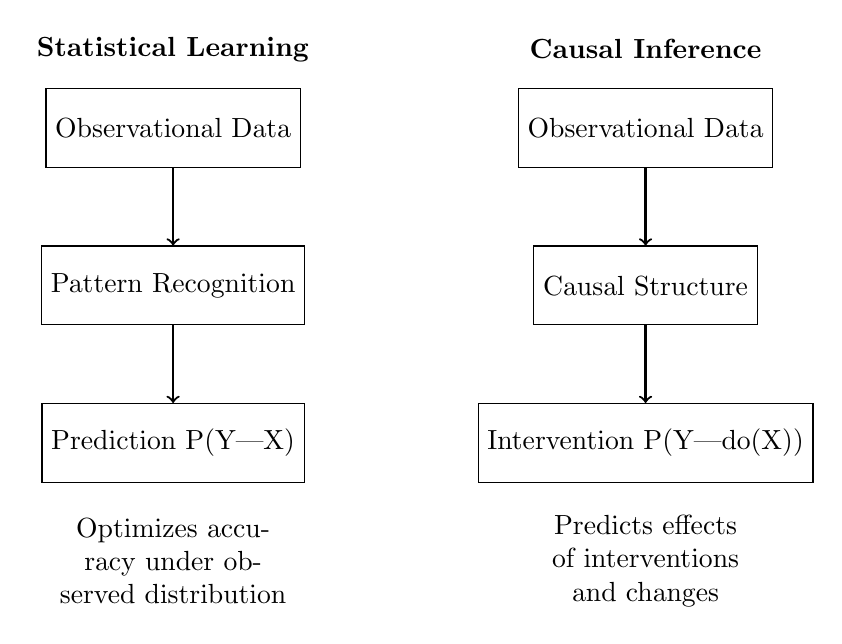
\begin{tikzpicture}[
			node distance=2cm,
			box/.style={rectangle, draw, minimum width=2.5cm, minimum height=1cm},
			arrow/.style={->, thick}
		]
		% Statistical Learning Side
		\node[box] (data1) at (0,0) {Observational Data};
		\node[box] (pattern) at (0,-2) {Pattern Recognition};
		\node[box] (predict) at (0,-4) {Prediction P(Y|X)};

		% Causal Inference Side
		\node[box] (data2) at (6,0) {Observational Data};
		\node[box] (struct) at (6,-2) {Causal Structure};
		\node[box] (inter) at (6,-4) {Intervention P(Y|do(X))};

		% Arrows for Statistical Learning
		\draw[arrow] (data1) -- (pattern);
		\draw[arrow] (pattern) -- (predict);

		% Arrows for Causal Inference
		\draw[arrow] (data2) -- (struct);
		\draw[arrow] (struct) -- (inter);

		% Labels
		\node at (0,1) {\textbf{Statistical Learning}};
		\node at (6,1) {\textbf{Causal Inference}};

		% Annotations
		\node[text width=3cm, align=center] at (0,-5.5) {Optimizes accuracy under observed distribution};
		\node[text width=3cm, align=center] at (6,-5.5) {Predicts effects of interventions and changes};

	\end{tikzpicture}
	\caption[Contrasting paradigms: Statistical learning versus causal inference]{Contrasting paradigms: Statistical learning versus causal inference. While both begin with observational data, they diverge in goals and methods.}
	\label{fig:paradigms}
\end{figure}

Figure~\ref{fig:paradigms} provides a visual representation of the fundamental differences between statistical learning and causal inference paradigms. The left side illustrates the statistical learning approach, which begins with observational data and proceeds through pattern recognition to produce predictions based on conditional distributions $P(Y|X)$. This pathway optimizes for accuracy within the observed data distribution, as indicated by the annotation below. In contrast, the right side shows the causal inference pathway, which also starts with observational data but then incorporates causal structure assumptions to enable interventional reasoning through $P(Y|\text{do}(X))$. This approach can predict the effects of interventions and changes, even when those changes fall outside the observed data distribution. The parallel structure emphasizes that while both paradigms begin with the same observational data, their divergent methodologies lead to fundamentally different capabilities and applications.

\subsubsection{When Each Paradigm Applies}

The choice between statistical learning and causal inference represents one of the most fundamental decisions in modern data science, with profound implications for methodology, interpretation, and application. This choice is not merely technical but reflects deeper philosophical commitments about the nature of scientific knowledge and the goals of analysis. Understanding when to apply each paradigm requires careful consideration of the underlying assumptions, limitations, and the specific context of the scientific question.

\paragraph{Historical Context and Philosophical Foundations:}

The distinction between these paradigms has deep roots in the philosophy of science. Statistical learning emerged from the frequentist tradition, emphasizing prediction and pattern recognition without necessarily seeking mechanistic understanding. This approach, championed by figures like Ronald Fisher and Jerzy Neyman, focuses on what can be learned from data under the assumption that the data-generating process remains stable. In contrast, causal inference builds on the structural modeling tradition, which seeks to understand the underlying mechanisms that generate observed patterns. This approach, formalized by Sewall Wright's path analysis and later developed by Judea Pearl, emphasizes the importance of causal structure in scientific reasoning.

The tension between these approaches became particularly apparent in the early 20th century with the rise of correlation analysis. While Karl Pearson championed correlation as a measure of association, Sewall Wright argued that correlation alone was insufficient for understanding causal relationships. This debate continues today in modern data science, where the availability of large datasets and sophisticated machine learning algorithms has made the distinction between correlation and causation more critical than ever.

\paragraph{Statistical Learning: Strengths and Limitations:}

Statistical learning excels in scenarios where the primary goal is prediction within a stable environment. This paradigm suffices when:

\begin{itemize}
	\item \textbf{Prediction under stable conditions}: The data-generating process remains invariant across time and space, allowing models to generalize from training to test data
	\item \textbf{Pattern recognition and anomaly detection}: Identifying unusual patterns or outliers in large datasets, such as detecting methane emission anomalies from satellite observations
	\item \textbf{Interpolation within observed ranges}: Making predictions for new observations that fall within the range of previously observed data
	\item \textbf{Real-time monitoring and forecasting}: Providing immediate predictions for operational decision-making, such as short-term methane concentration forecasts
	\item \textbf{Feature engineering and dimensionality reduction}: Discovering latent patterns in high-dimensional data, such as identifying key spectral bands in satellite imagery
\end{itemize}

However, statistical learning faces fundamental limitations when confronted with changes in the underlying system. These limitations arise from what is known as the "distributional shift problem" \cite{Quinonero-Candela2009}. When the joint distribution of variables changes; due to climate shifts, policy interventions, or expansion to new geographic regions, statistical models trained on historical data may fail catastrophically. This failure occurs because statistical learning captures correlations specific to the training distribution rather than invariant causal mechanisms.

For example, a deep learning model trained to predict methane emissions from temperature and vegetation indices might achieve excellent performance in temperate regions. However, when applied to Arctic regions where different physical processes dominate, the model may fail because the correlation structure between temperature, vegetation, and methane emissions differs fundamentally. This limitation becomes particularly problematic in environmental systems, where climate change and human interventions continuously alter the underlying dynamics.

\paragraph{Causal Inference: Necessity and Challenges:}

Causal inference becomes essential when the scientific question requires understanding mechanisms, predicting intervention effects, or generalizing across different contexts. This paradigm is necessary when:

\begin{itemize}
	\item \textbf{Evaluating interventions and policies}: Predicting the effects of specific actions, such as wetland restoration or agricultural policy changes on methane emissions
	\item \textbf{Attributing observed changes to causes}: Determining what fraction of observed methane increase is attributable to anthropogenic versus natural sources
	\item \textbf{Predicting system response to unprecedented conditions}: Understanding how methane systems will respond to climate scenarios outside historical experience
	\item \textbf{Understanding feedback mechanisms}: Identifying causal loops, such as the potential feedback between methane emissions and temperature
	\item \textbf{Generalizing across populations and contexts}: Transferring knowledge from one geographic region or time period to another
	\item \textbf{Designing robust monitoring systems}: Creating measurement strategies that remain valid under changing conditions
\end{itemize}

The mathematical foundation of causal inference lies in the distinction between observational and interventional distributions. While statistical learning models $P(Y|X)$, causal inference targets $P(Y|\text{do}(X))$, where the do-operator represents external manipulation rather than passive observation. This distinction becomes crucial when confounding variables create spurious correlations that mask true causal relationships.

Consider the relationship between wetland extent and methane emissions. Both variables may be driven by precipitation patterns, creating a spurious correlation that statistical learning would capture. Causal inference, through techniques like the adjustment formula or instrumental variables, can isolate the direct causal effect of wetland extent on emissions by accounting for the confounding influence of precipitation.

\paragraph{Integration and Complementary Roles:}

The most effective approach often involves integrating both paradigms, recognizing their complementary strengths. In comprehensive methane monitoring systems, this integration takes several forms:

\textbf{Hybrid architectures} combine statistical learning for pattern detection with causal methods for mechanistic understanding. For instance, a deep learning model might identify anomalous emission patterns in satellite data, while a causal model interprets these patterns in terms of underlying physical processes.

\textbf{Multi-stage analysis} uses statistical learning for initial data exploration and feature discovery, followed by causal inference for hypothesis testing and intervention evaluation. This approach leverages the pattern recognition capabilities of machine learning while maintaining the interpretability and generalizability of causal methods.

\textbf{Ensemble approaches} combine predictions from both paradigms, with statistical models providing baseline predictions and causal models offering mechanistic interpretations and uncertainty quantification.

For methane monitoring specifically, this integration enables both operational capabilities and scientific understanding. Statistical learning provides real-time anomaly detection and short-term forecasting from satellite data, while causal inference reveals emission mechanisms, attributes sources to specific processes, and predicts long-term responses to climate and policy changes. This dual capability is essential for transforming satellite observations from descriptive measurements into actionable environmental intelligence that can inform policy decisions and intervention strategies.

\subsection{Pearl's Causal Hierarchy}

Judea Pearl's causal hierarchy provides a formal taxonomy of causal reasoning, establishing three distinct levels of cognitive ability that cannot be reduced to one another \cite{Pearl2009}. This hierarchy, also known as the Ladder of Causation, demonstrates that different types of questions require fundamentally different types of information and inference machinery, as illustrated in Figure~\ref{fig:causal_hierarchy_pyramid}. Understanding this hierarchy is essential for recognizing what can and cannot be learned from different types of data and models.

\begin{figure}[H]
	\centering
	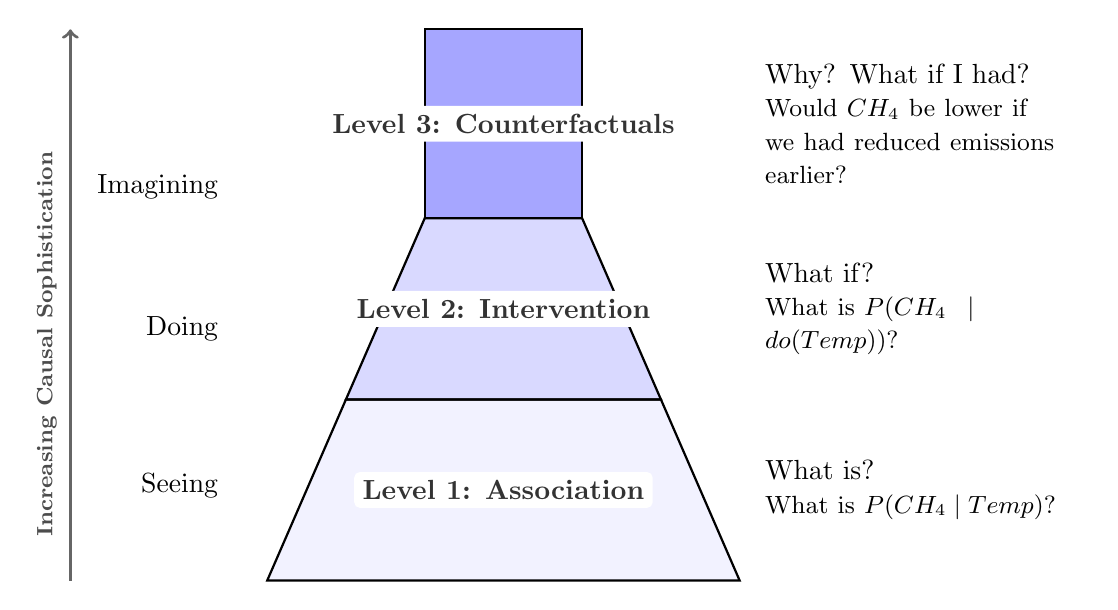
\begin{tikzpicture}
		% Define coordinates for pyramid layers (trapezoids)
		\coordinate (A1) at (0,0); \coordinate (A2) at (6,0); % Base: Level 1
		\coordinate (B1) at (1,2.3); \coordinate (B2) at (5,2.3); % Middle: Level 2
		\coordinate (C1) at (2,4.6); \coordinate (C2) at (4,4.6); % Top: Level 3

		% Draw pyramid layers (filled trapezoids)
		\fill[fill=blue!5] (A1) -- (A2) -- (B2) -- (B1) -- cycle;
		\fill[fill=blue!15] (B1) -- (B2) -- (C2) -- (C1) -- cycle;
		\fill[fill=blue!35] (C1) -- (C2) -- (4,7) -- (2,7) -- cycle;

		% Draw borders
		\draw[thick] (A1) -- (A2) -- (B2) -- (B1) -- cycle;
		\draw[thick] (B1) -- (B2) -- (C2) -- (C1) -- cycle;
		\draw[thick] (C1) -- (C2) -- (4,7) -- (2,7) -- cycle;

		% Labels for levels (inside each layer)
		\node[text=black!80, font=\bfseries, fill=white, inner sep=3pt, rounded corners=2pt] at (3,1.15) {Level 1: Association};
		\node[text=black!80, font=\bfseries, fill=white, inner sep=3pt, rounded corners=2pt] at (3,3.45) {Level 2: Intervention};
		\node[text=black!80, font=\bfseries, fill=white, inner sep=3pt, rounded corners=2pt] at (3,5.8) {Level 3: Counterfactuals};

		% Questions (right of pyramid)
		\node[right, text width=4cm, align=left] at (6.2,1.15) {What is? \\ \small What is $P(CH_4 \mid \text{Temp})$?};
		\node[right, text width=4cm, align=left] at (6.2,3.45) {What if? \\ \small What is $P(CH_4 \mid \text{do}(\text{Temp}))$?};
		\node[right, text width=4cm, align=left] at (6.2,5.8) {Why? What if I had? \\ \small Would $CH_4$ be lower if we had reduced emissions earlier?};

		% Activity labels (left of pyramid)
		\node[left, align=right] at (-0.5,1.2) {Seeing};
		\node[left, align=right] at (-0.5,3.2) {Doing};
		\node[left, align=right] at (-0.5,5.0) {Imagining};

		% Arrow showing increasing capability with improved styling
		\draw[->, very thick, black!60] (-2.5,0) -- (-2.5,7);
		% Text positioned above the arrow
		\node[text=black!70, font=\bfseries, rotate=90] at (-2.8,3) {\footnotesize Increasing Causal Sophistication};

	\end{tikzpicture}
	\caption[Pearl's Causal Hierarchy]{\small Pearl's Causal Hierarchy: A pyramid illustrating three levels of causal reasoning. Each level requires more sophisticated inference, with higher levels able to answer questions from lower levels, but not vice versa.}
	\label{fig:causal_hierarchy_pyramid}
\end{figure}

Figure~\ref{fig:causal_hierarchy_pyramid} visualizes Pearl's Causal Hierarchy through a pyramid structure that captures the three fundamental levels of causal reasoning. The pyramid's layered design emphasizes the hierarchical nature of these levels, with each higher level building upon the foundation of lower levels. The left side of the figure identifies the cognitive activities: "Seeing" for association, "Doing" for intervention, and "Imagining" for counterfactuals. The right side presents the corresponding question types and methane-specific examples that demonstrate the practical application of each level.

The hierarchy reveals a fundamental asymmetry in causal reasoning capabilities. Level 1 (Association) addresses questions about observed patterns and correlations but cannot answer interventional or counterfactual queries. Level 2 (Intervention) extends these capabilities by incorporating the do-operator, enabling reasoning about policy changes and system modifications. Level 3 (Counterfactuals) represents the most sophisticated form of causal reasoning, allowing retrospective analysis of alternative scenarios and individual-level attribution. This progression from " What is?" to "What if?" to "Why?" and "What if I had?" reflects the increasing mathematical complexity required at each level, with stronger assumptions and more sophisticated inference machinery needed for higher levels.

The transition from Level 1 to Level 2 represents the difference between prediction and action. Climate models that forecast methane concentrations under current trends operate at Level 1. Policy analysis asking how emissions would change under specific interventions requires Level 2 reasoning.

\subsubsection{Level 1: Association (Seeing)}

The first level of Pearl's causal hierarchy encompasses all questions answerable through statistical analysis of observational data. This level represents the foundation of empirical science, where we observe patterns, correlations, and conditional probabilities in the world as it naturally occurs. The mathematical framework involves joint and conditional probability distributions derived from data, forming the basis for traditional statistical inference and modern machine learning approaches.

\paragraph{Mathematical Foundation:}

Questions at this level take the form: \textquotedblleft What is the probability of Y given that I observe X?\textquotedblright Formally, this corresponds to the conditional probability:
\begin{equation}
	P(Y|X) = \frac{P(X,Y)}{P(X)}
\end{equation}

This mathematical formulation captures the statistical association between variables without making any causal claims. The conditional probability $P(Y|X)$ represents the probability of observing outcome Y when we observe X, but it does not distinguish between correlation and causation. This distinction becomes crucial when interpreting results, as correlation can arise from multiple sources: direct causation, reverse causation, confounding, or pure coincidence.

\paragraph{Historical Context and Development:}

The association level has deep roots in the development of statistical science. The concept of correlation was formalized by Francis Galton in the late 19th century and later developed by Karl Pearson into the correlation coefficient \cite{Pearl2009}. This mathematical framework enabled the systematic study of relationships between variables, laying the groundwork for modern statistical analysis. However, as noted by Sewall Wright in his development of path analysis, correlation alone cannot establish causal relationships \cite{Wright1921}.

The association level encompasses a wide range of statistical techniques, from simple correlation analysis to sophisticated machine learning algorithms. Linear regression, logistic regression, principal component analysis, and deep neural networks all operate at this level, seeking to discover patterns in observational data. These methods excel at prediction and pattern recognition but remain fundamentally limited in their ability to answer causal questions.

\paragraph{Applications in Methane Monitoring:}

In methane monitoring systems, Level 1 analysis provides essential capabilities for understanding observed patterns and making predictions. Typical Level 1 questions include:

\begin{itemize}
	\item \textbf{Pattern Recognition}: What is the correlation between temperature and methane concentrations across different regions?
	\item \textbf{Prediction}: Given current wetland extent and environmental conditions, what methane levels do we expect to observe?
	\item \textbf{Anomaly Detection}: How well can we predict emissions from observable surface properties, and what constitutes an unusual emission event?
	\item \textbf{Temporal Analysis}: What patterns exist in the seasonal cycle of atmospheric methane, and how do they vary geographically?
	\item \textbf{Feature Discovery}: Which satellite-observed variables best predict methane concentrations?
\end{itemize}

These questions are fundamental to operational methane monitoring, enabling real-time detection of emission events, seasonal forecasting, and identification of emission hotspots. Statistical models trained on historical satellite data can achieve remarkable accuracy in predicting methane concentrations from observable surface properties such as temperature, vegetation indices, and land cover characteristics.

\paragraph{Limitations and Challenges:}

Despite its utility, Level 1 analysis faces fundamental limitations that become particularly apparent in environmental systems. The primary limitation is that association captures the world as it is, not as it could be under different circumstances. All patterns are specific to the observed data distribution, and when this distribution changes—through climate shifts, policy interventions, or expansion to new geographic regions—Level 1 models may fail catastrophically.

This limitation manifests in several ways in methane monitoring:

\textbf{Distributional Shift}: Models trained on data from temperate regions may fail when applied to Arctic regions where different physical processes dominate. The correlation structure between temperature, vegetation, and methane emissions differs fundamentally across climate zones.

\textbf{Policy Interventions}: Statistical models cannot predict how methane emissions will respond to policy changes, such as wetland restoration or agricultural modifications, because these interventions create conditions outside the observed data distribution.

\textbf{Climate Change}: As the climate system evolves, historical correlations may break down, rendering prediction models obsolete.

\textbf{Confounding}: Observed correlations may reflect the influence of unmeasured confounding variables rather than direct causal relationships. For example, the correlation between rice cultivation and methane emissions may be driven by both variables responding to precipitation patterns.

\paragraph{The Machine Learning Perspective:}

Modern machine learning approaches, despite their sophistication, operate entirely at Level 1. Deep neural networks, random forests, support vector machines, and other advanced algorithms excel at discovering complex patterns in observational data but cannot reason about interventions or counterfactuals. A model trained to predict methane from satellite imagery learns the observational distribution $P(\text{CH}_4|\text{imagery})$ but cannot answer what would happen if we changed the landscape.

This limitation becomes particularly problematic when machine learning models are deployed in decision-making contexts. While these models can accurately predict methane concentrations under current conditions, they cannot provide guidance on how to reduce emissions through policy interventions. This gap between prediction and action represents one of the fundamental challenges in applying machine learning to environmental policy.

\subsubsection{Level 2: Intervention (Doing)}

The second level of Pearl's causal hierarchy addresses questions about the effects of actions and interventions, representing a fundamental shift from passive observation to active manipulation. Here we ask not what will happen given that we observe X, but what will happen if we deliberately set X to a specific value. This distinction, though subtle, is profound and represents the essence of causal reasoning.

\paragraph{The Do-Operator and Interventional Logic:}

Questions at this level involve the do-operator, introduced by Pearl to formalize the concept of intervention: \textquotedblleft What is the probability of Y if we intervene to set X to x?\textquotedblright Formally:
\begin{equation}
	P(Y|\text{do}(X=x))
\end{equation}

The do-operator represents a surgical modification of the system, where we force X to take value x while leaving all other mechanisms unchanged. This mathematical construct distinguishes interventional reasoning from observational reasoning, capturing the fundamental difference between seeing and doing. The interventional distribution $P(Y|\text{do}(X=x))$ generally differs from the observational conditional distribution $P(Y|X=x)$ due to confounding, making this distinction crucial for causal inference.

\paragraph{Historical Development and Theoretical Foundations:}

The concept of intervention has deep roots in experimental design and causal inference. Ronald Fisher's development of randomized controlled trials (RCTs) in the early 20th century provided the gold standard for establishing causal relationships \cite{Fisher1970}. The do-operator formalizes this experimental logic, allowing us to reason about interventions even when direct experimentation is impossible or unethical.

The theoretical foundation of Level 2 reasoning builds upon the work of Rubin's potential outcomes framework \cite{Rubin1974} and Pearl's structural causal models \cite{Pearl2009}. These frameworks provide different but complementary approaches to causal inference, with the do-operator serving as a unifying concept that bridges these perspectives.

\paragraph{Mathematical Distinction from Level 1:}

The key mathematical distinction between Level 1 and Level 2 lies in how they handle confounding. Consider a system where Z affects both X and Y, creating a spurious correlation between X and Y. The observational distribution conflates the direct effect of X on Y with the spurious correlation induced by Z:
\begin{equation}
	P(\mathbf{Y}|\mathbf{X}) = \sum_{\mathbf{z}} P(\mathbf{Y}|\mathbf{X},\mathbf{Z}=\mathbf{z})P(\mathbf{Z}|\mathbf{X})
\end{equation}

The interventional distribution removes this confounding by severing the link from $\mathbf{Z}$ to $\mathbf{X}$:
\begin{equation}
	P(\mathbf{Y}|\text{do}(\mathbf{X})) = \sum_{\mathbf{z}} P(\mathbf{Y}|\mathbf{X},\mathbf{Z}=\mathbf{z})P(\mathbf{Z})
\end{equation}

This adjustment formula, derived from causal assumptions encoded in a graphical model, isolates the causal effect of $\mathbf{X}$ on $\mathbf{Y}$ by removing the influence of confounding variables.

\paragraph{Applications in Methane Systems:}

In methane monitoring and policy analysis, Level 2 questions are essential for understanding the effects of potential interventions and policy changes. Typical Level 2 questions include:

\begin{itemize}
	\item \textbf{Wetland Management}: What will happen to emissions if we drain 10\% of wetlands in a specific region?
	\item \textbf{Energy Policy}: How would atmospheric methane respond to eliminating fossil fuel extraction in a particular area?
	\item \textbf{Climate Change}: What is the effect of temperature increase on methane emissions from natural sources?
	\item \textbf{Agricultural Policy}: Will changing agricultural practices, such as rice cultivation methods, reduce methane emissions?
	\item \textbf{Land Use Changes}: How would methane emissions change if we convert agricultural land to forest?
	\item \textbf{Technology Deployment}: What would be the impact of deploying methane capture technologies in specific sectors?
\end{itemize}

These questions are fundamental to policy design and environmental management, requiring causal reasoning that goes beyond pattern recognition. Answering these questions enables evidence-based policy decisions and the design of effective intervention strategies.

\paragraph{Methods for Causal Inference:}

Level 2 questions cannot be answered from observational data alone, no matter how much data we collect or how sophisticated our statistical methods. They require causal assumptions, typically encoded in structural causal models or directed acyclic graphs. With these assumptions, we can sometimes compute interventional distributions from observational data using various techniques:

\textbf{Adjustment Formula}: When all confounding variables are observed, we can use the adjustment formula to compute interventional distributions from observational data.

\textbf{Instrumental Variables}: When direct adjustment is not possible, instrumental variables can provide identification of causal effects under specific assumptions.

\textbf{Natural Experiments}: Quasi-experimental designs, such as policy changes or natural disasters, can provide identification of causal effects.

\textbf{Randomized Controlled Trials (RCT)}: When feasible, RCTs provide the most reliable estimates of causal effects, though they may not always be practical or ethical in environmental contexts.

\paragraph{Challenges in Environmental Applications:}

Environmental systems present unique challenges for Level 2 reasoning due to their complexity and interconnectedness:

\textbf{System Complexity}: Environmental systems involve numerous interacting variables, making it difficult to identify all relevant confounding factors.

\textbf{Scale and Heterogeneity}: Causal effects may vary across spatial and temporal scales, requiring careful consideration of effect heterogeneity.

\textbf{Feedback Loops}: Environmental systems often exhibit feedback mechanisms that can amplify or dampen intervention effects.

\textbf{External Validity}: Results from specific interventions may not generalize to other contexts or scales.

\textbf{Ethical and Practical Constraints}: Many environmental interventions cannot be experimentally tested due to ethical, practical, or economic constraints.

\paragraph{Integration with Level 1 Methods:}

While Level 2 reasoning requires causal assumptions beyond those needed for Level 1 analysis, it builds upon and integrates with Level 1 methods. Observational data and statistical models provide essential inputs for causal inference, with causal assumptions determining how these inputs are combined to answer interventional questions.

This integration is particularly important in methane monitoring, where we must combine satellite observations, ground-based measurements, and causal models to understand the effects of potential interventions. The combination of rich observational data with causal reasoning enables more robust and actionable insights than either approach alone.

Figure~\ref{fig:causal_hierarchy_pyramid} visualizes Pearl's Causal Hierarchy through a pyramid structure that captures the three fundamental levels of causal reasoning. The pyramid's layered design emphasizes the hierarchical nature of these levels, with each higher level building upon the foundation of lower levels. The left side of the figure identifies the cognitive activities: \textquotedblleft Seeing\textquotedblright for association, \textquotedblleft Doing\textquotedblright for intervention, and \textquotedblleft Imagining\textquotedblright for counterfactuals. The right side presents the corresponding question types and methane-specific examples that demonstrate the practical application of each level.

The hierarchy reveals a fundamental asymmetry in causal reasoning capabilities. Level 1 (Association) addresses questions about observed patterns and correlations but cannot answer interventional or counterfactual queries. Level 2 (Intervention) extends these capabilities by incorporating the do-operator, enabling reasoning about policy changes and system modifications. Level 3 (Counterfactuals) represents the most sophisticated form of causal reasoning, allowing retrospective analysis of alternative scenarios and individual-level attribution. This progression from \textquotedblleft What is?\textquotedblright to \textquotedblleft What if?\textquotedblright to \textquotedblleft Why?\textquotedblright and \textquotedblleft What if I had?\textquotedblright reflects the increasing mathematical complexity required at each level, with stronger assumptions and more sophisticated inference machinery needed for higher levels.

The transition from Level 1 to Level 2 represents the difference between prediction and action. Climate models that forecast methane concentrations under current trends operate at Level 1. Policy analysis asking how emissions would change under specific interventions requires Level 2 reasoning.

\subsubsection{Level 3: Counterfactuals (Imagining)}

The third level of Pearl's causal hierarchy encompasses counterfactual reasoning, representing the most sophisticated form of causal analysis. At this level, we ask questions about what would have happened in alternative scenarios that did not actually occur, requiring retrospective hypothetical reasoning that goes beyond both observation and intervention.

\paragraph{The Nature of Counterfactual Reasoning:}

Counterfactual reasoning represents the pinnacle of causal understanding, allowing us to reason about alternative histories and individual-level causal attribution. Questions at this level ask: \textquotedblleft Given that we observed $\mathbf{X}=x$ and $\mathbf{Y}=y$, what would $\mathbf{Y}$ have been if $\mathbf{X}$ had been $x'$?\textquotedblright Formally:
\begin{equation}
	P(\mathbf{Y}_{x'}|\mathbf{X}=x, \mathbf{Y}=y)
\end{equation}

The notation $\mathbf{Y}_{x'}$ represents the potential outcome, the value $\mathbf{Y}$ would have taken if $\mathbf{X}$ had been set to $x'$. This requires reasoning about individual cases, not just population distributions, making counterfactual analysis uniquely powerful for understanding specific events and attributing responsibility.

\paragraph{Historical and Philosophical Foundations:}

The concept of counterfactual reasoning has deep roots in philosophy, particularly in the work of David Lewis on counterfactual conditionals \cite{Lewis1973}. Lewis argued that counterfactual statements express relationships between possible worlds, where the truth of \textquotedblleft If $\mathbf{A}$ had been the case, then $\mathbf{B}$ would have been the case\textquotedblright depends on the similarity between the actual world and the closest possible world where $\mathbf{A}$ is true.

In the context of causal inference, counterfactual reasoning was formalized by Rubin's potential outcomes framework \cite{Rubin1974} and later integrated into Pearl's structural causal models \cite{Pearl2009}. This formalization enables precise mathematical treatment of counterfactual questions, making them amenable to systematic analysis.

\paragraph{Mathematical Framework and Computation:}

Counterfactual reasoning requires the strongest assumptions among the three levels, necessitating fully specified structural equations rather than just the causal graph. The computation of counterfactuals proceeds through a three-step process:

\begin{enumerate}
	\item \textbf{Abduction}: Infer the values of noise variables from observed data, essentially determining the specific state of the system that generated the observed outcome.

	\item \textbf{Action}: Modify the model to reflect the counterfactual intervention, changing the value of the variable of interest while keeping the inferred noise values constant.

	\item \textbf{Prediction}: Compute outcomes under the modified model, yielding the counterfactual outcome that would have occurred under the alternative scenario.
\end{enumerate}

This process requires complete knowledge of the structural equations governing the system, making counterfactual analysis the most demanding form of causal inference.

\paragraph{Applications in Methane Analysis:}

In methane monitoring and climate science, Level 3 questions are essential for attribution, liability assessment, and understanding the causes of specific events. Typical Level 3 questions include:

\begin{itemize}
	\item \textbf{Event Attribution}: Would the 2020 methane spike have occurred without increased wetland extent, or was it primarily driven by other factors?

	\item \textbf{Source Attribution}: What fraction of current atmospheric methane is attributable to anthropogenic sources versus natural sources?

	\item \textbf{Climate Attribution}: Would Arctic methane emissions be lower today if anthropogenic warming had been prevented?

	\item \textbf{Weather Attribution}: For a specific emission event, what would have happened under different weather conditions?

	\item \textbf{Policy Attribution}: How much of the observed methane reduction in a region is attributable to specific policy interventions versus other factors?

	\item \textbf{Individual Event Analysis}: For a particular methane leak, what would the environmental impact have been if it had been detected and repaired earlier?
\end{itemize}

These questions are fundamental to understanding the causes of observed phenomena and attributing responsibility for environmental changes.

\paragraph{The Three-Step Process in Practice:}

The three-step process for computing counterfactuals can be illustrated with a methane emission example:

\textbf{Step 1 - Abduction}: Given observed methane concentrations and environmental conditions, we infer the specific values of unobserved factors (e.g., microbial activity, soil moisture) that generated the observed outcome.

\textbf{Step 2 - Action}: We modify the model to reflect the counterfactual scenario (e.g., what if temperature had been 2\textdegree C lower), while keeping the inferred noise values constant.

\textbf{Step 3 - Prediction}: We compute the methane concentrations that would have occurred under the counterfactual conditions.

\paragraph{Challenges and Limitations:}

Counterfactual reasoning faces several significant challenges:

\textbf{Model Specification}: Counterfactual analysis requires complete specification of structural equations, which is rarely available in complex environmental systems.

\textbf{Unobserved Variables}: The abduction step requires knowledge of all relevant variables, including those that may not be directly observable.

\textbf{Non-uniqueness}: Multiple models may be consistent with the same observational data, leading to different counterfactual conclusions.

\textbf{Validation Difficulty}: Counterfactual claims cannot be directly validated through observation, making them inherently speculative.

\textbf{Computational Complexity}: Computing counterfactuals in complex systems can be computationally demanding, especially when dealing with high-dimensional data.

\paragraph{Integration with Lower Levels:}

While Level 3 reasoning requires the strongest assumptions, it builds upon and integrates with the capabilities of Levels 1 and 2. Observational data (Level 1) provides the foundation for understanding current patterns, while interventional reasoning (Level 2) helps establish causal relationships. Counterfactual reasoning (Level 3) then uses these foundations to reason about alternative scenarios.

This integration is particularly important in methane monitoring, where we must combine historical observations, experimental evidence, and counterfactual reasoning to understand the causes of observed changes and predict the effects of potential interventions.

\paragraph{Policy and Legal Implications:}

Counterfactual reasoning has profound implications for environmental policy and legal liability:

\textbf{Attribution Science}: Counterfactual analysis enables attribution of observed environmental changes to specific causes, supporting evidence-based policy decisions.

\textbf{Liability Assessment}: Counterfactual reasoning can help determine the extent to which specific actions or policies contributed to environmental outcomes.

\textbf{Policy Evaluation}: By comparing actual outcomes to counterfactual scenarios, we can assess the effectiveness of past policies and inform future decision-making.

\textbf{Climate Justice}: Counterfactual analysis can help quantify the contribution of different countries or sectors to climate change, supporting discussions of responsibility and compensation.

\subsubsection{The Hierarchy Theorem:}

The Causal Hierarchy Theorem represents one of the most fundamental results in modern causal inference, establishing the mathematical and conceptual boundaries between different types of causal reasoning. This theorem, formalized by Judea Pearl and his collaborators, demonstrates that the three levels of causal reasoning form a strict hierarchy with profound implications for the limits of what can be learned from different types of data and analytical approaches.

\paragraph{Formal Statement and Mathematical Foundation:}

The Causal Hierarchy Theorem establishes that these three levels form a strict hierarchy where higher levels can answer questions from lower levels, but not vice versa. Formally, if we can compute counterfactuals (Level 3), we can derive interventional distributions (Level 2) and observational distributions (Level 1). However, no amount of Level 1 information can answer Level 2 questions without additional causal assumptions. This asymmetry reflects the fundamental distinction between correlation and causation, a distinction that has been central to scientific reasoning since the early development of statistical methods.

The theorem's mathematical foundation lies in the relationship between different types of probability distributions. The observational distribution $P(Y|X)$ captures statistical associations but conflates causal effects with spurious correlations induced by confounding variables. The interventional distribution $P(Y|\text{do}(X))$ isolates causal effects by removing confounding through the do-operator, which represents surgical modification of the system. The counterfactual distribution $P(Y_{x'}|X=x, Y=y)$ requires the strongest assumptions, necessitating complete specification of structural equations to reason about alternative scenarios.

\paragraph{Theoretical Implications for Scientific Methodology:}

This theorem has profound implications for scientific methodology, particularly in fields where observational data dominates and experimental manipulation is limited or impossible. The theorem demonstrates that no amount of observational data alone can determine causal effects, regardless of the sophistication of statistical methods or the size of the dataset. This limitation applies equally to traditional statistical techniques and modern machine learning approaches, which operate entirely within the observational framework.

The theorem also establishes that different types of scientific questions require fundamentally different analytical approaches. Questions about patterns and correlations can be addressed through observational analysis, but questions about interventions and policy effects require causal reasoning. Questions about attribution and responsibility require the strongest form of causal reasoning, counterfactual analysis. This distinction explains why certain scientific questions remain controversial despite abundant data and sophisticated analytical techniques.

\paragraph{Implications for Environmental Monitoring and Climate Science:}

In environmental monitoring and climate science, the Causal Hierarchy Theorem explains many of the fundamental challenges facing researchers and policymakers. The attribution of observed environmental changes to specific causes, the prediction of intervention effects, and the assessment of policy effectiveness all require causal reasoning beyond what observational data alone can provide. This limitation becomes particularly apparent in methane monitoring, where satellite observations provide rich descriptive information but cannot directly answer questions about the effectiveness of emission reduction strategies.

The theorem explains why correlation-based models, however sophisticated, cannot predict intervention outcomes. A deep learning model trained on historical methane data may achieve remarkable accuracy in predicting concentrations under current conditions, but it cannot predict how emissions will respond to policy changes or technological interventions. This limitation reflects the fundamental difference between the observational distribution, which captures the world as it is, and the interventional distribution, which captures the world as it could be under different circumstances.

\paragraph{The Role of Assumptions in Causal Inference:}

The Causal Hierarchy Theorem emphasizes that moving up the hierarchy requires progressively stronger assumptions. Level 1 reasoning requires minimal assumptions beyond those needed for statistical inference. Level 2 reasoning requires causal assumptions, typically encoded in structural causal models or directed acyclic graphs. Level 3 reasoning requires the strongest assumptions, necessitating complete specification of structural equations and knowledge of all relevant variables.

These assumptions are not arbitrary but reflect our understanding of the underlying causal mechanisms. In methane systems, these assumptions might include knowledge of how temperature affects microbial activity, how precipitation influences wetland extent, or how agricultural practices impact emissions. The validity of causal conclusions depends critically on the validity of these assumptions, making transparent specification and validation of causal assumptions essential for rigorous causal inference.

\paragraph{Integration with Empirical Evidence:}

While the Causal Hierarchy Theorem establishes the theoretical limits of what can be learned from different types of data, it also provides guidance for integrating multiple sources of evidence. Observational data provides the foundation for understanding current patterns and identifying potential causal relationships. Experimental evidence, when available, can help validate causal assumptions and estimate intervention effects. Theoretical knowledge and domain expertise inform the specification of causal models and the interpretation of results.

This integration is particularly important in environmental systems, where controlled experimentation is often impossible or unethical. In such cases, researchers must rely on natural experiments, quasi-experimental designs, and careful specification of causal assumptions to draw valid causal conclusions. The theorem provides a framework for understanding the strengths and limitations of different approaches and for combining them to achieve more robust and reliable causal inference.

\begin{table}[H]
	\centering
	\caption[Examples of Questions at Each Level of Pearl's Hierarchy]{Examples of Questions at Each Level of Pearl's Hierarchy for Methane Systems}
	\label{tab:hierarchy_examples}
	\begin{tabular}{>{\raggedright\arraybackslash}p{2.2cm}|>{\raggedright\arraybackslash}p{3.8cm}|>{\raggedright\arraybackslash}p{3.8cm}|>{\raggedright\arraybackslash}p{3.8cm}}
		\hline
		\textbf{Aspect}          & \textbf{Level 1: Association}          & \textbf{Level 2: Intervention}          & \textbf{Level 3: Counterfactual}  \\
		\hline
		\textbf{Query Type}      & Probability given observation          & Probability given intervention          & Alternative histories             \\
		\textbf{Notation}        & $P(\mathbf{Y}|\mathbf{X})$             & $P(\mathbf{Y}|\text{do}(\mathbf{X}))$   & $P(\mathbf{Y}_{x'}|\mathbf{X}=x,$ \\ & & & $\mathbf{Y}=y)$ \\
		\textbf{Methane Example} & $P(\text{high CH}_4|\text{warm temp})$ & $P(\text{CH}_4|\text{do}(\text{reduce}$                                     \\ & & $\text{wetlands}))$ & What if past policies differed? \\
		\textbf{Data Needs}      & Observational                          & Experimental or causal model            & Full structural model             \\
		\textbf{Typical Methods} & Regression, ML                         & RCT, adjustment formula                 & Structural equations              \\
		\textbf{Policy Use}      & Description                            & Intervention planning                   & Attribution, liability            \\
		\hline
	\end{tabular}
\end{table}

Table~\ref{tab:hierarchy_examples} provides a systematic comparison of the three levels of Pearl's causal hierarchy, illustrating how each level addresses different types of questions in methane monitoring systems. The table demonstrates the progression from simple pattern recognition to sophisticated causal reasoning, showing how the mathematical notation, data requirements, and analytical methods become increasingly complex as we move up the hierarchy. The methane-specific examples highlight the practical relevance of each level for environmental monitoring, from basic correlation analysis to complex attribution questions that are essential for policy development and climate justice. This systematic framework helps researchers and policymakers understand which analytical approaches are appropriate for different types of questions and what additional assumptions or data are required for more sophisticated causal inference.

\paragraph{Contemporary Relevance and Future Directions:}

The Causal Hierarchy Theorem remains highly relevant in the era of big data and artificial intelligence. The increasing availability of large datasets and sophisticated machine learning algorithms has not eliminated the fundamental limitations established by the theorem. Instead, it has made these limitations more apparent and more important to address. The theorem provides a framework for understanding when and how machine learning can contribute to causal inference and when additional causal assumptions are necessary.

Future research directions include developing methods for specifying and validating causal assumptions in complex environmental systems, integrating multiple sources of evidence for more robust causal inference, and developing computational methods for counterfactual reasoning in high-dimensional systems. The theorem also provides guidance for the development of new data collection strategies, experimental designs, and analytical methods that can overcome the limitations of purely observational approaches.

The Causal Hierarchy Theorem thus serves not only as a theoretical foundation for understanding the limits of causal inference but also as a practical guide for designing research strategies and interpreting results in complex environmental systems. Its implications extend beyond methodology to inform policy decisions, risk assessment, and the allocation of research resources in environmental science and related fields.

\subsection{Structural Causal Models}

Structural Causal Models (SCMs) provide the mathematical foundation that unifies all three levels of Pearl's causal hierarchy, offering a comprehensive framework for representing, analyzing, and reasoning about causal relationships in complex systems. An SCM represents the causal mechanisms of a system through a set of structural equations that describe how each variable is determined by its direct causes and random factors. This framework enables precise formulation of causal questions and systematic derivation of their answers, making it particularly valuable for environmental systems where multiple interacting processes operate across different spatial and temporal scales.

\subsubsection{Historical Development and Theoretical Foundations}

The concept of structural equations has deep roots in econometrics and social sciences, where they were first developed to model simultaneous relationships between variables. The seminal work of Haavelmo \cite{Haavelmo1943} introduced the distinction between structural and reduced-form equations, recognizing that structural equations represent autonomous causal mechanisms that remain invariant under interventions. This insight laid the groundwork for modern causal inference, though it took several decades for the full implications to be recognized.

The formalization of SCMs as a unified framework for causal reasoning emerged primarily through the work of Judea Pearl and his collaborators in the late 1980s and 1990s \cite{Pearl2009}. Pearl's contribution was to recognize that structural equations provide a natural language for encoding causal assumptions and that these assumptions, when combined with probability theory, enable systematic computation of interventional and counterfactual distributions. This synthesis of structural modeling with probabilistic reasoning created a powerful framework that could handle the complexity of real-world systems while maintaining mathematical rigor.

The development of SCMs was motivated by the recognition that traditional statistical methods, while powerful for pattern recognition and prediction, were fundamentally limited in their ability to answer causal questions. Correlation analysis, regression modeling, and even sophisticated machine learning approaches could identify associations and make predictions, but they could not distinguish between correlation and causation or predict the effects of interventions. SCMs address this limitation by explicitly representing causal mechanisms through structural equations, enabling reasoning about what would happen under different circumstances.

\subsubsection{Mathematical Framework and Components}

A Structural Causal Model $\mathcal{M}$ consists of four fundamental components that together specify the complete causal structure of a system:

\begin{equation}
	\mathcal{M} = \langle \mathbf{U}, \mathbf{V}, \mathbf{F}, P(\mathbf{U}) \rangle
\end{equation}

\textbf{Exogenous Variables} $\mathbf{U} = \{U_1, ..., U_n\}$ represent factors determined outside the model, including random disturbances, measurement errors, unmodeled influences, and external interventions. These variables are not explained by the model but influence the endogenous variables through the structural equations. In environmental systems, exogenous variables might include random weather fluctuations, measurement noise in satellite sensors, unobserved microbial population dynamics, or policy interventions. The key assumption is that these exogenous variables are independent of each other, representing the modularity of different causal mechanisms.

\textbf{Endogenous Variables} $\mathbf{V} = \{V_1, ..., V_m\}$ are the variables of interest, determined within the model by structural equations. These represent the observable quantities that we seek to understand and predict. For methane monitoring systems, endogenous variables include atmospheric methane concentrations, emission rates, temperature, precipitation, wetland extent, vegetation indices, and anthropogenic activities. These variables are typically observable, at least in principle, though they may be subject to measurement error or sampling limitations.

\textbf{Structural Equations} $\mathbf{F} = \{f_1, ..., f_m\}$ specify how each endogenous variable is determined by its direct causes:

\begin{equation}
	V_i = f_i(\text{PA}_i, U_i)
\end{equation}

where $\text{PA}_i \subseteq \mathbf{V} \setminus \{V_i\}$ represents the direct causes (parents) of $V_i$ in the causal graph. These equations encode our understanding of causal mechanisms and need not be linear or even have closed-form expressions. They simply assert that $V_i$ is some function of its parents and noise, representing the autonomous mechanism that determines $V_i$'s value.

\textbf{Probability Distribution} $P(\mathbf{U})$ specifies the joint distribution of exogenous variables, typically assumed to have independent components for simplicity. This distribution captures the stochastic nature of the system and determines the observational distribution over endogenous variables.

\subsubsection{The Modularity Principle and Invariance}

A fundamental property of SCMs is the modularity principle, also known as autonomy or invariance. This principle states that each structural equation represents an autonomous mechanism that remains invariant when other mechanisms are modified. This invariance underlies the computation of interventions and distinguishes causal relationships from mere statistical associations.

The modularity principle has profound implications for environmental systems. Consider a methane emission system where temperature affects both wetland extent and microbial activity. The structural equation for methane emissions might be:

\begin{equation}
	\text{CH}_4 = f_M(\text{Wetlands}, \text{Temperature}, \text{Agriculture}, U_M)
\end{equation}

The modularity principle asserts that this equation remains valid even if we intervene to change wetland extent through drainage or restoration. The mechanism by which temperature affects methane emissions (through microbial activity) remains unchanged, even though the overall methane levels may change due to the wetland intervention.

This invariance property enables counterfactual reasoning: we can ask what methane levels would have been under different wetland conditions while keeping all other mechanisms constant. This capability is essential for policy analysis, where we need to predict the effects of specific interventions without changing the underlying physical and biological processes.

\subsubsection{From Structural Equations to Causal Graphs}

Every SCM induces a directed acyclic graph (DAG) that provides a visual representation of the causal structure. In this graph:

\begin{itemize}
	\item Nodes represent variables (both endogenous and sometimes exogenous)
	\item Directed edges connect parents to children according to structural equations
	\item The absence of an edge indicates no direct causal effect
\end{itemize}

The causal graph serves multiple purposes: it makes causal assumptions transparent, enables visual reasoning about complex relationships, and provides the mathematical machinery for causal inference through concepts like d-separation and the backdoor criterion.

For methane monitoring systems, the causal graph might include nodes for temperature, precipitation, wetland extent, agricultural activity, and methane concentrations, with edges representing direct causal influences. This graphical representation helps researchers communicate their assumptions, identify potential confounding variables, and design appropriate analysis strategies.

\subsubsection{Computing Interventions: The Do-Calculus}

The do-operator formally represents interventions in SCMs, enabling computation of interventional distributions $P(Y|\text{do}(X=x))$. Computing these distributions involves three steps:

\begin{enumerate}
	\item \textbf{Modify the SCM}: Replace the structural equation for X with the constant assignment X = x
	\item \textbf{Compute the induced distribution}: Propagate the intervention through the remaining equations
	\item \textbf{Marginalize}: Sum over exogenous variables to obtain the interventional distribution
\end{enumerate}

For the methane example, computing the effect of wetland restoration involves:

\begin{align}
	P(\text{CH}_4|\text{do}(\text{Wetlands}=w)) & = \sum_{t,p,a} P(\text{CH}_4|w,a,t) \\
	                                            & \quad \times P(a)P(t)P(p|t)
\end{align}

Note that under intervention, the dependence of wetlands on precipitation disappears—we force wetlands to value w regardless of precipitation. This is the key distinction between observational and interventional distributions.

\subsubsection{Counterfactual Reasoning and the Three-Step Process}

SCMs enable counterfactual reasoning through their structural equations, allowing us to answer questions about alternative scenarios that did not actually occur. The computation of counterfactuals proceeds through a three-step process:

\begin{enumerate}
	\item \textbf{Abduction}: Given observed data, infer the values of exogenous variables U that generated the observed outcome
	\item \textbf{Action}: Modify the model to reflect the counterfactual scenario (e.g., what if wetlands had been 20\% smaller?)
	\item \textbf{Prediction}: Compute outcomes under the modified model with the inferred U values
\end{enumerate}

This process requires fully specified structural equations, not just the causal graph. Different functional forms can yield different counterfactual predictions even with the same graph structure, highlighting the importance of accurate model specification.

For methane systems, counterfactual reasoning enables attribution questions such as: "What would methane levels have been if anthropogenic emissions had been eliminated?" or "How much of the observed methane increase is attributable to climate change versus human activities?" These questions are essential for policy evaluation and climate justice considerations.

\subsubsection{Extensions and Limitations}

While SCMs provide a powerful framework for causal reasoning, they come with important limitations that must be acknowledged in environmental applications:

\textbf{Causal Sufficiency}: Standard SCMs assume no unmeasured confounders—all common causes of measured variables are included in the model. This assumption rarely holds in environmental systems where many processes remain unobserved or unmeasurable. Extensions like structural equation models with latent variables and partial ancestral graphs address this limitation but require additional assumptions.

\textbf{Acyclicity}: SCMs require directed acyclic graphs, yet many environmental systems exhibit feedback loops. Temperature affects methane emissions, which affect radiative forcing, which affects temperature. Extensions to cyclic models exist but complicate inference and require specialized methods.

\textbf{Functional Form Specification}: While the causal graph may be identifiable from data, the specific functional forms of structural equations typically are not. Different functions consistent with the same graph can yield different quantitative predictions, requiring careful consideration of domain knowledge and sensitivity analysis.

\textbf{Stationarity}: SCMs typically assume time-invariant relationships, yet environmental systems exhibit regime shifts, tipping points, and evolving dynamics. Climate change itself represents non-stationarity in Earth system relationships, requiring time-varying or regime-dependent models.

\textbf{Scale and Aggregation}: Environmental processes operate across multiple spatial and temporal scales, creating challenges for model specification and interpretation. Aggregating fine-scale processes into coarse-scale variables can introduce aggregation bias and mask important causal relationships.

Despite these challenges, SCMs remain the most comprehensive framework for causal reasoning, providing the mathematical foundation for moving from correlation to causation in environmental monitoring. The key is to acknowledge these limitations explicitly and design analysis strategies that are robust to violations of model assumptions.

\subsubsection{Integration with Environmental Monitoring}

For satellite-based methane monitoring, SCMs provide a natural framework for integrating multiple data sources and addressing the complex interactions between atmospheric, terrestrial, and anthropogenic processes. The structural equations can incorporate satellite observations, ground-based measurements, and auxiliary data while maintaining the causal interpretation necessary for policy applications.

The modularity principle is particularly valuable for environmental systems, where interventions (such as wetland restoration or emission reduction policies) target specific mechanisms while leaving others unchanged. This property enables prediction of intervention effects even when the specific intervention has not been observed in historical data.

Moreover, the graphical representation of SCMs facilitates communication between scientists, policymakers, and stakeholders. Causal graphs make assumptions transparent and enable discussion of alternative models, supporting evidence-based decision-making in environmental policy.

In summary, Structural Causal Models provide the mathematical foundation for rigorous causal analysis in environmental monitoring, enabling the transition from descriptive pattern recognition to mechanistic understanding of Earth system processes. While they require careful attention to assumptions and limitations, they offer the most comprehensive framework for addressing the causal questions that are essential for effective environmental policy and climate action.

\subsubsection{Formal Definition and Components}

A Structural Causal Model $\mathcal{M}$ consists of four components:
\begin{equation}
	\mathcal{M} = \langle \mathbf{U}, \mathbf{V}, \mathbf{F}, P(\mathbf{U}) \rangle
\end{equation}

Each component plays a specific role in capturing the causal structure:

\textbf{Exogenous Variables} $\mathbf{U} = \{U_1, ..., U_n\}$: These represent factors determined outside the model, random disturbances, measurement errors, or unmodeled influences. In methane systems, exogenous variables might include random weather fluctuations, measurement noise in satellite sensors, or unobserved microbial population dynamics. We typically cannot observe these directly but must account for their effects.

\textbf{Endogenous Variables} $\mathbf{V} = \{V_1, ..., V_m\}$: These are the variables of interest, determined within the model by structural equations. For methane monitoring, endogenous variables include atmospheric concentrations, emission rates, temperature, wetland extent, and anthropogenic activities. These are typically observable, at least in principle.

\textbf{Structural Equations} $\mathbf{F} = \{f_1, ..., f_m\}$: Each equation specifies how an endogenous variable is determined by its direct causes:
\begin{equation}
	V_i = f_i(\text{PA}_i, U_i)
\end{equation}

where $\text{PA}_i \subseteq \mathbf{V} \setminus \{V_i\}$ represents the direct causes (parents) of $V_i$. These equations encode our understanding of causal mechanisms. They need not be linear or even have closed-form expressions, they simply assert that $V_i$ is some function of its parents and noise.

\textbf{Probability Distribution} $P(\mathbf{U})$: This specifies the joint distribution of exogenous variables, typically assumed to have independent components for simplicity.

\subsubsection{Example: Simplified Methane System}

Consider a simplified model of methane dynamics:
\begin{align}
	\text{Temperature}   & = f_T(\text{Solar}, U_T)                                            \\
	\text{Precipitation} & = f_P(\text{Temperature}, U_P)                                      \\
	\text{Wetlands}      & = f_W(\text{Precipitation}, \text{Temperature}, U_W)                \\
	\text{Agriculture}   & = f_A(\text{Economic}, U_A)                                         \\
	\text{CH}_4          & = f_M(\text{Wetlands}, \text{Agriculture}, \text{Temperature}, U_M)
\end{align}

This SCM encodes our causal assumptions: temperature affects precipitation and wetlands; both wetlands and agriculture directly influence methane emissions; temperature has both direct effects on methane (through microbial activity) and indirect effects (through wetlands).

The structural equations might take specific functional forms based on domain knowledge:
\begin{align}
	\text{CH}_4 & = \alpha \cdot \text{Wetlands} \cdot \exp(\beta \cdot \text{Temperature}) \\
	            & \quad + \gamma \cdot \text{Agriculture} + U_M
\end{align}

This assumes multiplicative effects of temperature on wetland emissions (representing temperature-dependent microbial activity) and additive contributions from agriculture.

\subsubsection{From SCMs to Causal Graphs}

Every SCM induces a directed acyclic graph (DAG) where:
\begin{itemize}
	\item Nodes represent variables (both endogenous and sometimes exogenous)
	\item Directed edges connect parents to children according to structural equations
	\item The absence of an edge indicates no direct causal effect
\end{itemize}

\begin{figure}[h!]
	\centering
	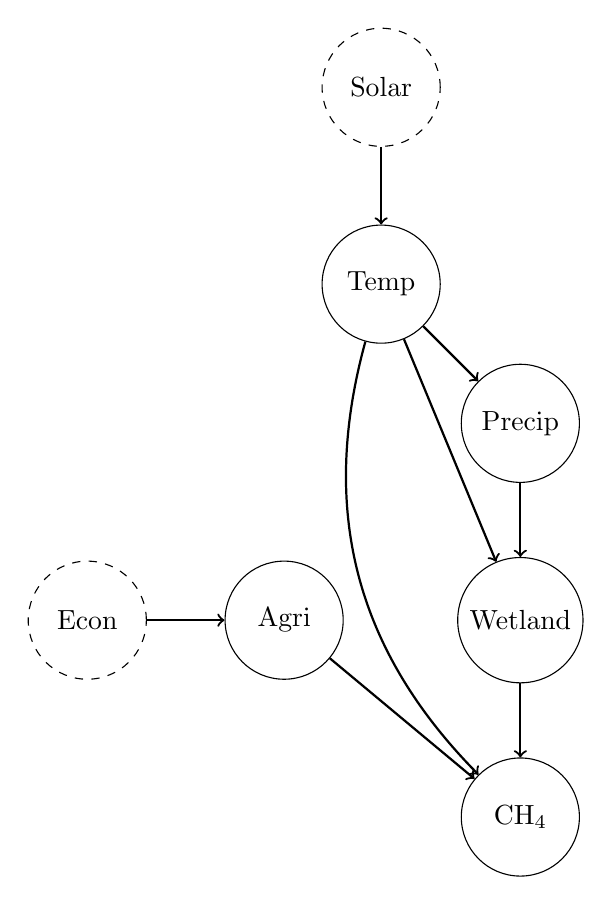
\begin{tikzpicture}[
			node distance=2.5cm,
			var/.style={circle, draw, minimum width=1.5cm},
			latent/.style={circle, draw, dashed, minimum width=1.5cm},
			arrow/.style={->, thick}
		]
		% Nodes
		\node[var] (temp) {Temp};
		\node[var] (precip) [below right of=temp] {Precip};
		\node[var] (wet) [below of=precip] {Wetland};
		\node[var] (agri) [left of=wet, node distance=3cm] {Agri};
		\node[var] (ch4) [below of=wet] {CH$_4$};
		\node[latent] (solar) [above of=temp] {Solar};
		\node[latent] (econ) [left of=agri] {Econ};

		% Edges
		\draw[arrow] (solar) -- (temp);
		\draw[arrow] (temp) -- (precip);
		\draw[arrow] (temp) -- (wet);
		\draw[arrow] (precip) -- (wet);
		\draw[arrow] (wet) -- (ch4);
		\draw[arrow] (agri) -- (ch4);
		\draw[arrow] (temp) to[bend right=30] (ch4);
		\draw[arrow] (econ) -- (agri);

	\end{tikzpicture}
	\caption[Causal graph induced by the simplified methane SCM]{Causal graph induced by the simplified methane SCM. Solid circles represent endogenous (observed) variables, dashed circles represent exogenous factors. Edges encode direct causal relationships from structural equations.}
	\label{fig:methane_dag}
\end{figure}

The graph in Figure~\ref{fig:methane_dag} provides visual intuition about causal relationships while maintaining mathematical precision. Path-based reasoning on the graph corresponds to algebraic manipulation of structural equations, enabling researchers to trace causal pathways from exogenous drivers through intermediate variables to the target methane concentrations. This graphical representation facilitates communication of causal assumptions between scientists, policymakers, and stakeholders, while providing the mathematical machinery for systematic causal inference through concepts like d-separation and the backdoor criterion.

\subsubsection{The Modularity Principle}

A fundamental property of SCMs is modularity: each structural equation represents an autonomous mechanism that remains invariant when other mechanisms are modified. This principle, also known as autonomy or invariance, underlies the computation of interventions and distinguishes causal relationships from mere statistical associations. The modularity principle has profound implications for environmental systems, where interventions such as wetland restoration or emission reduction policies target specific mechanisms while leaving others unchanged. When we intervene to set $V_i = v$, we replace the structural equation for $V_i$ with the constant assignment $V_i = v$, keep all other structural equations unchanged, and compute the resulting distribution. This "surgery" on the model corresponds to removing incoming edges to $V_i$ in the causal graph, and the modularity principle asserts that intervening on one mechanism does not alter others. For example, draining wetlands changes methane emissions but does not change how temperature affects precipitation, enabling prediction of intervention effects even when the specific intervention has not been observed in historical data.

\subsubsection{Computing Interventions}

The do-operator formally represents interventions in SCMs, enabling computation of interventional distributions $P(Y|\text{do}(X=x))$ that capture the effects of external manipulations rather than passive observations. Computing these distributions involves three systematic steps: first, we modify the SCM by replacing the structural equation for X with the constant assignment X = x; second, we compute the induced distribution by propagating the intervention through the remaining equations; and third, we marginalize by summing over exogenous variables to obtain the interventional distribution. For the methane example, computing the effect of wetland restoration involves the calculation $P(\text{CH}_4|\text{do}(\text{Wetlands}=w)) = \sum_{t,p,a} P(\text{CH}_4|w,a,t) \times P(a)P(t)P(p|t)$, where we note that precipitation's dependence on wetlands disappears under intervention since we force wetlands to value w regardless of precipitation. This key distinction between observational and interventional distributions enables prediction of policy effects and intervention outcomes that cannot be determined from correlation analysis alone.

\subsubsection{Counterfactual Reasoning}

SCMs enable counterfactual reasoning through their structural equations, allowing us to answer questions about alternative scenarios that did not actually occur, such as "What would methane levels have been if wetlands had been 20\% smaller?" The computation of counterfactuals proceeds through a systematic three-step process: first, we perform abduction by inferring the values of exogenous variables U from observed data; second, we take action by modifying the model to reflect the counterfactual scenario (e.g., reducing wetlands by 20\%); and third, we make predictions by computing outcomes under the modified model with the inferred U values. This process requires fully specified structural equations, not just the causal graph, and different functional forms can yield different counterfactual predictions even with the same graph structure, highlighting the importance of accurate model specification for reliable counterfactual inference.

\subsubsection{Limitations and Challenges}

While SCMs provide a powerful framework for causal reasoning, they come with important limitations that must be acknowledged in environmental applications. The assumption of causal sufficiency, which requires that all common causes of measured variables are included in the model, rarely holds in environmental systems where many processes remain unobserved or unmeasurable, such as subsurface microbial dynamics or complex atmospheric chemistry. The requirement for acyclicity in directed acyclic graphs presents another challenge, as many environmental systems exhibit feedback loops where temperature affects methane emissions, which in turn affect radiative forcing and ultimately temperature again, though extensions to cyclic models exist but complicate inference significantly. Functional form specification represents a further limitation, as while the causal graph may be identifiable from data, the specific functional forms of structural equations typically are not, and different functions consistent with the same graph can yield different quantitative predictions requiring careful consideration of domain knowledge and sensitivity analysis. Additionally, the assumption of stationarity, which requires time-invariant relationships, conflicts with the reality that environmental systems exhibit regime shifts, tipping points, and evolving dynamics, with climate change itself representing non-stationarity in Earth system relationships. Despite these challenges, SCMs remain the most comprehensive framework for causal reasoning, providing the mathematical foundation for moving from correlation to causation in environmental monitoring, with the key being to acknowledge these limitations explicitly and design analysis strategies that are robust to violations of model assumptions.

\subsection{Graphical Causal Representations}

Building upon the mathematical foundation of Structural Causal Models, graphical representations provide the visual and computational framework that transforms abstract structural equations into intuitive, analyzable causal structures. While SCMs define the formal mathematical relationships through structural equations, causal graphs offer a complementary perspective that makes these relationships explicit, testable, and communicable. The transition from structural equations to graphical representations is natural and essential: every SCM induces a directed acyclic graph where nodes represent variables and edges encode the direct causal influences specified in the structural equations. This graphical approach serves multiple purposes: it makes causal assumptions transparent, enables visual reasoning about complex relationships, and provides the mathematical machinery for causal inference through concepts like d-separation and the backdoor criterion. Different types of graphs capture different aspects of causal structure, from complete specifications to equivalence classes representing our uncertainty about the true causal relationships. The graphical approach to causal modeling emerged from the recognition that complex causal systems require intuitive yet mathematically rigorous representations that can be communicated between researchers, validated against domain knowledge, and systematically analyzed for inference. This graphical framework provides a unified language for expressing causal assumptions, testing their implications, and deriving predictions that can be validated against observational data, thereby bridging the gap between theoretical causal models and practical applications in environmental monitoring.

\subsubsection{Directed Acyclic Graphs (DAGs): The Foundation}

A Directed Acyclic Graph consists of nodes representing variables connected by directed edges indicating direct causal relationships. The "acyclic" constraint ensures no variable can be its own cause, even indirectly. In a DAG $G = (\mathbf{V}, \mathbf{E})$, an edge $\mathbf{V}_i \rightarrow \mathbf{V}_j$ asserts that $\mathbf{V}_i$ has a direct causal effect on $\mathbf{V}_j$, an effect that persists even when controlling for all other variables in the graph.

DAGs encode independence relationships through the d-separation criterion. This graphical criterion determines which variables are conditionally independent given others, providing a complete characterization of the independence constraints implied by the causal structure. Understanding d-separation requires recognizing three basic patterns:

\textbf{Chains} ($\mathbf{A} \rightarrow \mathbf{B} \rightarrow \mathbf{C}$): Information flows from $\mathbf{A}$ to $\mathbf{C}$ through $\mathbf{B}$. If we condition on $\mathbf{B}$ (observe its value), we block this flow, making $\mathbf{A}$ and $\mathbf{C}$ independent given $\mathbf{B}$. In methane systems, temperature might affect wetland extent, which affects emissions. Knowing wetland extent blocks the indirect path from temperature to emissions.

\textbf{Forks} ($\mathbf{A} \leftarrow \mathbf{B} \rightarrow \mathbf{C}$): A common cause $\mathbf{B}$ creates correlation between $\mathbf{A}$ and $\mathbf{C}$. Conditioning on $\mathbf{B}$ blocks this spurious correlation. Seasonal cycles might drive both temperature and vegetation patterns. Controlling for season removes their spurious correlation.

\textbf{Colliders} ($\mathbf{A} \rightarrow \mathbf{B} \leftarrow \mathbf{C}$): Two causes converge on a common effect. Initially, $\mathbf{A}$ and $\mathbf{C}$ are independent. However, conditioning on $\mathbf{B}$ (or its descendants) creates correlation between $\mathbf{A}$ and $\mathbf{C}$. If both wetlands and agriculture affect methane levels, then observing unusually high methane makes wetland and agricultural sources negatively correlated, if one is high, the other must be lower to explain the observation. Figure~\ref{fig:dag_patterns} illustrates these three fundamental patterns and their behavior under conditioning.

\begin{figure}[h!]
	\centering
	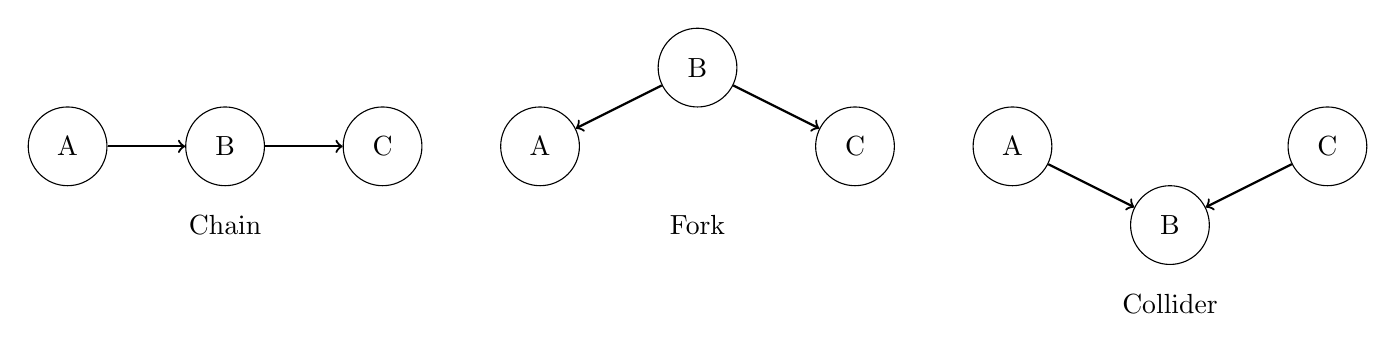
\begin{tikzpicture}[
			node distance=2cm,
			var/.style={circle, draw, minimum width=1cm},
			arrow/.style={->, thick}
		]
		% Chain
		\node[var] (a1) at (0,0) {A};
		\node
		[var] (b1) at (2,0) {B};
		\node[var] (c1) at (4,0) {C};
		\draw[arrow] (a1) -- (b1);
		\draw[arrow] (b1) -- (c1);
		\node at (2,-1) {Chain};

		% Fork
		\node[var] (a2) at (6,0) {A};
		\node[var] (b2) at (8,1) {B};
		\node[var] (c2) at (10,0) {C};
		\draw[arrow] (b2) -- (a2);
		\draw[arrow] (b2) -- (c2);
		\node at (8,-1) {Fork};

		% Collider
		\node[var] (a3) at (12,0) {A};
		\node[var] (b3) at (14,-1) {B};
		\node[var] (c3) at (16,0) {C};
		\draw[arrow] (a3) -- (b3);
		\draw[arrow] (c3) -- (b3);
		\node at (14,-2) {Collider};

	\end{tikzpicture}
	\caption[Three fundamental patterns in DAGs]{Three fundamental patterns in DAGs. Chains and forks transmit correlation that conditioning blocks. Colliders block correlation until conditioning induces it.}
	\label{fig:dag_patterns}
\end{figure}

The d-separation criterion formalizes these intuitions: A path between $\mathbf{X}$ and $\mathbf{Y}$ is blocked by conditioning set $\mathbf{Z}$ if it contains either (i) a chain or fork with the middle node in $\mathbf{Z}$, or (ii) a collider with neither the collider nor its descendants in $\mathbf{Z}$. Variables $\mathbf{X}$ and $\mathbf{Y}$ are d-separated by $\mathbf{Z}$ if all paths between them are blocked.

The power of d-separation lies in its completeness: it characterizes all conditional independence relationships implied by the causal structure. The Markov property connects graph structure to probability:
\begin{equation}
	\mathbf{X} \perp_d \mathbf{Y} | \mathbf{Z} \text{ in } G \implies \mathbf{X} \perp \mathbf{Y} | \mathbf{Z} \text{ in } P
\end{equation}

This means d-separation in the graph implies conditional independence in any distribution compatible with the causal structure. The faithfulness assumption, which states that the only conditional independencies in the distribution are those implied by d-separation in the graph, provides the converse relationship, enabling inference of causal structure from observed independencies. Together, these properties establish a bidirectional relationship between graph structure and probability distributions that forms the foundation for causal discovery algorithms and provides the theoretical justification for inferring causal relationships from observational data.

\subsubsection{Completed Partially Directed Acyclic Graphs (CPDAGs): Representing Equivalence}

While a true causal DAG uniquely determines independence relationships, the reverse is not true, multiple DAGs can encode the same conditional independencies. These Markov equivalent DAGs form equivalence classes, represented by CPDAGs.

A CPDAG contains:
\begin{itemize}
	\item \textbf{Directed edges}: Present with the same orientation in all equivalent DAGs
	\item \textbf{Undirected edges}: Oriented differently across equivalent DAGs
\end{itemize}

Two DAGs are Markov equivalent if and only if they have:
\begin{enumerate}
	\item The same skeleton (underlying undirected graph)
	\item The same v-structures (colliders)
\end{enumerate}

This characterization, known as the Verma-Pearl theorem, provides a complete criterion for Markov equivalence. It reveals what can and cannot be learned from observational data alone under the faithfulness assumption.

Consider three variables: Temperature (T), Wetlands (W), and Methane (M). The following DAGs are Markov equivalent:
\begin{itemize}
	\item T → W → M
	\item T ← W → M
	\item T ← W ← M
\end{itemize}

All share the same skeleton (T-W-M) and have no v-structures. Their CPDAG would show T, W, M with all edges undirected, indicating that observational data cannot determine causal direction without additional assumptions.

However, $\mathbf{T} \rightarrow \mathbf{W} \leftarrow \mathbf{M}$ is not equivalent to the others, it contains a v-structure at $\mathbf{W}$. If data shows $\mathbf{T}$ and $\mathbf{M}$ are marginally independent but become dependent when conditioning on $\mathbf{W}$, this uniquely identifies the v-structure. Figure~\ref{fig:cpdag_example} demonstrates this concept by showing three Markov equivalent DAGs and their resulting CPDAG representation.

\begin{figure}[H]
	\centering
	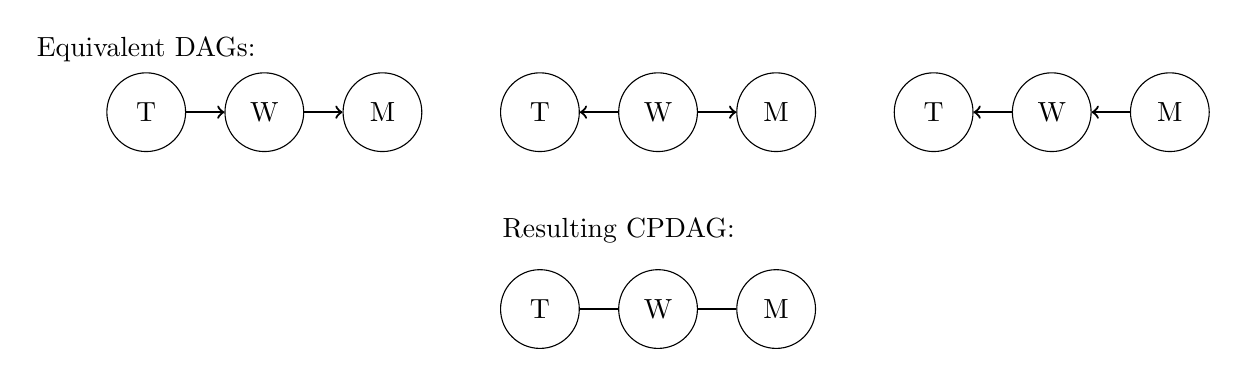
\begin{tikzpicture}[
			node distance=2cm,
			var/.style={circle, draw, minimum width=1cm},
			arrow/.style={->, thick},
			line/.style={-, thick}
		]
		% Equivalent DAGs
		\node at (0,0.8) {Equivalent DAGs:};

		% DAG 1
		\node[var] (t1) at (0,0) {T};
		\node[var] (w1) at (1.5,0) {W};
		\node[var] (m1) at (3,0) {M};
		\draw[arrow] (t1) -- (w1);
		\draw[arrow] (w1) -- (m1);

		% DAG 2
		\node[var] (t2) at (5,0) {T};
		\node[var] (w2) at (6.5,0) {W};
		\node[var] (m2) at (8,0) {M};
		\draw[arrow] (w2) -- (t2);
		\draw[arrow] (w2) -- (m2);

		% DAG 3
		\node[var] (t3) at (10,0) {T};
		\node[var] (w3) at (11.5,0) {W};
		\node[var] (m3) at (13,0) {M};
		\draw[arrow] (w3) -- (t3);
		\draw[arrow] (m3) -- (w3);

		% CPDAG
		\node at (6,-1.5) {Resulting CPDAG:};
		\node[var] (t4) at (5,-2.5) {T};
		\node[var] (w4) at (6.5,-2.5) {W};
		\node[var] (m4) at (8,-2.5) {M};
		\draw[line] (t4) -- (w4);
		\draw[line] (w4) -- (m4);

	\end{tikzpicture}
	\caption[Three Markov equivalent DAGs and their CPDAG representation]{Three Markov equivalent DAGs and their CPDAG representation. Undirected edges in the CPDAG indicate orientational uncertainty that cannot be resolved from observational data alone.}
	\label{fig:cpdag_example}
\end{figure}

CPDAGs reveal a fundamental limitation: observational data, no matter how abundant, cannot fully determine causal structure. Additional assumptions (like causal ordering from temporal precedence) or interventional data are needed to orient undirected edges. This limitation reflects the inherent ambiguity in causal inference from observational data alone, where multiple causal structures can generate identical statistical patterns. The CPDAG representation provides a principled way to express this uncertainty, distinguishing between relationships that can be determined from observational data and those that require additional information or assumptions. This framework is particularly valuable in environmental applications where controlled experiments are often impossible and researchers must rely on natural experiments, temporal precedence, or domain knowledge to resolve causal ambiguities.

\subsubsection{Maximal Ancestral Graphs (MAGs) and Partial Ancestral Graphs (PAGs): Handling Hidden Variables}

Real-world systems invariably include unmeasured variables, subsurface processes affecting methane emissions, unobserved economic factors driving land use, or complex microbial dynamics. MAGs and PAGs extend the graphical framework to represent causal relationships in the presence of latent confounders.

A MAG uses three types of edges:
\begin{itemize}
	\item \textbf{Directed} ($\rightarrow$): Direct causation
	\item \textbf{Bidirected} ($\leftrightarrow$): Confounding by unmeasured common cause
	\item \textbf{Undirected} (, ): Selection bias from conditioning
\end{itemize}

The bidirected edge is particularly important for environmental systems. If $\mathbf{X} \leftrightarrow \mathbf{Y}$, some unmeasured variable affects both. For instance, soil moisture might be unmeasured but affect both vegetation indices and methane emissions, inducing a bidirected edge between them in the MAG.

PAGs extend this further by representing equivalence classes of MAGs, analogous to how CPDAGs represent equivalence classes of DAGs. PAG edges use additional symbols:

\begin{itemize}
	\item Circle ($\circ$): Endpoint is arrow in some MAGs, tail in others
	\item Arrow ($\rightarrow$): Endpoint is arrow in all MAGs
	\item Tail ($-$): Endpoint is tail in all MAGs
\end{itemize}

Edge interpretations in PAGs:
\begin{itemize}
	\item $X \rightarrow Y$: X causes Y (possibly through unmeasured mediators)
	\item $X \leftrightarrow Y$: X and Y share unmeasured common cause(s)
	\item $X \circ\!\rightarrow Y$: Either causal or confounded
	\item $X \circ\!-\!\circ Y$: Any relationship possible
\end{itemize}

The circle endpoints in PAGs represent the uncertainty introduced by unmeasured variables, providing a conservative representation that acknowledges the limitations of observational data while still enabling meaningful causal inference. This conservative approach is particularly important in environmental applications where many relevant variables cannot be directly measured, such as subsurface microbial processes, atmospheric chemistry, or human decision-making factors that influence land use and emissions. Table~\ref{tab:graph_types} provides a comprehensive comparison of these different graphical representations, highlighting their respective purposes, edge types, and use cases for causal inference in environmental monitoring.

\begin{table}[H]
	\centering
	\caption[Comparison of Graphical Representations]{Comparison of Graphical Representations}
	\label{tab:graph_types}
	\begin{tabular}{>{\raggedright\arraybackslash}p{2cm}|>{\raggedright\arraybackslash}p{3cm}|>{\raggedright\arraybackslash}p{3cm}|>{\raggedright\arraybackslash}p{3cm}|>{\raggedright\arraybackslash}p{3cm}}
		\hline
		\textbf{Property}  & \textbf{DAG}                  & \textbf{CPDAG}            & \textbf{MAG}                       & \textbf{PAG}                     \\
		\hline
		Purpose            & Single causal model           & Equivalence class of DAGs & Single model with hidden variables & Equivalence class of MAGs        \\
		Edge Types         & Directed only                 & Directed + Undirected     & Directed + Bidirected + Undirected & Additional circle endpoints      \\
		Hidden Variables   & Not represented               & Not represented           & Implicit in bidirected edges       & Implicit with uncertainty        \\
		What it represents & Complete causal specification & Observational equivalence & Marginal causal structure          & Marginal equivalence             \\
		Use Case           & Known structure               & Structure learning result & Known hidden confounding           & Learning with hidden confounding \\
		\hline
	\end{tabular}
\end{table}

\subsubsection{Practical Implications for Methane Monitoring}

The choice of graphical representation depends on available knowledge and assumptions:

\textbf{Use DAGs when}:
\begin{itemize}
	\item Causal relationships are well-established from domain knowledge
	\item All relevant variables are measured
	\item The goal is to compute specific causal effects
	\item Temporal ordering provides clear causal direction
\end{itemize}

\textbf{Use CPDAGs when}:
\begin{itemize}
	\item Learning causal structure from observational data
	\item Some causal directions remain uncertain
	\item Multiple models are equally consistent with data
	\item Identifying what experiments would resolve ambiguity
\end{itemize}

\textbf{Use PAGs when}:
\begin{itemize}
	\item Important variables are unmeasurable (soil microbes, economic factors)
	\item Confounding is suspected but sources unknown
	\item Conservative inference is needed
	\item Satellite data provides incomplete system observation
\end{itemize}

For satellite-based methane monitoring, PAGs often provide the most realistic representation. We cannot measure all relevant processes, microbial populations, subsurface conditions, human decision-making, yet these latent factors certainly influence observed relationships. PAGs acknowledge this uncertainty while still enabling meaningful causal inference. The conservative nature of PAGs makes them particularly suitable for policy applications where overconfidence in causal relationships could lead to ineffective or counterproductive interventions. By explicitly representing uncertainty about causal relationships, PAGs provide a framework for designing robust monitoring strategies that can adapt to new information and for communicating the limitations of causal conclusions to stakeholders and policymakers. This approach aligns with the precautionary principle in environmental policy, where acknowledging uncertainty is essential for responsible decision-making in the face of complex, incompletely understood systems.

\subsection{Causal Discovery for Non-Temporal Data}

Having established the theoretical foundations of Structural Causal Models and their graphical representations, we now turn to the practical challenge of inferring causal structure from observational data. Causal discovery represents the inverse problem to causal modeling: rather than specifying causal assumptions and deriving their implications, we seek to identify causal relationships from patterns in data. This approach reverses the traditional statistical workflow where models are specified a priori, instead systematically exploring the space of possible causal structures to identify relationships consistent with observed data. The graphical representations introduced in the previous section (DAGs, CPDAGs, MAGs, and PAGs) provide the mathematical framework within which these discovery algorithms operate, enabling the systematic identification of causal relationships from observational data alone. This data-driven approach proves particularly valuable in complex environmental systems where complete prior knowledge is unavailable and controlled experiments are infeasible, such as methane monitoring where we must infer emission sources and their drivers from satellite observations. The development of causal discovery methods emerged from the recognition that traditional statistical approaches, while powerful for pattern recognition and prediction, were fundamentally limited in their ability to distinguish correlation from causation. Early work in this field was motivated by the need to understand complex systems where controlled experimentation was impossible or unethical, leading to the development of systematic approaches for inferring causal structure from observational data alone.

The fundamental challenge lies in the underdetermination problem: multiple causal structures can generate identical observational distributions, as illustrated by the Markov equivalence classes discussed in the context of CPDAGs. This fundamental limitation reflects the inherent ambiguity in causal inference from observational data alone, where the same statistical patterns can arise from different underlying causal mechanisms. Causal discovery methods address this through different strategies, each making distinct assumptions about the data-generating process and leveraging different aspects of the graphical framework. These assumptions range from the faithfulness assumption, which states that the only conditional independencies in the data are those implied by the causal structure, to more specific assumptions about functional forms and noise distributions. Understanding these assumptions and their implications is crucial for appropriate method selection and interpretation, particularly in environmental applications where the validity of these assumptions may vary across different spatial and temporal scales. The choice of discovery method depends not only on the available data but also on the specific research questions, the nature of the underlying system, and the level of uncertainty that can be tolerated in the results. The following sections examine the three main approaches to causal discovery: constraint-based methods that learn from conditional independence relationships, score-based methods that optimize over graph space, and functional causal models that exploit distributional asymmetries to identify causal direction.

\subsubsection{Constraint-Based Methods: Learning from Independence}

Constraint-based algorithms reconstruct causal structure by systematically testing conditional independence relationships in data, building directly on the d-separation properties of causal graphs introduced in the previous section. The core insight is that causal structure constrains which variables can be independent given others, and these constraints, in turn, reveal the underlying causal graph. This approach leverages the fundamental connection between causal structure and conditional independence that forms the basis of the graphical causal framework, making it particularly well-suited for applications where the underlying causal mechanisms are complex and not well understood. In environmental systems like methane monitoring, where multiple interacting processes operate across different scales, constraint-based methods can identify causal relationships without requiring detailed knowledge of the underlying physical or biological mechanisms.

\textbf{The PC Algorithm: Foundation of Constraint-Based Discovery}

The PC algorithm, named after its creators Peter Spirtes and Clark Glymour, exemplifies the constraint-based approach. It operates in two distinct phases:

\textbf{Phase 1: Skeleton Discovery}. Starting with a complete undirected graph, the algorithm progressively removes edges based on conditional independence tests. For each pair of variables $(X_i, X_j)$, it searches for a conditioning set $\mathbf{S}$ that renders them independent. Algorithm~\ref{alg:pc-skeleton} presents the skeleton discovery phase of the PC algorithm, which systematically tests conditional independence relationships to identify the underlying graph structure.

\begin{algorithm}[h!]
	\caption[PC Algorithm for Skeleton Discovery]{PC Algorithm for Skeleton Discovery}
	\label{alg:pc-skeleton}
	\Input{A complete undirected graph}
	\Output{A skeleton graph with separation sets}
	\BlankLine
	Initialize with a complete undirected graph\;
	\For{$\ell = 0$ to $\max(\textnormal{degree})$}
	{
		\For{each adjacent pair $(X_i, X_j)$}
		{
			\For{each subset $\mathbf{S} \subseteq \textnormal{Adj}(X_i) \setminus \{X_j\}$ with $|\mathbf{S}| = \ell$}
			{
				\lIf{$\mathbf{X}_i \perp \mathbf{X}_j \mid \mathbf{S}$}
				{
					Remove edge $X_i - X_j$\;
					Store $\mathbf{S}$ as separation set $\mathbf{S}_{ij}$\;
					\textbf{break}\;
				}
			}
		}
	}
\end{algorithm}

The algorithm exploits efficiency by testing conditioning sets of increasing size, stopping when independence is detected. This staged approach dramatically reduces computational complexity compared to testing all possible conditioning sets, making it feasible to analyze high-dimensional datasets that are common in environmental monitoring applications. The progressive nature of the algorithm also provides a natural stopping criterion and helps identify the minimal conditioning sets that render variables independent, which can be valuable for understanding the underlying causal mechanisms.

\textbf{Phase 2: Orientation}. With the skeleton established, the algorithm orients edges to create a DAG. The fundamental rule identifies v-structures:

If the skeleton contains $X_i - X_k - X_j$ with $X_i$ and $X_j$ non-adjacent, and $X_k \notin \mathbf{S}_{ij}$, then orient as $X_i \rightarrow X_k \leftarrow X_j$.

The logic is compelling: if $X_k$ were not a collider, it would d-separate $X_i$ and $X_j$, so it should appear in their separation set. Its absence indicates a v-structure. This v-structure identification is crucial for resolving causal direction in observational data, as it represents one of the few cases where causal direction can be uniquely determined from conditional independence relationships alone. In environmental applications, identifying v-structures can help distinguish between direct causal relationships and spurious correlations induced by common causes.

Meek's orientation rules complete the process, propagating orientations while maintaining acyclicity. Figure~\ref{fig:meek_rules} illustrates two key orientation rules that prevent the creation of new v-structures and cycles during the orientation process.

\begin{figure}[H]
	\centering
	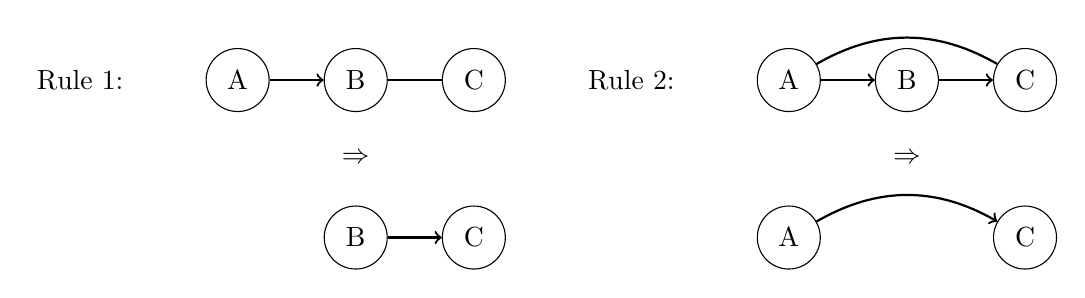
\begin{tikzpicture}[
			node distance=1.5cm,
			var/.style={circle, draw, minimum width=0.8cm},
			arrow/.style={->, thick},
			line/.style={-, thick}
		]
		% Meek Rule 1
		\node at (0,0) {Rule 1:};
		\node[var] (a1) at (2,0) {A};
		\node[var] (b1) at (3.5,0) {B};
		\node[var] (c1) at (5,0) {C};
		\draw[arrow] (a1) -- (b1);
		\draw[line] (b1) -- (c1);
		\node at (3.5,-1) {$\Rightarrow$};
		\node[var] (b1b) at (3.5,-2) {B};
		\node[var] (c1b) at (5,-2) {C};
		\draw[arrow] (b1b) -- (c1b);

		% Meek Rule 2
		\node at (7,0) {Rule 2:};
		\node[var] (a2) at (9,0) {A};
		\node[var] (b2) at (10.5,0) {B};
		\node[var] (c2) at (12,0) {C};
		\draw[arrow] (a2) -- (b2);
		\draw[arrow] (b2) -- (c2);
		\draw[line] (a2) to[bend left=30] (c2);
		\node at (10.5,-1) {$\Rightarrow$};
		\node[var] (a2b) at (9,-2) {A};
		\node[var] (c2b) at (12,-2) {C};
		\draw[arrow] (a2b) to[bend left=30] (c2b);

	\end{tikzpicture}
	\caption[Meek's orientation rules]{Meek's orientation rules. Rule 1 prevents new v-structures; Rule 2 prevents cycles. Additional rules handle more complex patterns.}
	\label{fig:meek_rules}
\end{figure}

\textbf{Statistical Testing Considerations}

The choice of conditional independence test represents one of the most critical decisions in constraint-based causal discovery, as it fundamentally determines the algorithm's ability to distinguish genuine causal relationships from spurious associations. This choice involves navigating a complex trade-off between statistical power, computational efficiency, and robustness to violations of underlying assumptions. The theoretical foundations of these tests derive from different branches of statistical theory, each offering distinct advantages and limitations that must be carefully considered in the context of environmental monitoring applications.

\paragraph{Test Selection and Theoretical Foundations:}

The selection of an appropriate conditional independence test requires understanding both the mathematical foundations and practical implications of each approach:

\begin{itemize}
	\item \textbf{Partial correlation tests} (Gaussian assumption): These tests evaluate whether the partial correlation coefficient $\rho_{\mathbf{X}\mathbf{Y}|\mathbf{Z}}$ equals zero, implementing the null hypothesis $H_0: \rho_{\mathbf{X}\mathbf{Y}|\mathbf{Z}} = 0$ against the alternative $H_1: \rho_{\mathbf{X}\mathbf{Y}|\mathbf{Z}} \neq 0$. The test statistic follows a t-distribution under the null hypothesis, with degrees of freedom adjusted for the conditioning set size. While computationally efficient and theoretically well-understood, these tests rely critically on the assumption of multivariate normality, which may be violated in environmental systems characterized by heavy-tailed distributions, seasonal patterns, or threshold-driven processes.

	\item \textbf{Mutual information tests} (nonparametric): These tests evaluate the null hypothesis $H_0: I(\mathbf{X};\mathbf{Y}|\mathbf{Z}) = 0$, where $I(\mathbf{X};\mathbf{Y}|\mathbf{Z})$ represents the conditional mutual information between variables $\mathbf{X}$ and $\mathbf{Y}$ given conditioning set $\mathbf{Z}$. Unlike partial correlation tests, mutual information tests make no distributional assumptions and can detect both linear and nonlinear dependencies. However, they require estimation of probability densities, which becomes increasingly challenging in high-dimensional spaces and can lead to reduced statistical power compared to parametric alternatives.

	\item \textbf{Kernel-based tests} (nonlinear): These tests leverage reproducing kernel Hilbert spaces (RKHS) to detect complex, potentially nonlinear dependencies without explicitly specifying functional forms. The Hilbert-Schmidt Independence Criterion (HSIC) and its conditional variants provide a framework for testing independence in high-dimensional spaces. While offering superior flexibility for capturing complex relationships, kernel-based tests introduce additional computational complexity and require careful selection of kernel functions and hyperparameters.
\end{itemize}

\paragraph{Multiple Testing and False Discovery Control:}

The multiple testing problem represents one of the most significant challenges in constraint-based causal discovery, particularly in high-dimensional environmental applications. With $p$ variables, the PC algorithm performs $O(p^2)$ pairwise independence tests in the initial phase, followed by $O(p^3)$ conditional independence tests in subsequent phases. This exponential growth in the number of tests creates a severe multiple testing problem that can lead to inflated false discovery rates and spurious causal relationships.

Modern approaches to addressing this challenge include:

\begin{itemize}
	\item \textbf{False Discovery Rate (FDR) control}: Methods such as the Benjamini-Hochberg procedure control the expected proportion of false discoveries among all rejected null hypotheses. This approach provides a principled framework for balancing statistical power against false positive control, though it requires careful consideration of the dependency structure among tests.

	\item \textbf{Stability selection}: This approach evaluates the stability of discovered relationships across bootstrap samples or random subsamples of the data. Relationships that appear consistently across multiple samples are considered more reliable, providing a data-driven approach to reducing false discoveries.

	\item \textbf{Adaptive significance levels}: These methods adjust significance levels based on the local structure of the graph, recognizing that tests in sparse regions of the graph may require different thresholds than tests in dense regions.
\end{itemize}

\paragraph{Environmental-Specific Considerations:}

The multiple testing problem is particularly acute in environmental applications due to several unique characteristics of environmental datasets:

\begin{itemize}
	\item \textbf{High dimensionality}: Environmental monitoring datasets often include hundreds of variables representing different environmental factors (temperature, precipitation, vegetation indices), land use types, atmospheric constituents, and temporal lags. This high dimensionality exponentially increases the number of required tests.

	\item \textbf{Strong autocorrelation}: Environmental time series exhibit strong temporal dependencies that can create spurious relationships and complicate independence testing. Traditional independence tests may fail to account for these temporal dependencies, leading to inflated false positive rates.

	\item \textbf{Seasonal and periodic patterns}: Environmental systems exhibit strong seasonal and periodic patterns that can create apparent relationships between variables that are actually driven by shared temporal structure rather than genuine causal mechanisms.

	\item \textbf{Measurement uncertainty}: Environmental measurements often include substantial uncertainty due to sensor limitations, atmospheric conditions, and processing algorithms. This measurement uncertainty can propagate through independence tests, affecting their reliability.
\end{itemize}

\paragraph{Impact on Causal Discovery:}

The choice of significance level and multiple testing correction method can significantly impact the resulting causal structure, with profound implications for the interpretation and application of discovered relationships. Conservative approaches that prioritize false positive control may miss genuine causal relationships, particularly in complex environmental systems where causal effects may be subtle or context-dependent. Conversely, liberal approaches that prioritize statistical power may identify spurious relationships that do not reflect genuine causal mechanisms.

This trade-off between sensitivity and specificity must be carefully considered in the context of the specific research question and the potential consequences of false positive versus false negative discoveries. In policy-relevant applications, false positives may lead to misguided interventions or resource allocation, while false negatives may result in missed opportunities for effective environmental management. The development of robust, context-aware approaches to multiple testing correction represents an active area of research in causal discovery, with particular relevance for environmental applications where the stakes of incorrect inference are high.

\textbf{The FCI Algorithm: Handling Latent Confounders}

The Fast Causal Inference (FCI) algorithm extends PC to scenarios with unmeasured confounders. It produces PAGs rather than DAGs, acknowledging uncertainty from hidden variables.

FCI's key innovation is conditioning on possible ancestors rather than just adjacent nodes. This broader conditioning set can d-separate variables even when confounders create spurious adjacencies in the observed graph. The algorithm adds orientation rules specific to ancestral graphs, distinguishing between direct causation and confounding. This approach is particularly valuable in environmental systems where many relevant variables are unmeasured, such as subsurface processes, atmospheric chemistry, or human decision-making factors. By conditioning on a broader set of variables, FCI can identify spurious relationships that arise from unmeasured confounders and provide more reliable causal conclusions in the presence of latent variables.

For methane systems where microbial processes, subsurface conditions, and human decisions remain unmeasured, FCI provides more reliable inference than PC, though at increased computational cost. The ability to handle latent confounders makes FCI particularly valuable in environmental applications where many relevant variables cannot be directly observed, such as subsurface microbial populations, atmospheric chemistry processes, or human decision-making factors that influence land use and emissions. By explicitly acknowledging the presence of unmeasured variables, FCI produces more conservative and realistic causal conclusions that better reflect the uncertainty inherent in observational environmental data.

\subsubsection{Score-Based Methods: Optimization Over Graph Space}

Score-based methods formulate causal discovery as an optimization problem: find the graph that optimally explains the observed data according to some scoring criterion. This approach transforms the combinatorial problem of graph search into a more tractable optimization framework, providing an alternative to constraint-based methods that can be more efficient for high-dimensional datasets. Unlike constraint-based methods that rely on statistical testing of conditional independencies, score-based approaches evaluate entire graph structures and can incorporate prior knowledge about the system through the scoring function. This makes them particularly useful in applications where domain expertise can guide the search process or where the data-generating process is well-understood but the specific causal relationships are unknown.

\textbf{Scoring Functions: Balancing Fit and Complexity}

The Bayesian Information Criterion (BIC) exemplifies score-based approaches:
\begin{equation}
	\text{BIC}(G) = \log P(\mathbf{D}|\hat{\theta}_G, G) - \frac{k_G \log n}{2}
\end{equation}

The first term measures how well graph $G$ with maximum likelihood parameters $\hat{\theta}_G$ fits data $\mathbf{D}$. The second term penalizes complexity, where $k_G$ counts free parameters and $n$ is sample size.

For Gaussian distributions with linear relationships:
\begin{equation}
	\text{BIC}(G) = -\frac{n}{2} \log|\hat{\Sigma}| - \frac{k_G \log n}{2}
\end{equation}

where $\hat{\Sigma}$ is the empirical covariance matrix and $k_G = |E| + p$ for $|E|$ edges and $p$ variables.

Alternative scoring functions include:
\begin{itemize}
	\item \textbf{AIC}: Uses penalty $2k_G$ (less aggressive than BIC)
	\item \textbf{BGe score}: Bayesian score with Gaussian likelihood and Wishart prior
	\item \textbf{BDeu score}: Bayesian Dirichlet score for discrete variables
\end{itemize}

\textbf{Greedy Equivalence Search (GES): Efficient Optimization}

Exhaustive search over all possible DAGs is computationally intractable, the number of DAGs grows super-exponentially with variables. GES navigates this space efficiently through greedy local search, providing a practical solution to the combinatorial explosion problem that makes exhaustive search impossible even for moderate numbers of variables. This efficiency makes GES particularly suitable for environmental applications where datasets may contain dozens or hundreds of variables representing different environmental factors, land use types, atmospheric constituents, and temporal patterns.

GES operates in two phases:

\textbf{Forward phase}: Starting from an empty graph, repeatedly add the edge that maximally increases the score, continuing until no improvement is possible.

\textbf{Backward phase}: Remove edges that increase the score (noting that removing edges can increase penalized scores by reducing complexity).

The algorithm's power comes from score decomposability:
\begin{equation}
	\mathcal{S}(G) = \sum_{i=1}^{p} \mathcal{S}_i(\mathbf{X}_i, \text{PA}_i^G)
\end{equation}

This allows local computation of score changes without re-evaluating the entire graph. Adding edge $X_j \rightarrow X_i$ only affects the local score for $X_i$. This local computation property is crucial for the efficiency of GES, as it enables the algorithm to evaluate potential graph modifications without recomputing scores for the entire graph structure. This property is particularly valuable in environmental applications where the causal structure may be sparse and local modifications are more common than global restructuring.

GES provides theoretical guarantees: under faithfulness and correct model specification, it consistently recovers the true CPDAG as sample size increases. Recent variants like Fast GES (FGES) incorporate parallelization and caching for improved scalability, making them suitable for large-scale environmental datasets. The theoretical consistency of GES makes it particularly valuable for applications where the underlying causal structure is expected to be sparse and where computational efficiency is important, such as analyzing high-dimensional satellite data or large-scale environmental monitoring networks.

\subsubsection{Functional Causal Models: Exploiting Asymmetry}

Functional causal model approaches leverage asymmetries in the joint distribution to identify causal direction, representing a fundamentally different approach from constraint-based and score-based methods. While correlation is symmetric, causation often introduces detectable asymmetries in how variables relate, providing a basis for identifying causal direction from observational data alone. This approach is particularly powerful because it can resolve the ambiguity inherent in Markov equivalence classes by exploiting distributional properties that go beyond conditional independence relationships. In environmental applications, where causal direction is often critical for understanding system dynamics and designing interventions, functional causal models can provide unique insights that other methods cannot.

\textbf{Linear Non-Gaussian Acyclic Model (LiNGAM): Identifiability through Non-Gaussianity}

LiNGAM achieves what seems impossible: unique identification of the causal DAG from observational data, without equivalence classes. The key insight is that non-Gaussianity breaks the symmetry that makes linear Gaussian models unidentifiable.

The model assumes:
\begin{equation}
	\mathbf{X} = \mathbf{B}\mathbf{X} + \boldsymbol{\varepsilon}
\end{equation}

where $\mathbf{B}$ is strictly lower-triangular (encoding causal ordering) and $\boldsymbol{\varepsilon}$ contains independent non-Gaussian noise.

Rewriting: $\mathbf{X} = (\mathbf{I} - \mathbf{B})^{-1}\boldsymbol{\varepsilon} = \mathbf{A}\boldsymbol{\varepsilon}$

Independent Component Analysis (ICA) can recover $\mathbf{A}$ (up to permutation and scaling) from observed $\mathbf{X}$. The permutation that makes $\mathbf{W} = \mathbf{A}^{-1}$ lower-triangular reveals the causal ordering.

The algorithm proceeds:
\begin{enumerate}
	\item Apply ICA to recover mixing matrix $\mathbf{A}$
	\item Find permutation making $\mathbf{W} = \mathbf{A}^{-1}$ maximally lower-triangular
	\item Set $\mathbf{B} = \mathbf{I} - \mathbf{W}$ to obtain causal structure
\end{enumerate}

For methane systems, LiNGAM could uniquely identify whether temperature drives emissions or emissions affect local temperature (through radiative effects), provided relationships are approximately linear and noise is non-Gaussian, often satisfied with log-transformed environmental variables. This unique identification capability makes LiNGAM particularly valuable for resolving causal direction in environmental systems where the direction of influence is critical for understanding feedback mechanisms and designing effective interventions. The requirement for non-Gaussian noise is often naturally satisfied in environmental data due to the complex, nonlinear processes that generate them, making LiNGAM a practical tool for environmental causal inference.

\textbf{Additive Noise Models (ANM): Nonlinear Identification}

ANMs extend the identifiability principle to nonlinear relationships:
\begin{equation}
	\mathbf{Y} = f(\mathbf{X}) + \mathbf{N}_Y, \quad \mathbf{N}_Y \perp \mathbf{X}
\end{equation}

The key insight: in the correct causal direction, the residual noise is independent of the input. In the wrong direction, the backward model $X = g(Y) + N_X$ will generally have $N_X$ dependent on $Y$.

The identification principle relies on the genericity argument: for most nonlinear functions $f$ and noise distributions, the independence holds only in the true causal direction. Exceptions exist (e.g., linear Gaussian case) but are measure-zero in the space of possible models. This genericity argument provides theoretical justification for the identifiability of causal direction in most practical scenarios, making ANMs particularly valuable for environmental applications where relationships are often nonlinear and noise distributions are typically non-Gaussian due to the complex, interacting processes that generate environmental data.

The algorithm tests both directions:
\begin{enumerate}
	\item Regress $\mathbf{Y}$ on $\mathbf{X}$: $\hat{f} = \arg\min_{f \in \mathcal{F}} \mathbb{E}[(\mathbf{Y} - f(\mathbf{X}))^2]$
	\item Test independence: $\mathbf{N}_Y = \mathbf{Y} - \hat{f}(\mathbf{X})$ independent of $\mathbf{X}$?
	\item Repeat with $\mathbf{X}$ on $\mathbf{Y}$
	\item Select direction with stronger independence
\end{enumerate}

Regression uses nonparametric methods (kernel regression, Gaussian processes) to avoid functional form assumptions. Independence testing employs kernel-based tests (HSIC) or information-theoretic measures.

\textbf{Post-Nonlinear Models (PNL): Additional Flexibility}

PNL models add further flexibility:
\begin{equation}
	\mathbf{Y} = g(f(\mathbf{X}) + \mathbf{N}_X) + \mathbf{N}_Y
\end{equation}

This captures scenarios where measurement processes introduce additional nonlinearity. While more flexible, PNL models are harder to identify and require stronger assumptions or larger sample sizes. This additional flexibility makes PNL models particularly relevant for environmental applications where measurement processes, such as satellite retrievals or ground-based sensors, may introduce nonlinear transformations that affect the observed relationships between variables. However, the increased complexity of PNL models means they require more data and stronger assumptions for reliable identification, making them most suitable for applications where the measurement process is well-understood and sufficient data is available.

\subsubsection{Practical Considerations for Method Selection}

Choosing appropriate causal discovery methods requires understanding their assumptions, strengths, and limitations. Table~\ref{tab:discovery_methods} provides a comprehensive comparison of the different causal discovery approaches discussed in this section, highlighting their key assumptions, strengths, and limitations for methane monitoring applications.

\begin{table}[H]
	\centering
	\caption[Comparison of Causal Discovery Approaches for Methane Monitoring]{Comparison of Causal Discovery Approaches for Methane Monitoring}
	\label{tab:discovery_methods}
	\begin{tabular}{>{\raggedright\arraybackslash}p{2.5cm}|>{\raggedright\arraybackslash}p{3.5cm}|>{\raggedright\arraybackslash}p{3.5cm}|>{\raggedright\arraybackslash}p{3.5cm}}
		\hline
		\textbf{Method} & \textbf{Key Assumptions}          & \textbf{Strengths}                            & \textbf{Limitations}                      \\
		\hline
		PC/FCI          & Faithfulness, causal Markov       & Nonparametric, handles latent variables (FCI) & Multiple testing, sensitive to violations \\
		GES/FGES        & Correct model specification       & Theoretically consistent, efficient search    & Parametric assumptions, local optima      \\
		LiNGAM          & Linear, non-Gaussian, acyclic     & Unique identification                         & Linearity restriction                     \\
		ANM             & Additive noise, generic functions & Handles nonlinearity                          & Pairwise only, additivity assumption      \\
		\hline
	\end{tabular}
\end{table}

For satellite-based methane monitoring, the choice of causal discovery method depends on the specific characteristics of the dataset and research question. The literature suggests several considerations for method selection:

\begin{enumerate}
	\item \textbf{Presence of unmeasured confounders}: When unmeasured variables are suspected (e.g., subsurface processes, atmospheric chemistry), FCI provides a principled approach to handle latent confounding by producing PAGs that acknowledge uncertainty from hidden variables \cite{Runge2019_2}.

	\item \textbf{Nonlinear relationships}: When environmental processes suggest nonlinear dependencies (e.g., temperature-methane relationships in wetlands), ANM methods can provide additional constraints for edge orientation beyond what constraint-based methods alone can achieve \cite{Peters2014}.

	\item \textbf{Validation requirements}: The integration of domain knowledge and temporal constraints can help resolve ambiguities that remain after statistical testing, particularly when multiple causal structures are consistent with the observed data.

	\item \textbf{Robustness assessment}: Testing consistency across different methods and data subsamples provides a practical approach to assessing the reliability of discovered relationships, though the theoretical foundations for such validation remain an active area of research.
\end{enumerate}

The convergence of evidence across multiple methods with different assumptions strengthens confidence in discovered relationships. Discrepancies highlight where assumptions may be violated or data insufficient, guiding further investigation. This multi-method approach is particularly important in environmental applications where the validity of individual method assumptions may vary across different spatial and temporal scales or environmental conditions. By combining methods with different strengths and limitations, researchers can develop more robust and reliable causal conclusions that are less sensitive to violations of specific assumptions. This approach also provides a framework for communicating uncertainty to stakeholders and policymakers, acknowledging the limitations of observational causal inference while still providing actionable insights for environmental management and policy development.

\subsection{Causal Discovery for Temporal Data}
\label{subsec:temporal_causal}

The transition from static to temporal causal discovery represents a fundamental paradigm shift in causal inference, particularly critical for environmental monitoring systems where processes evolve dynamically over time. Building upon the structural causal models and graphical representations established in previous sections, temporal causal discovery introduces the dimension of time as both a constraint and an opportunity. In the context of methane monitoring through satellite observations, where atmospheric concentrations, emission sources, and environmental drivers exhibit complex temporal dependencies across multiple time scales, understanding causal relationships requires specialized methods that exploit temporal structure while accounting for its inherent complexities.

The temporal setting fundamentally alters the causal discovery landscape. Unlike static scenarios where causal direction must be inferred from distributional asymmetries or intervention data, temporal precedence provides natural directional constraints: causes precede their effects. This temporal ordering significantly reduces the space of possible causal structures, offering a powerful constraint that can resolve ambiguities present in static causal discovery. However, this apparent advantage comes with substantial challenges. Autocorrelation in time series can create spurious relationships that mimic causal effects, different environmental processes operate at distinct time scales (daily weather patterns versus seasonal cycles versus long-term climate trends), and feedback loops between variables violate the acyclicity assumption central to many static causal discovery methods. Furthermore, the presence of hidden confounders that vary over time, measurement errors that propagate over time, and the need to handle missing data in satellite observations all complicate temporal causal inference.

For methane monitoring specifically, these challenges manifest themselves in several critical ways. Methane emissions from natural sources (wetlands, permafrost) and anthropogenic activities (agriculture, fossil fuel extraction) exhibit distinct temporal signatures. Wetland emissions follow seasonal cycles driven by temperature and precipitation, with peak emissions typically occurring during warm, wet periods \cite{Pandey2017}. Permafrost thaw releases methane episodically during warming events, creating irregular temporal patterns that differ from steady anthropogenic sources \cite{Knox2024}. Agricultural emissions show seasonal patterns (rice cultivation) and event-driven spikes (manure management). Satellite observations of atmospheric methane concentrations integrate these diverse sources, creating a complex temporal signal that requires sophisticated causal discovery methods to unravel. In addition, atmospheric transport processes, meteorological conditions, and sensor characteristics all introduce temporal dependencies that must be considered in causal analysis.

The methodological landscape for temporal causal discovery has evolved significantly over the past decades, from early predictive frameworks like Granger causality to modern multivariate methods that handle high-dimensional, autocorrelated time series. This evolution reflects both theoretical advances in understanding temporal causality and practical demands from applications in climate science, neuroscience, and economics. For methane monitoring, the availability of high-frequency satellite data from instruments such as TROPOMI, combined with auxiliary environmental datasets (temperature, precipitation, vegetation indices, land use), creates opportunities for sophisticated temporal causal analysis that can inform both scientific understanding and policy decisions.

The temporal setting offers both opportunities and complications. Unlike static data, where causal direction must be inferred from distributional asymmetries, temporal precedence provides clear directional information. However, autocorrelation can create spurious relationships, different processes operate at different time scales, and feedback loops violate the acyclicity assumption central to many methods. Successfully navigating these challenges requires specialized approaches that exploit the temporal structure while accounting for its complexities. Figure~\ref{fig:temporal_causal_structures} illustrates the key differences between static and temporal causal structures, highlighting how temporal precedence constrains possible causal relationships while introducing new challenges such as autocorrelation and feedback loops.

\begin{figure}[H]
	\centering
	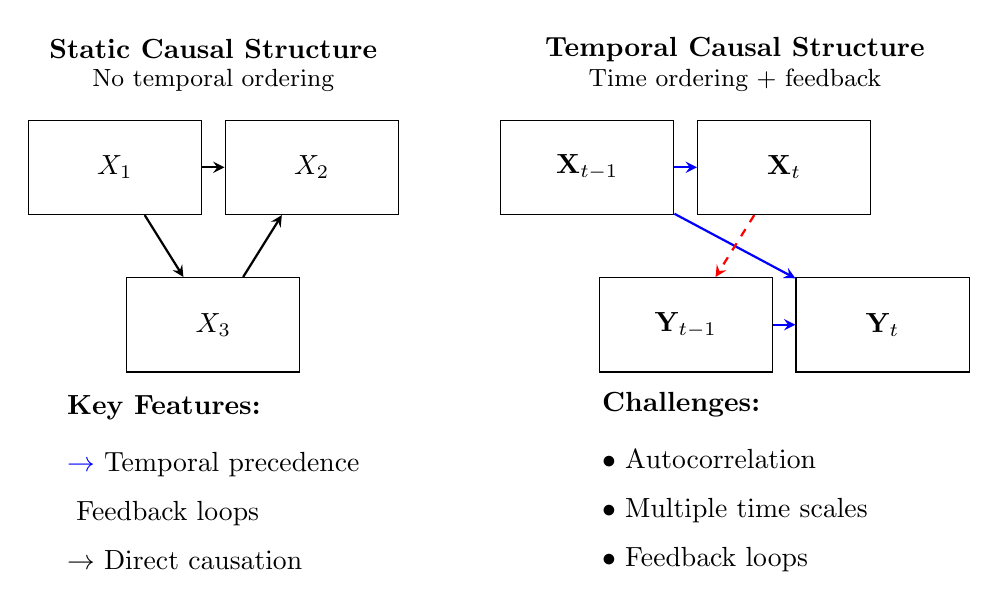
\begin{tikzpicture}[
			node distance=2.5cm,
			box/.style={rectangle, draw, minimum width=2.2cm, minimum height=1.2cm, align=center, font=\normalsize},
			arrow/.style={->, thick, >=stealth},
			time_arrow/.style={->, thick, blue, >=stealth},
			feedback/.style={->, thick, red, dashed, >=stealth}
		]
		% Static causal structure
		\node[box] (X1) at (0,0) {$X_1$};
		\node[box] (X2) at (2.5,0) {$X_2$};
		\node[box] (X3) at (1.25,-2) {$X_3$};

		\draw[arrow] (X1) -- (X2);
		\draw[arrow] (X1) -- (X3);
		\draw[arrow] (X3) -- (X2);

		\node at (1.25,1.5) {\textbf{Static Causal Structure}};
		\node at (1.25,1.1) {\small{No temporal ordering}};

		% Temporal causal structure
		\node[box] (T1) at (6,0) {$\mathbf{X}_{t-1}$};
		\node[box] (T2) at (8.5,0) {$\mathbf{X}_t$};
		\node[box] (T3) at (7.25,-2) {$\mathbf{Y}_{t-1}$};
		\node[box] (T4) at (9.75,-2) {$\mathbf{Y}_t$};

		\draw[time_arrow] (T1) -- (T2);
		\draw[time_arrow] (T3) -- (T4);
		\draw[time_arrow] (T1) -- (T4);
		\draw[feedback] (T2) -- (T3);

		\node at (7.875,1.5) {\textbf{Temporal Causal Structure}};
		\node at (7.875,1.1) {\small{Time ordering + feedback}};

		% Legend with better spacing
		\node[align=left, font=\normalsize] at (1.25,-4) {
			\textbf{Key Features:}\\[0.3cm]
			\textcolor{blue}{$\rightarrow$} Temporal precedence\\[0.2cm]
			\textcolor{red}{$\dashrightarrow$} Feedback loops\\[0.2cm]
			\textcolor{black}{$\rightarrow$} Direct causation
		};

		% Add explanatory text on the right
		\node[align=left, font=\normalsize] at (7.875,-4) {
			\textbf{Challenges:}\\[0.3cm]
			$\bullet$ Autocorrelation\\[0.2cm]
			$\bullet$ Multiple time scales\\[0.2cm]
			$\bullet$ Feedback loops
		};
	\end{tikzpicture}
	\caption[Temporal versus static causal structures]{Temporal versus static causal structures. Static structures (left) show contemporaneous relationships without temporal ordering, while temporal structures (right) incorporate time lags and can include feedback loops that violate acyclicity assumptions. The temporal setting provides natural directional constraints but introduces new challenges like autocorrelation and feedback mechanisms.}
	\label{fig:temporal_causal_structures}
\end{figure}

\subsubsection{Granger Causality: The Predictive Framework}

Granger causality, introduced by Nobel laureate Clive Granger in 1969, operationalizes causation through prediction: $\mathbf{X}$ causes $\mathbf{Y}$ if the past values of $\mathbf{X}$ help predict future values of $\mathbf{Y}$ beyond what $\mathbf{Y}$'s own past provides \cite{Granger}. This predictive notion, while not equivalent to true causation, provides a practical framework for identifying directed dependencies in time series. The method's intuitive appeal lies in its operational definition: if knowledge of $\mathbf{X}$'s history improves predictions of $\mathbf{Y}$'s future beyond what can be achieved using $\mathbf{Y}$'s own history alone, then $\mathbf{X}$ is said to Granger-cause $\mathbf{Y}$. This definition captures the essence of temporal precedence while remaining computationally tractable and statistically testable.

The theoretical foundation of Granger causality rests on the principle of temporal precedence and the assumption that causes contain information about their effects that is not available elsewhere. In the context of methane monitoring, this framework allows us to test whether, for example, temperature variations Granger-cause methane concentration changes, or whether vegetation indices provide predictive information about future methane emissions. The method's widespread adoption in econometrics, neuroscience, and climate science attests to its practical utility, despite its limitations in capturing true causal mechanisms.

\textbf{Mathematical Foundation}

Consider two time series $\{\mathbf{X}_t\}_{t \in \mathbb{Z}}$ and $\{\mathbf{Y}_t\}_{t \in \mathbb{Z}}$. The bivariate vector autoregressive (VAR) model of order $p$ captures their joint dynamics:

\begin{equation}
	\begin{bmatrix} \mathbf{Y}_t \\ \mathbf{X}_t \end{bmatrix} = \begin{bmatrix} \mathbf{c}_Y \\ \mathbf{c}_X \end{bmatrix} + \sum_{i=1}^{p} \begin{bmatrix} \mathbf{A}_{11}^{(i)} & \mathbf{A}_{12}^{(i)} \\ \mathbf{A}_{21}^{(i)} & \mathbf{A}_{22}^{(i)} \end{bmatrix} \begin{bmatrix} \mathbf{Y}_{t-i} \\ \mathbf{X}_{t-i} \end{bmatrix} + \begin{bmatrix} \boldsymbol{\varepsilon}_{Y,t} \\ \boldsymbol{\varepsilon}_{X,t} \end{bmatrix}
\end{equation}

where $\boldsymbol{\varepsilon}_t \sim \mathcal{N}(\mathbf{0}, \boldsymbol{\Sigma})$ represents innovation noise with covariance matrix $\boldsymbol{\Sigma}$.

$\mathbf{X}$ Granger-causes $\mathbf{Y}$ if the coefficients $\mathbf{A}_{12}^{(i)}$ are jointly non-zero. Formally, we test:
\begin{align}
	H_0 & : \mathbf{A}_{12}^{(1)} = \mathbf{A}_{12}^{(2)} = \cdots = \mathbf{A}_{12}^{(p)} = \mathbf{0} \\
	H_1 & : \exists i \in \{1, \ldots, p\} \text{ such that } \mathbf{A}_{12}^{(i)} \neq \mathbf{0}
\end{align}

This hypothesis is tested using an F-statistic comparing the restricted model (without $\mathbf{X}$) to the full model:
\begin{equation}
	F = \frac{(\text{RSS}_R - \text{RSS}_U)/p}{\text{RSS}_U/(T-2p-1)}
\end{equation}

where $\text{RSS}$ denotes residual sum of squares, subscripts $R$ and $U$ indicate restricted and unrestricted models, and $T$ is the time series length.

\textbf{The Granger Causality Index}

Beyond binary testing, the strength of Granger causality can be quantified as:

\begin{equation}
	\mathcal{F}_{\mathbf{X} \rightarrow \mathbf{Y}} = \ln\left(\frac{\sigma^2_{\boldsymbol{\varepsilon}_Y^R}}{\sigma^2_{\boldsymbol{\varepsilon}_Y^U}}\right)
\end{equation}

This index measures the logarithmic reduction in prediction error variance when including $\mathbf{X}$. For methane applications, it quantifies how much knowing temperature history improves emission prediction beyond autocorrelation alone.

\textbf{Limitations and Interpretations}

Granger causality differs from true causality in important ways:

\begin{enumerate}
	\item \textbf{Confounding}: Common drivers create spurious Granger causality. Seasonal cycles might make temperature Granger-cause vegetation indices without direct causal influence.

	\item \textbf{Mediation}: Indirect paths register as Granger causality. Temperature might Granger-cause methane through intermediate soil moisture effects.

	\item \textbf{Instantaneous effects}: Granger causality misses contemporaneous relationships occurring within the sampling interval.

	\item \textbf{Nonlinearity}: Linear VAR models miss nonlinear dependencies common in environmental systems.
\end{enumerate}

Despite limitations, Granger causality remains valuable for initial exploration of temporal dependencies, particularly when combined with domain knowledge to interpret results.

\textbf{Extensions to Address Limitations}

Modern extensions address various limitations:

\textbf{Nonlinear Granger Causality} using kernel methods \cite{Marinazzo2008}:
\begin{equation}
	\mathcal{F}_{\mathbf{X} \rightarrow \mathbf{Y}}^{\text{kernel}} = \frac{1}{2}\ln\left(\frac{\det(\mathbf{K}_{\mathbf{Y}\mathbf{Y}})}{\det(\mathbf{K}_{\mathbf{Y}\mathbf{Y}|\mathbf{X}})}\right)
\end{equation}

where $\mathbf{K}$ represents Gram matrices in reproducing kernel Hilbert space, capturing nonlinear dependencies.

\textbf{Spectral Granger Causality} decomposes causality by frequency:
\begin{equation}
	\mathcal{F}_{\mathbf{X} \rightarrow \mathbf{Y}}(\omega) = -\ln\left(1 - \frac{|\mathbf{H}_{\mathbf{Y}\mathbf{X}}(\omega)|^2 \sigma_{\mathbf{X}}^2}{\mathbf{S}_{\mathbf{Y}\mathbf{Y}}(\omega)}\right)
\end{equation}

This reveals whether causality operates at fast (daily weather) or slow (seasonal) time scales.

\textbf{Conditional Granger Causality} controls for confounders:
\begin{equation}
	\mathcal{F}_{\mathbf{X} \rightarrow \mathbf{Y}|\mathbf{Z}} = \ln\left(\frac{\sigma^2_{\boldsymbol{\varepsilon}_{\mathbf{Y}} | \mathbf{Z}}}{\sigma^2_{\boldsymbol{\varepsilon}_{\mathbf{Y}} | \mathbf{X},\mathbf{Z}}}\right)
\end{equation}

Essential when multiple drivers (temperature, precipitation, human activity) jointly influence methane.

\subsubsection{Information-Theoretic Approaches: Beyond Linear Prediction}

Information theory provides a model-free framework for detecting causal relationships in time series. Rather than assuming specific functional forms, these methods quantify directed information flow between variables, capturing both linear and nonlinear dependencies.

\textbf{Transfer Entropy: Directed Information Flow}

Transfer entropy (TE), introduced by Schreiber \cite{Schreiber2000}, quantifies the reduction in uncertainty about the next state of $\mathbf{Y}$ when the past of $\mathbf{X}$ is taken into account, beyond the information already contained in $\mathbf{Y}$'s own history. Unlike Granger causality, TE does not assume linearity or Gaussianity, making it particularly suitable for nonlinear and threshold-driven processes common in atmospheric and ecological systems.

Formally, for history vectors $\mathbf{X}^{(k)}_{t-\tau}=(X_{t-\tau},\ldots,X_{t-k\tau})$ and $\mathbf{Y}^{(l)}_{t-\tau}=(Y_{t-\tau},\ldots,Y_{t-l\tau})$, the lag-$\tau$ transfer entropy is:
\begin{equation}
	T_{\mathbf{X} \rightarrow \mathbf{Y}}^{(\tau)} = H(Y_t | \mathbf{Y}^{(l)}_{t-\tau}) - H(Y_t | \mathbf{Y}^{(l)}_{t-\tau},\mathbf{X}^{(k)}_{t-\tau}),
\end{equation}
where $H(\cdot)$ denotes Shannon entropy.

Equivalently, TE can be expressed as a conditional mutual information:
\begin{equation}
	T_{\mathbf{X} \rightarrow \mathbf{Y}}^{(\tau)} = I(Y_t; \mathbf{X}^{(k)}_{t-\tau} \mid \mathbf{Y}^{(l)}_{t-\tau}).
\end{equation}

A positive value $T_{\mathbf{X} \rightarrow \mathbf{Y}}^{(\tau)} > 0$ indicates that including $\mathbf{X}$'s past reduces the uncertainty of predicting $Y_t$, thus signaling a directional dependence. In methane monitoring, TE can capture, for example, how vegetation indices provide nonlinear predictive information about methane variability beyond seasonal autocorrelation.

\textbf{Estimation and Applications}

TE estimation in continuous, autocorrelated systems typically employs $k$-nearest-neighbour entropy estimators \cite{Kraskov2004} or kernel density methods. Statistical significance is assessed via surrogate time series, such as phase-randomised surrogates, which preserve autocorrelation but destroy directional coupling. These tests are critical in atmospheric contexts where strong seasonality can otherwise induce spurious TE.

Applications of TE in geosciences include quantifying nonlinear links between ENSO indices and rainfall \cite{tongal_forecasting_2021}, ecosystem-climate interactions \cite{Benocci2025}, and boreal-Arctic wetland methane emissions modulated by warming and vegetation activity \cite{Knox2024}. Its ability to detect episodic and nonlinear events, such as fire-driven methane release, makes TE a valuable complement to Granger causality.

\subsubsection{PCMCI: Scalable Causal Networks in Time Series}

While Granger causality and transfer entropy operate primarily in low-dimensional or pairwise settings, large-scale Earth observation datasets demand methods that handle many variables, strong autocorrelation, and hidden confounding. The PCMCI (Peter and Clark Momentary Conditional Independence) algorithm \cite{Runge2019} addresses these challenges by combining constraint-based causal discovery with temporal independence testing.

\textbf{Algorithmic Steps}

PCMCI proceeds in two stages, as illustrated in Figure~\ref{fig:pcmi_algorithm}:

\begin{enumerate}
	\item \textbf{Condition Selection (PC$_1$)}: For each candidate link $X_{t-\tau}^i \rightarrow Y_t^j$, the algorithm selects potential parents $\hat{P}(Y_t^j)$ by iteratively testing conditional independencies:
	      \begin{equation}
		      H_0: \mathbf{X}_{t-\tau}^i \perp \mathbf{Y}_t^j \; | \; \mathbf{S},
	      \end{equation}
	      where $\mathbf{S}$ is an increasing set of potential parents. Edges failing independence are removed. This phase reduces the search space by eliminating clearly spurious connections while preserving potentially causal relationships.
	\item \textbf{Momentary Conditional Independence (MCI)}: Surviving candidates are tested using an augmented conditioning set that includes both $\hat{P}(Y_t^j)$ and $\hat{P}(X_{t-\tau}^i)$ (excluding $X_{t-\tau}^i$ itself), reducing spurious detection from autocorrelation. This phase applies more stringent tests to the remaining candidate links, ensuring that only truly causal relationships survive.
\end{enumerate}

Significant links are oriented to respect temporal precedence, resulting in a lag-specific causal graph that captures the temporal structure of causal relationships in the system.

\begin{figure}[h!]
	\centering
	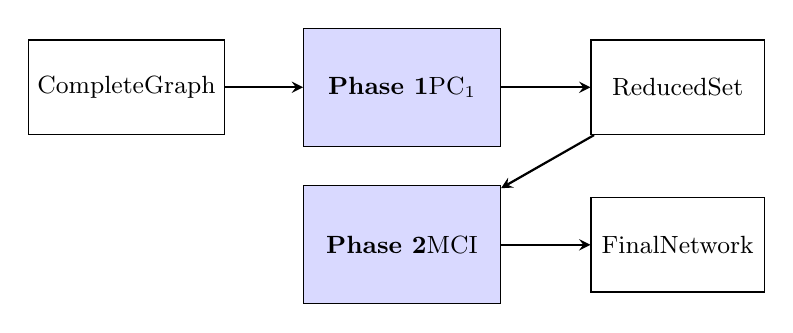
\begin{tikzpicture}[
			node distance=1.5cm,
			box/.style={rectangle, draw, minimum width=2.2cm, minimum height=1.2cm, align=center, font=\small},
			arrow/.style={->, thick, >=stealth},
			phase/.style={rectangle, draw, fill=blue!15, minimum width=2.5cm, minimum height=1.5cm, align=center, font=\small}
		]
		% Phase 1
		\node[phase] (phase1) at (0,0) {\textbf{Phase 1}\par PC$_1$};
		\node[box] (input1) at (-3.5,0) {Complete\par Graph};
		\node[box] (output1) at (3.5,0) {Reduced\par Set};

		\draw[arrow] (input1) -- (phase1);
		\draw[arrow] (phase1) -- (output1);

		% Phase 2
		\node[phase] (phase2) at (0,-2) {\textbf{Phase 2}\par MCI};
		\node[box] (output2) at (3.5,-2) {Final\par Network};

		\draw[arrow] (output1) -- (phase2);
		\draw[arrow] (phase2) -- (output2);

	\end{tikzpicture}
	\caption[The PCMCI algorithm workflow]{The PCMCI algorithm workflow. Phase 1 (PC$_1$) performs condition selection to reduce the search space, while Phase 2 (MCI) applies stringent conditional independence tests to identify the final causal network. This two-stage approach enables scalable causal discovery in high-dimensional, autocorrelated time series data.}
	\label{fig:pcmi_algorithm}
\end{figure}

\textbf{Strengths and Relevance}

PCMCI has three crucial advantages for methane applications. First, it scales efficiently to high-dimensional datasets such as MODIS land cover classes, meteorological drivers, and TROPOMI methane retrievals, making it suitable for comprehensive environmental monitoring systems. Second, it explicitly accounts for autocorrelation, which is particularly strong in atmospheric time series and can create spurious relationships if not properly handled. Third, it allows detection of both direct and indirect pathways, distinguishing, for instance, between temperature $\rightarrow$ soil moisture $\rightarrow$ methane and direct temperature $\rightarrow$ methane effects, providing more nuanced understanding of causal mechanisms.

Extensions such as PCMCI+ resolve contemporaneous effects, while LPCMCI incorporates latent confounding, producing Partial Ancestral Graphs (PAGs).

\textbf{Applications Related to Methane Monitoring}

Runge et al.~\cite{Runge2019_2} applied PCMCI to global climate networks, successfully disentangling drivers of ENSO dynamics. In methane studies, PCMCI has identified lagged wetland-to-\ch{CH_4} feedbacks with typical delays of 2–3 months \cite{Krich2020}, and guided causality-aware machine learning of boreal-Arctic wetland methane emissions \cite{Knox2024}. These results underscore PCMCI's suitability for satellite-based methane attribution.

\subsubsection{Synthesis of Temporal Causal Methods}

Each temporal method captures different aspects of causality: Granger causality excels in linear, stationary prediction; transfer entropy reveals nonlinear directional information; PCMCI scales to multivariate, autocorrelated systems. Table~\ref{tab:temporal_methods_comparison} provides a comprehensive comparison of these approaches, highlighting their key characteristics, assumptions, and suitability for methane monitoring applications. For robust inference in methane monitoring, we adopt a triangulation strategy combining these approaches, consistent with recent advances in causal machine learning \cite{Kaddour2022}. Agreement across methods increases confidence in inferred causal links, while divergence highlights sensitivity to assumptions or data limitations.

\begin{table}[h!]
	\centering
	\caption[Comparison of temporal causal discovery methods]{Comparison of temporal causal discovery methods for methane monitoring applications. Each method offers distinct advantages and limitations, making them complementary rather than competing approaches.}
	\label{tab:temporal_methods_comparison}
	\begin{tabular}{|>{\raggedright\arraybackslash}p{2.5cm}|>{\raggedright\arraybackslash}p{3.5cm}|>{\raggedright\arraybackslash}p{3.5cm}|>{\raggedright\arraybackslash}p{3.5cm}|}
		\hline
		\textbf{Method}   & \textbf{Key Assumptions}                                      & \textbf{Strengths}                                                                & \textbf{Limitations}                                                           \\
		\hline
		Granger Causality & Linear relationships, Stationarity, Gaussian innovations      & Computationally efficient, Well-established theory, Statistical testing           & Misses nonlinear effects, Sensitive to confounding, No contemporaneous effects \\
		\hline
		Transfer Entropy  & Model-free, No distributional assumptions                     & Captures nonlinear effects, No assumptions on functional form                     & Computationally intensive, Sensitive to parameter choices, Limited scalability \\
		\hline
		PCMCI             & Faithfulness, Temporal precedence, No contemporaneous effects & Handles high dimensions, Accounts for autocorrelation, Scalable to many variables & Requires sufficient data, Assumes no contemporaneous effects (basic version)   \\
		\hline
	\end{tabular}
\end{table}

The choice of temporal causal discovery method depends critically on the specific characteristics of the methane monitoring problem under investigation. For initial exploratory analysis of large-scale satellite datasets, Granger causality provides a computationally efficient first pass that can identify potential causal relationships for further investigation. When dealing with nonlinear processes such as wetland methane production under varying temperature and moisture conditions, transfer entropy offers the flexibility to capture complex, threshold-driven relationships that linear methods would miss. For comprehensive analysis involving multiple environmental drivers, atmospheric transport processes, and measurement characteristics, PCMCI's ability to handle high-dimensional, autocorrelated time series becomes essential.

The integration of these methods into a unified framework for methane causal discovery requires careful consideration of their complementary strengths. A hierarchical approach might begin with Granger causality to identify potential causal relationships in the data, followed by transfer entropy analysis to explore nonlinear aspects of these relationships, and finally PCMCI to construct a comprehensive causal network that accounts for the multivariate nature of the system. This triangulation strategy not only increases confidence in inferred causal relationships but also provides insights into the robustness of conclusions across different methodological assumptions.

Furthermore, the application of these methods to methane monitoring must account for the unique characteristics of satellite observations. Missing data due to cloud cover, varying spatial resolution, and the integration of emissions from multiple sources all pose challenges that require methodological adaptations. The development of robust preprocessing procedures, appropriate handling of missing data, and validation against ground-based measurements are essential components of a comprehensive temporal causal discovery framework for methane monitoring.

%%%%%%%%%%%%%%%%%%%%%%%%%%%%%%%%%%%%%%%%

\section{Problem Statement}
\label{sec:problem-statement}

\subsection{Scientific and Societal Context}

Methane (\ch{CH_4}) is a key climate forcer, with radiative effects and feedbacks that significantly amplify global warming. While it has a shorter atmospheric lifetime than carbon dioxide, its near-term radiative forcing is considerably stronger, and it exhibits complex temporal and spatial variability due to its diverse emission sources, including wetlands, agriculture, fossil fuels, and biomass burning. The accurate monitoring, attribution, and regulation of \ch{CH_4} emissions are essential for meeting national and international climate targets.

Recent advances in satellite-based remote sensing, particularly through missions such as TROPOMI (Sentinel-5P), GOSAT, and GHGSat, have enabled high-resolution observation of atmospheric methane over large spatial domains. However, most studies leveraging these data remain grounded in correlational or descriptive analyses. These methods are often blind to the underlying mechanisms and confounding factors that govern methane variability, reducing their explanatory power and utility for targeted mitigation.

The comprehensive literature review in Chapter \ref{chap:back} reveals fundamental gaps in current methodologies that prevent the development of causal frameworks for satellite-based methane monitoring. These gaps span from the lack of integrated multi-sensor analysis to the absence of ecosystem-specific approaches and comparative evaluation of causal versus correlational methods. This research directly addresses these critical limitations by developing a comprehensive temporal causal discovery framework specifically designed for satellite-based environmental monitoring.

\subsection{Policy Relevance and Validation Challenges}

The inability to establish causal relationships in methane monitoring has direct implications for climate policy and regulatory frameworks, including emission inventory verification, mitigation strategy evaluation, regulatory compliance, and international climate agreements like the Global Methane Pledge. These policy needs drive the requirement for robust validation strategies.

The proposed causal framework must address the validation challenges detailed in Chapter \ref{chap:back}, including cross-validation strategies, comparison with process-based models, sensitivity analysis, and uncertainty quantification to ensure robust and generalizable results for observational environmental data.

Collectively, these deficiencies constrain the derivation of robust mechanistic explanations for methane variability across ecosystems and time. Without causal integration of multi-source satellite data and domain-specific inference methods, attribution remains uncertain, limiting both scientific understanding and the development of spatially explicit mitigation strategies. Moreover, the lack of ecosystem-specific causal analysis prevents identification of biome-dependent mechanisms that could inform targeted intervention strategies. The absence of machine learning integration with causal inference further limits the development of interpretable and generalizable predictive models. Addressing these limitations is therefore essential to exploit the full diagnostic potential of Earth-observation records for climate-relevant gas monitoring and evidence-based policy.

\subsection{Scope and Expected Limitations}

This research focuses on developing and applying a comprehensive temporal causal discovery framework for satellite-based methane monitoring. The scope encompasses the integration of multi-sensor satellite observations (TROPOMI \ch{XCH_4}, MODIS land cover, ancillary atmospheric constituents) with advanced causal inference methods to identify mechanistic relationships governing methane variability across different ecosystems and temporal scales.

The research scope includes: (1) development of a unified framework integrating multiple causal discovery approaches; (2) ecosystem-stratified analysis across major land cover types; (3) systematic comparison of correlation-based and causal discovery methods; (4) exploration of machine learning and causal inference integration; (5) establishment of validation protocols for environmental causal inference; and (6) creation of open-source software tools for reproducible research.

By concentrating on globally retrieved methane concentrations, the study emphasizes causal relationships and mechanistic understanding between regions, seasons, and land cover types, rather than absolute emission flux estimates. This focus enables the development of transferable methodological approaches applicable to other environmental monitoring challenges while providing scientifically robust insights into methane system dynamics.

The following limitations are expected and acknowledged as inherent constraints of this research approach:

\begin{itemize}
	\item \textbf{Observational Constraints:} Satellite-derived methane concentrations are subject to measurement uncertainties and systematic biases arising from cloud contamination, surface reflectance effects, and retrieval algorithm differences. The spatial resolution ($\sim$7~km) is insufficient to detect small-scale emission sources, necessitating focus on regional patterns rather than point-source attribution. These limitations are inherent to current satellite technology and retrieval methodologies.

	\item \textbf{Temporal Scope Limitations:} The analysis is limited to the TROPOMI era (2017-present), which constrains the assessment of long-term trends and decadal-scale climate feedbacks. This limitation is imposed by the availability of satellite data and represents a fundamental constraint on the temporal depth of the analysis.

	\item \textbf{Causal Inference Limitations:} Since controlled experiments on the atmosphere are not feasible, the analysis relies on statistical causality tests under specific assumptions, such as the absence of unmeasured confounders. These limitations are inherent to observational environmental studies and require careful methodological consideration.

	\item \textbf{Computational Constraints:} The application of causal methods to large satellite datasets requires careful consideration of computational efficiency and scalability. These limitations are expected given the volume and complexity of satellite data and the computational demands of causal inference algorithms.

	\item \textbf{Software Development and Maintenance:} The creation of comprehensive open-source software tools requires ongoing maintenance, documentation, and user support that extends beyond the research timeline. While the initial framework development is within scope, long-term software sustainability depends on community adoption and institutional support.
\end{itemize}

%%%%%

\section{Research Objectives}
\label{sec:research-objectives}

\subsection{Main Objective}

To discover and map potential causal relationships between atmospheric methane concentrations and environmental drivers using causal discovery methods applied to satellite-based time series data, comparing correlation-based and causal inference approaches, and exploring the integration of machine learning with causal inference for methane analysis, with the goal of identifying which variables may causally influence methane variability across different land cover types and regions.

\subsection{Specific Objectives}

\begin{enumerate}
	\item \textbf{Develop Temporal Causal Discovery Framework:} Design and implement a unified framework for discovering causal relationships in satellite-based methane time series, integrating multi-sensor data (TROPOMI \ch{XCH_4}, MODIS land cover, co-constituents) with temporal causal discovery methods (Granger causality, transfer entropy, PCMCI+).

	\item \textbf{Characterize Ecosystem-Specific Causal Patterns:} Identify and quantify causal relationships between methane concentrations and environmental drivers across different land cover types, revealing biome-specific mechanisms of methane variability.

	\item \textbf{Compare Correlation and Causal Discovery Approaches:} Systematically compare correlation-based analysis with causal discovery methods to evaluate their respective strengths, limitations, and complementarity in identifying methane-environmental relationships, providing insights into when each approach is most appropriate.

	\item \textbf{Study Machine Learning and Causal Inference Approaches:} Study existing machine learning and causal inference methods for methane analysis, exploring how predictive models can enhance causal discovery and how causal knowledge can improve machine learning interpretability and generalization.

	\item \textbf{Validate Causal Discovery in Environmental Systems:} Establish robust validation protocols for causal inference in observational environmental data, addressing challenges of autocorrelation, confounding, and measurement uncertainty in satellite time series.

	\item \textbf{Create Open-Source Software Ecosystem:} Develop and disseminate a comprehensive software package implementing the complete causal discovery pipeline, enabling reproducible research and broader adoption in environmental monitoring.
\end{enumerate}

These objectives reflect the current scope and direction of an ongoing research project and may be refined as new findings, challenges, or opportunities emerge during its development.

%%%%%

\section{Proposed Solution and Innovation}
\label{subsec:proposed-solution}

This research proposes a scalable, statistically grounded framework for causal discovery in environmental satellite time series, centered on methane. The framework addresses the identified gaps through unified spatiotemporal data assembly (TROPOMI \ch{XCH_4} + MODIS land cover + ancillary data), causal inference via time-lagged statistical tests (Granger causality, transfer entropy, PCMCI), stratified analysis by land cover type, and attribution logic through directed acyclic graphs (DAGs) for policy-relevant interpretation.

This proposal differs from previous studies by not only detecting "where" methane is elevated but also exploring "why" it occurs through validated causal paths where possible, thus attempting to transition from descriptive geospatial analysis toward mechanistic environmental understanding.

\subsection{Scientific and Policy Relevance}
\label{subsec:scientific-relevance}

The proposed causal framework addresses a key methodological gap in satellite-based methane monitoring by exploring spatiotemporally explicit attribution, delivering open-source reproducible tools, supporting regulatory and policy efforts where feasible, and aligning with ESA, Global Methane Pledge, and IPCC priorities. The framework also provides a transferable methodology applicable to other environmental variables and domains, potentially strengthening the scientific foundation for region-specific mitigation planning and improving transparency in emissions accounting.

\subsection{Expected Results}

\begin{itemize}
	\item Causal graphs showing discovered relationships between methane and environmental variables across different land cover types.
	\item Identification of which environmental variables (e.g., temperature, precipitation, vegetation indices) show potential causal relationships with methane concentrations.
	\item Maps of discovered causal patterns aggregated by region and season, subject to data quality and methodological constraints.
	\item Comparison of results from different causal discovery methods (Granger causality, transfer entropy, PCMCI) to assess consistency and robustness.
\end{itemize}

\subsection{Scientific Contributions}

\begin{itemize}
	\item A reproducible causal discovery framework for environmental satellite time series.
	\item Methodological innovation in combining land cover stratification with temporal causal discovery methods.
	\item Discovery of ecosystem-specific patterns in methane-environmental variable relationships across diverse biomes.
	\item Enhanced understanding of satellite methane retrievals through causal network analysis.
	\item Open-access documentation, scripts, and visual tools for the scientific community.
\end{itemize}

%%%%%

\section{Scope and Limitations}

This research focuses on leveraging satellite-based observations and causal analysis to improve the monitoring of methane emissions. The scope emphasizes relative differences and causal relationships between regions, seasons, and land cover types, rather than absolute emission flux estimates. Specific technical limitations of satellite observations are detailed in the preceding section, while methodological constraints are addressed in Chapter~\ref{chap:methodology}.

Key scope boundaries include: (i) focus on atmospheric methane concentrations rather than direct emission quantification, (ii) emphasis on regional patterns rather than point-source attribution, and (iii) restriction to observational causal relationships detectable from satellite data, excluding broader socio-economic drivers. The methodological limitations of causal inference approaches and computational constraints are comprehensively addressed in Chapters~\ref{chap:methodology} and \ref{chap:evaluation}, respectively.
%%%%%

\section{Organization of the Document}
This document is organized into six main chapters.

\textbf{Chapter 1 (Introduction)} provides background on the problem of monitoring methane emissions, the role of causal analysis, the problem statement and research gaps, the relevance of the research, and the objectives of the study. It also outlines the scope of our work and its limitations, as well as the expected outcomes.

\textbf{Chapter 2 (Literature Review)} reviews the state of the art in relevant domains: satellite-based methane monitoring techniques, \gls{causal_inference} methods in environmental science, interactions between land cover and atmospheric composition, and existing approaches to causal analysis in time series data. Identifies findings from previous studies and highlights open challenges that motivate our research.

\textbf{Chapter 3 (Methodology)}details the methodology for this PhD project's causal analysis. It integrates established principles of causal inference, remote sensing, and computational modeling, describing the staged workflow encompassing data handling, framework validation, and large-scale satellite time series analysis. The methodology is designed to uncover robust and interpretable spatiotemporal causal relationships governing methane variability, emphasizing scalability, reproducibility, and alignment with Earth observation standards.

\textbf{Chapter 4 (Preliminary Results)} presents initial results obtained from applying parts of our framework to sample datasets and simple case studies. These early findings serve to demonstrate the feasibility of the approach and inform any necessary refinements to the methodology.

\textbf{Chapter 5 (Research Plan)} delineates the plan for the remaining research, including a timeline of activities and milestones, potential risks with mitigation strategies, and a dissemination plan for sharing results with the scientific community and stakeholders.

\textbf{Chapter 6 (Conclusion)} summarizes the contributions of the work, reflects on the findings, and discusses the limitations of the study and future work, tying the research back to the broader context and objectives outlined in the introduction.

